\documentclass[a4paper,9pt]{article}
%\documentclass[a4paper,9pt]{book}
%\documentclass[11]{amsbook}
%\documentclass[a4paper,11pt]{book}
\usepackage{ucs}
\usepackage[utf8x]{inputenc}
\usepackage[T1]{fontenc}
\usepackage{amsmath,amsfonts,amssymb,amsthm}
\usepackage{pb-diagram,graphicx}
\usepackage{graphicx}
\usepackage{epsfig}
\usepackage{graphics}
%\usepackage[pst-3d]{pstricks}
%\usepackage{psfrag}
\usepackage{latexsym}
\usepackage{multicol}
\usepackage{times}
%\usepackage{bbold}
%\usepackage{bbold}
%\usepackage{dsfont}
%\usepackage{german}
%\usepackage{german}
%\usepackage[ansinew]{inputenc}
%\usepackage[utf8]{inputenc}
\usepackage[ngerman]{babel}
%\usepackage[english,ngerman]{babel}
\usepackage{listings}
\usepackage{color}
%\usepackage{subfig}
\usepackage{subfigure}
%
\usepackage[table]{xcolor}  
%
%\usepackage{movie15}
%\usepackage{hyperref}
%\usepackage{movie15}
\usepackage{bibgerm}
%
\usepackage{multirow}
%\markboth
%
%
\usepackage{lscape} % querformat
 \usepackage{fancyhdr}
%
%
% \pagestyle{fancy}
% \fancyhf{}
% %\fancyheadoffset[RO,LE]{30pt}
% \fancyhf{}
% \fancyhead[OR,EL]{\thepage}
%%\fancyhead[EL]{\thepage}
%%
% \fancyhead[LO]{\rightmark}
% \fancyhead[ER]{\leftmark}
% %\fancyfoot[C]{\thepage}
%%
 \renewcommand
 \headrule{{\color{black}%
 \hrule height 0.5pt width \headwidth
 %\vspace{1pt}%
 %\hrule height 1pt
 %width\headwidth
 %\vspace{-4pt}
 }}
%
\newtheorem{theorem}{Theorem}[subsection]
\newtheorem{definition}[theorem]{Definition}
\newtheorem{lemma}[theorem]{Lemma}
\newtheorem{corollary}[theorem]{Corollary}
\newtheorem{proposition}{Proposition}
\newtheorem{remark}{Remark}
\newtheorem{example}[theorem]{Example}
\newtheorem{assumption}{Assumption}
\newtheorem{conjecture}{Conjecture}
\newcommand{\TT }{ \mathcal{T}}
%
\newcommand{\e }{ \varepsilon}
\newcommand{\om }{ \omega}
\newcommand{\Om }{ \Omega}
\newcommand{\de }{ \delta}
\newcommand{\dn }{ \partial_n}
\newcommand{\dna }{ \partial_{n_1}}
\newcommand{\dnb }{ \partial_{n_2}}
\newcommand{\dnx }{ \partial_{n_x}}
\newcommand{\dnxi }{ \partial_{n_\xi}}
\newcommand{\curl }{ \nabla \times}
\newcommand{\ue }{u_{\e,\gamma}}
\newcommand{\pe }{p_{\e,\gamma}}
\newcommand{\s}{\sum_{j=1}^2}
\newcommand{\Dj }{ \partial_j}
\newcommand{\gj}{\mathcal{G}_j}
\newcommand{\bg}{\bar{g}}
\newcommand{\hL}{\hat{L}}
\newcommand{\hQ}{\hat{Q}}
\newcommand{\hM}{\hat{M}}
\newcommand{\hu}{\hat{u}}
\newcommand{\hx}{\hat{x}}
\newcommand{\hq}{\hat{q}}
\newcommand{\tu}{\tilde{u}}
\newcommand{\tq}{\tilde{q}}
\newcommand{\tphi}{\tilde{\phi}}
\newcommand{\bu}{\bar{u}}
\newcommand{\ou}{\overline{u}}
\newcommand{\uu}{\underline{u}}
\newcommand{\tw}{\tilde{w}}
\newcommand{\hw}{\hat{w}}
\newcommand{\hS}{\hat{S}}
\newcommand{\hbF}{\hat{\boldsymbol{F}}}
\newcommand{\tG}{\tilde{G}_\delta}
\newcommand{\ti}{\tilde{I}_\delta}
\newcommand{\tyd}{\tilde{y}_\delta}
\newcommand{\A }{ \mathcal{A}}
\newcommand{\HH }{ \mathcal{H}}
\newcommand{\B }{ \mathcal{B}}
\newcommand{\C }{ \mathcal{C}}
\newcommand{\I }{ \mathcal{I}}
\newcommand{\Ie }{ \mathcal{I}_{\e,\gamma}}
\newcommand{\Ae }{ \mathcal{A}_{\e,\gamma}}
\newcommand{\Be }{ \mathcal{B}_{\e,\gamma}}
\newcommand{\T }{ \mathcal{T}}
\newcommand{\OO }{ \mathcal{O}}
\newcommand{\KK }{ \mathcal{K}}
\newcommand{\N }{ \mathcal{N}}
\newcommand{\R }{ \mathcal{R}}
\newcommand{\RR }{ \mathbb{R}}
\newcommand{\Sh }{ \mathcal{S}}
\newcommand{\xx}{\emph{\textbf{x}}}
\newcommand{\xxx}{\textbf{x}}
\newcommand{\nn}{\textbf{n}}
\newcommand{\buu}{\boldsymbol{u}}
\newcommand{\bFF}{\boldsymbol{F}}
\newcommand{\bQQ}{\boldsymbol{Q}}
\newcommand{\baa}{\boldsymbol{a}}
\newcommand{\bxx}{\boldsymbol{x}}
\newcommand{\brr}{\boldsymbol{r}}
\newcommand{\byy}{\boldsymbol{y}}
\newcommand{\bbb}{\boldsymbol{b}}
\newcommand{\bww}{\boldsymbol{w}}
\newcommand{\bgg}{\boldsymbol{g}}
\newcommand{\bbuu}{\bar{\boldsymbol{u}}}
\newcommand{\bnn}{\boldsymbol{n}}
\newcommand{\bcc}{\boldsymbol{n}}
\newcommand{\bdd}{\boldsymbol{d}}
\newcommand{\bzz}{\boldsymbol{0}}
\newcommand{\oa}{\Om_1^\e}
\newcommand{\ob}{\Om_2^\e}
\newcommand{\ua}{u_1^\e}
\newcommand{\ub}{u_2^\e}
\newcommand{\ra}{\mathcal{R}_{2,\e}^1}
\newcommand{\raa}{\mathcal{R}_{1,\e}^1}
\newcommand{\sa}{\mathcal{S}_{2,\e}^1}
\newcommand{\saa}{\mathcal{S}_{1,\e}^1}
\newcommand{\rb}{\mathcal{R}_{2,\e}^2}
\newcommand{\Sb}{\mathcal{S}_{2,\e}^2}
\newcommand{\LL }{ \mathcal{L}}
\newcommand{\DD }{ \mathcal{D}}
\newcommand{\JJ }{ \mathcal{J}}
\newcommand{\SSg }{ \mathcal{SG}}
\newcommand{\PP }{ \mathcal{P}}
\newcommand{\hJJ }{ \hat{\mathcal{J}}}
\newcommand{\hJ }{ \hat{J}}
%
\newcommand{\uup }{ \buu' }
\newcommand{\ppp }{ \bpp' }
\newcommand{\pp }{ p' }
\newcommand{\phip }{ \phi' }
\newcommand{\zp }{ \bz' }
%
\newcommand{\bvv}{\boldsymbol{v}}
\newcommand{\bUU}{\boldsymbol{U}}
\newcommand{\btau}{\boldsymbol{\tau}}

%
\newcommand{\bpp}{\boldsymbol{p}}
\newcommand{\bz}{\boldsymbol{z}}
\newcommand{\bx}{\boldsymbol{x}}

\newcommand{\bvt}{\tilde{\bvv}}
\newcommand{\but}{\tilde{\buu}}
\newcommand{\bxt}{\tilde{\bxx}}
\newcommand{\bxb}{\bar{\bxx}}
%
\newcommand{\yu}{\byy^{\buu}}
%
\numberwithin{equation}{section}
%
\numberwithin{figure}{section}
%
\renewcommand{\qedsymbol}{$\blacksquare$}
\definecolor{light-gray}{gray}{0.7}
\definecolor{dark-gray}{gray}{0.4}
\definecolor{orange}{rgb}{1,0.5,0}
%
\definecolor{dgreen}{rgb}{0.,0.6,0.}
\definecolor{dred}{rgb}{0.6,0.,0.}
\definecolor{dorange}{rgb}{0.9,0.5,0.}
\definecolor{dblue}{rgb}{0.,0.,0.6}
\definecolor{grey}{rgb}{0.5,0.5,0.5}


%\numberwithin{lemma}{section}
%
%\numberwithin{theorem}{section}
%
%\numberwithin{definition}{section}
%
%\pagenumbering{roman}
%\thispagestyle{empty}
%\title{BMW-Projekt}
%\author{Martin Kanitsar}
%
%
%
\begin{document}
\begin{figure}
 \begin{center}
   
\includegraphics[width=12.5cm,height=1.87cm]{head.jpg}
 \end{center}
\end{figure}
%
\hrulefill
%
%\tableofcontents
\vspace{5mm}
\begin{center}\bf{\huge{Handbuch zur Software}}\end{center}
\vspace{10mm}
\begin{center}\large{``Form- und Topologieoptimierung''}\end{center}
\vspace{10mm}
%\begin{center}\large{``Teil I: Formoptimierung bei Strömungen ohne Filtermodell.''}\end{center}
%\begin{center}\large{``Teil II: Verwendung eines Filtermodells.''}\end{center}

\vspace{10mm}
\begin{itemize}
\item Prof. Dr. M. Hintermüller (Humboldt-Universität zu Berlin)
\vspace{5mm}
\item Dr. K. Knall (Mathtec, Wien)
\vspace{5mm}
\item MMag. M. Kanitsar (Mathtec, Wien/Universität Graz)
\end{itemize}
\vspace{10mm}
%\begin{center}Besprechung: 2012, BMW-Steyr\end{center}
\vspace{10mm}
Software-Version: 1612.\\
$ $\\
\vspace{10mm}
\hrulefill
%
\begin{figure}[b]
\begin{center}
\subfigure{
   
\includegraphics[width=3.5cm,height=1.38cm]{HU.jpg}}
\subfigure{
    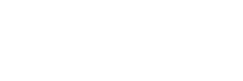
\includegraphics[width=3.5cm,height=1.38cm]{empty.jpg}}
\subfigure{
    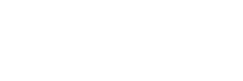
\includegraphics[width=2.5cm,height=1.38cm]{empty.jpg}}
\subfigure{
   
\includegraphics[width=1.69cm,height=1.19cm]{ifb.jpg}}
   \end{center}
\end{figure}
\newpage
%
%\maketitle
\tableofcontents
\newpage
%
%\part{Formoptimierung bei Strömungen ohne Filtermodell}
%
\section{Installation}
\subsection{Ordnerstrukturierung und Kompilieren der Applikationen}
Zur Verwendung der Form- und Topologieoptimierung ist die Standard-Installation von OpenFOAM (\$FOAM\_APP/solvers/incompressible/) um folgende Applikationen zu erweitern:\\
\begin{tabular}{ll}
 \parbox{5cm}{
 \begin{itemize}
%
\item generateFieldsFoam
\item shapeGradientWall,
\item shapeGradientCCM,
\item setupShapeGradientCCM,
\item shapeGradientAddSTL,
 \end{itemize}}
 &
 \parbox{5cm}{
 \begin{itemize}
\item shapeGradientCloseAll,
\item topoOpt,
\item topoOptCloseAll,
\item topoExtractSTL.\\
$ $\\
 \end{itemize}}
\end{tabular}\\
Der Ordner InitialSGccm ist in das Verzeichnis  \$FOAM\_RUN/tutorials/ zu kopieren. Die Konsolen-Befehle zur Installation befinden sich im shell-script \emph{installShapeGradient.sh}.\\
%
\section{Geometriedaten}
\subsection{Speicherstruktur der Daten im STL-Format}
Die Geometriedaten sind im Ordner \emph{initial\_stl} anzulegen. 
Neben der Bauraumgeometrie (\textbf{bds.stl}) werden die Oberflächen in 4 Dateien im STL-Format gespeichert (\textbf{inlet.stl}, \textbf{fixed.stl}, \textbf{wall.stl}, \textbf{outlet.stl}).\\
Zur Veranschaulichung dient die Testgeometrie \emph{M23} mit 2 Inlets, 3 Outlets und einer zusätzlichen fixen Geometrie (siehe Tabelle \ref{tab:stlDaten1}).
%\hspace{-60pt}
%\vrule{}
\begin{figure}[htbp]
  \centering
    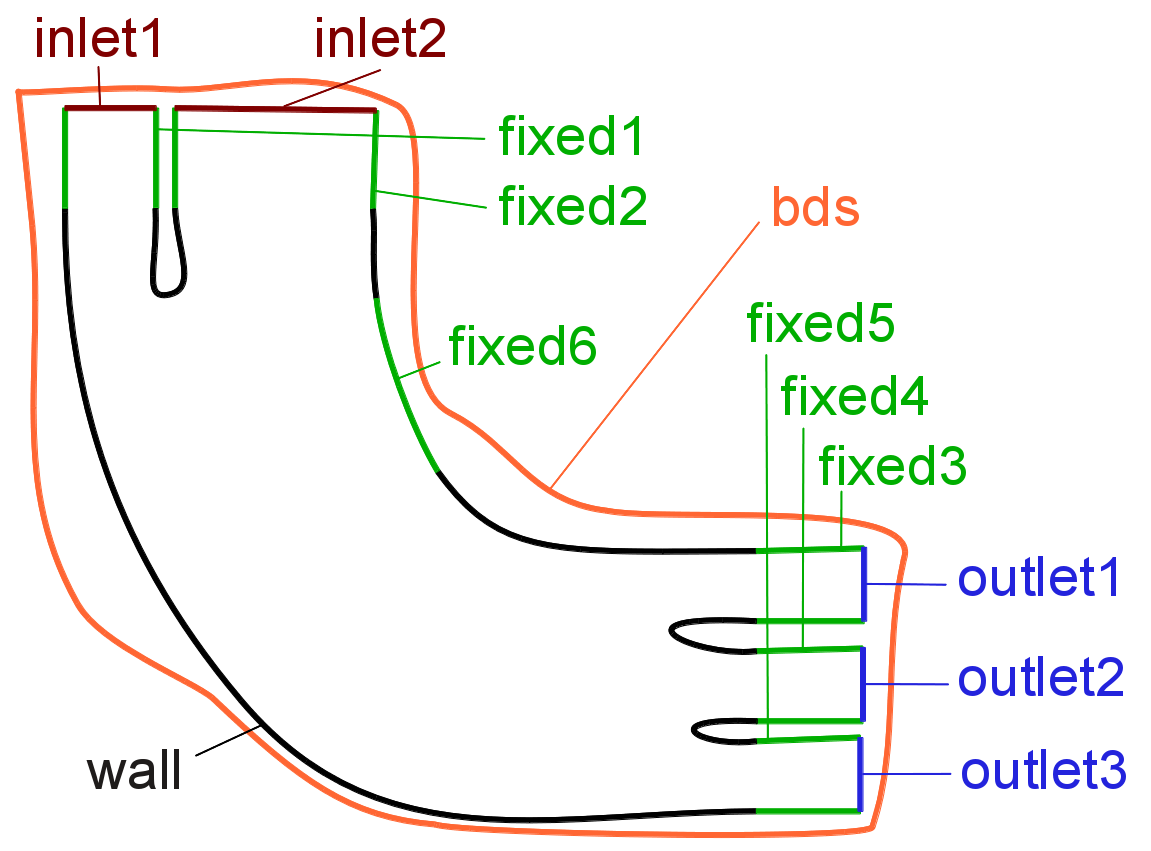
\includegraphics[scale=0.45]{skizze_designSpace4.png}
    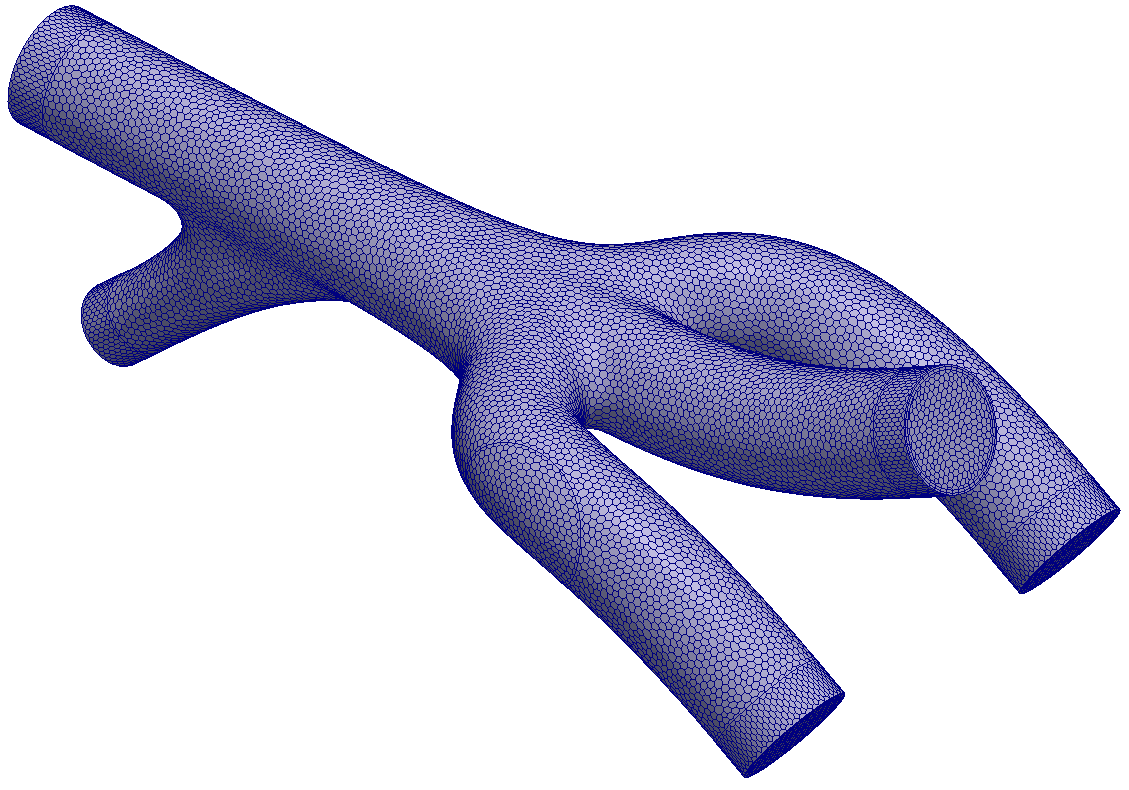
\includegraphics[scale=0.15]{M23all.png}   
  \caption{Links: Skizze Geometriedaten, rechts Testgeometrie M23.} 
\label{fig:skizzeBauraum}
\end{figure}
%
%
\begin{table}[h]
\centering
\begin{tabular}{|p{0.9cm}|p{4.6cm}|p{3.7cm}|p{1.2cm}|} %lcrp
\hline
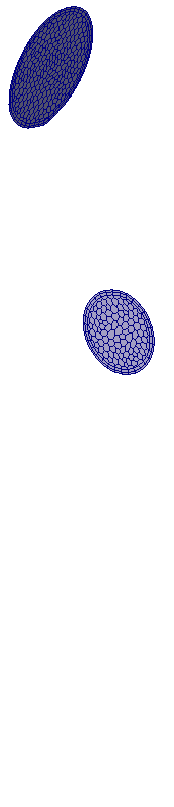
\includegraphics[scale=0.35]{M23in.png}  &  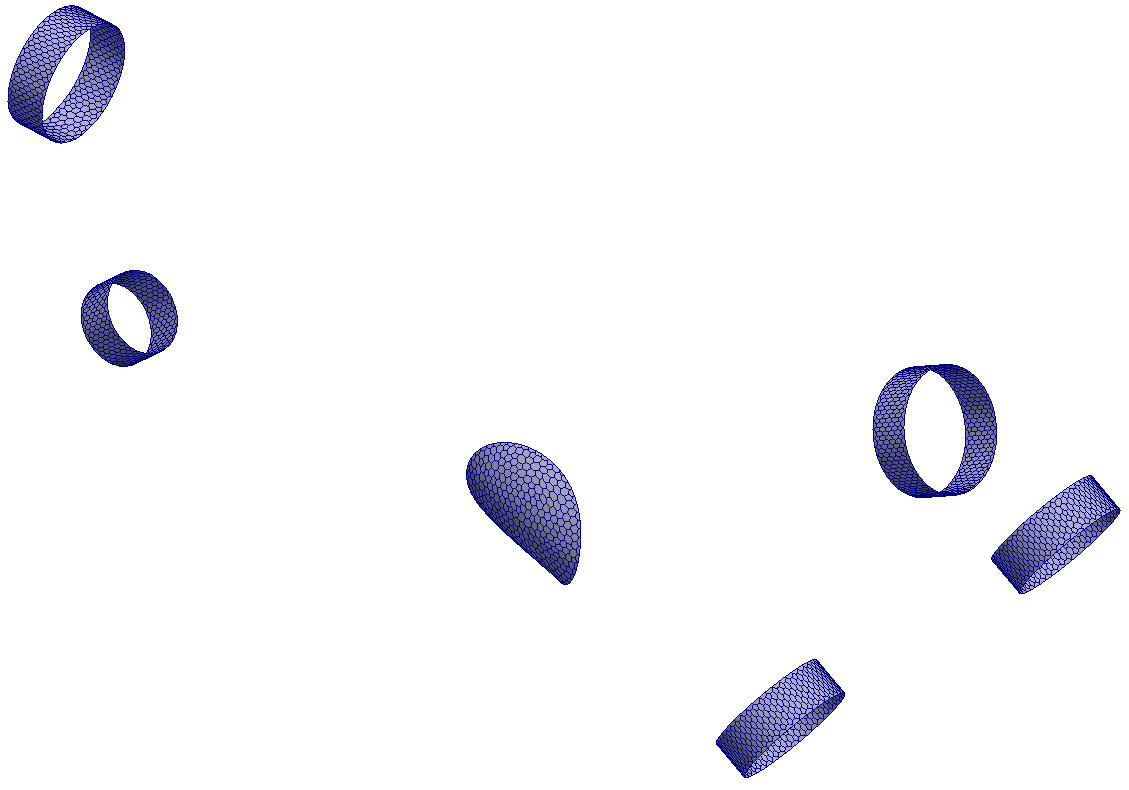
\includegraphics[scale=0.1]{M23fixed.png}   &   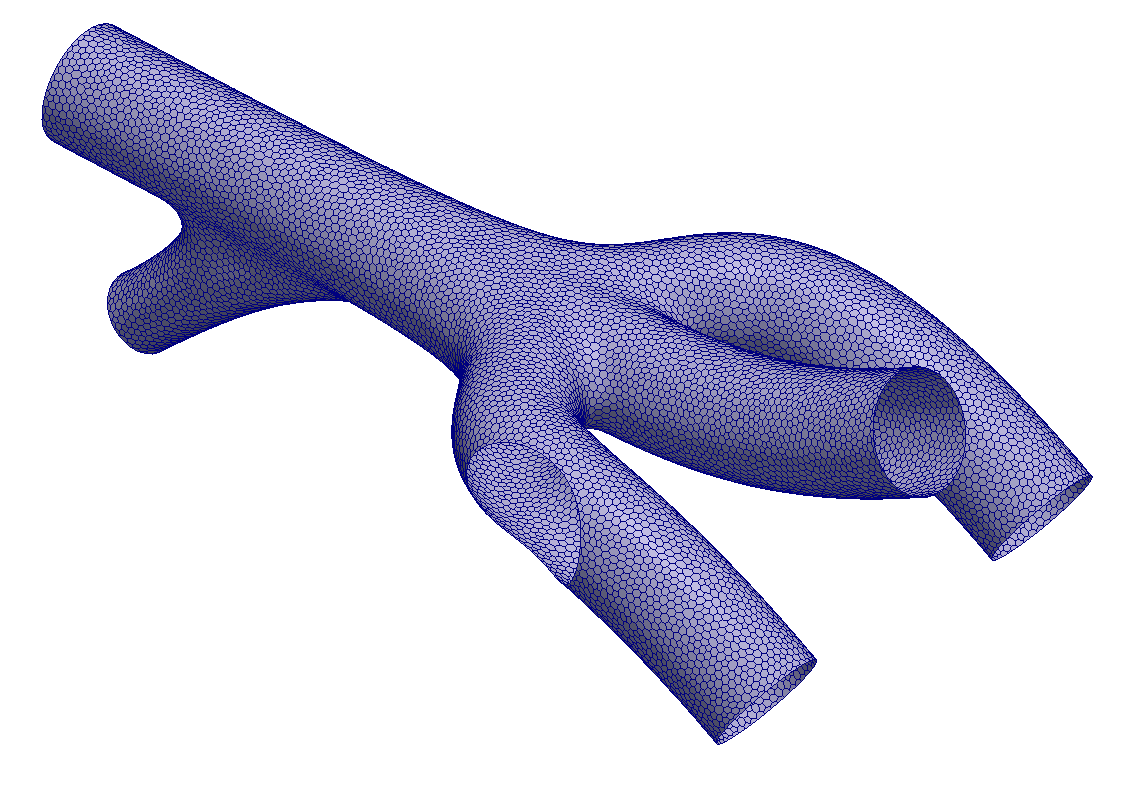
\includegraphics[scale=0.1]{M23wall.png}  &   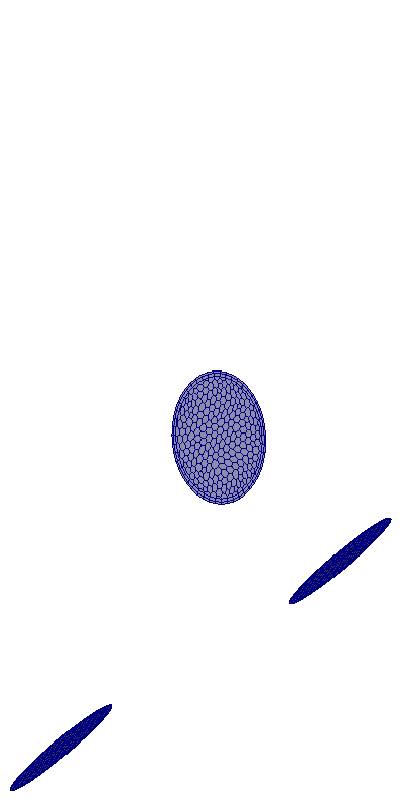
\includegraphics[scale=0.35]{M23out.png}  \\
\hline
\textcolor{dred}{inlet.stl}  &  \textcolor{dgreen}{fixed.stl}      &   wall.stl &  \textcolor{dblue}{outlet.stl} \\
\hline
\textcolor{dred}{inlet1} \quad \textcolor{dred}{inlet2}  &  
\textcolor{dgreen}{fixed1} \textcolor{gray}{[inlet1]} ,  \textcolor{dgreen}{fixed2} \textcolor{gray}{[inlet2] \;} 
\textcolor{dgreen}{fixed3} \textcolor{gray}{[outlet1]} ,  \textcolor{dgreen}{fixed4} \textcolor{gray}{[outlet2]}
\textcolor{dgreen}{fixed5} \textcolor{gray}{[outlet3]} ,  \textcolor{dgreen}{fixed6}
    &   wall.stl &  \textcolor{dblue}{outlet.stl} \\
\hline
\end{tabular}
\caption{Geometriedaten im STL-Format.}\label{tab:stlDaten1}
\end{table}
%
\begin{table}[h]
\centering
\begin{tabular}{|p{1.3cm}|p{5.1cm}|p{4cm}|} %lcrp
\hline
\cellcolor{light-gray} Dateiname & \cellcolor{light-gray} Bezeichnung & \cellcolor{light-gray} Beschreibung\\
\hline
inlet.stl  &  inlet1, inlet2, inlet3          &   Einströmgeometrien.\\
\hline
outlet.stl  &  outlet1, outlet2, outlet3            &   Ausströmgeometrien.\\
\hline
fixed.stl  &  fixed1, fixed2, fixed3, fixed4, fixed5, fixed6, fixed7, fixed8, fixed9 & Geometriedaten der fixen Bereiche.\\
\hline
wall.stl  &  wall        & Geometriedaten des zu formoptimierenden Bereiches.\\
\hline
bds.stl &  bds & Geometriedaten des Bauraumes.\\
\hline
\end{tabular}
\caption{Geometriedaten im STL-Format.}\label{tab:stlDaten2}
\end{table}
$ $\\
Jeder Ein- und Ausströmbereich besitzt jeweils eine fixe Geometrie, die die Verbindung zu der zu formoptimierenden Geometrie beschreibt.
Zusätzlich kann der Benutzer fixe Geometrien festlegen die lediglich mit der zu formoptimierenden Geometrie verbunden sind (z.B.: fixed6 in Testgeometrie M23). \\
Die \textbf{Nummerierung der fixen Geometrien} erfolgt fortlaufend, beginnend bei den Verbindungen zur Einströmgeometrie, 
weiterführend bei den Verbindungen zur Ausströmgeometrie und am Ende bei den fixen Geometrien, die nur mit der zu formoptimierenden Geometrie verbunden sind.  
%
$ $\\
Bei der Wahl der Bauraumgeometrie sollte darauf geachtet werden, 
dass die Startgeometrie vollständig im zulässigen Bereich liegt 
und über die Interfaces inti\_free-geom\_fixed-inlet und into\_free-geom\_fixed-outlet 
hinausreicht (siehe Abbildung \ref{fig:skizzeBauraum}). 
%
%
\subsection{Modellierung der Ein-/Ausströmbereiche}
Folgende Aufbereitung dient dazu, die Modellierung einer Anwendung hinsichtlich der Oberflächengeometrien der Einströmbereiche und der Ausströmbereiche
 darzustellen.\\
%Möglicherweise wurde die Modellierung einer Anwendung hinsichtlich der Oberflächengeometrien des Einströmbereiches und des Ausströmbereiches
% nicht klar genug dargestellt.\\
\subsubsection{Einströmbereiche}
Es können beliebig viele Einströmbereiche festgelegt werden. 
Ein Einströmbereich kann auch aus mehreren nicht zusammenhängenden Geometrien bestehen. 
Auszeichnend für einen Einströmbereich ist nicht die Form/Topologie sondern sind die physikalischen Eigenschaften, wie z.B.: Einströmgeschwindigkeit.
\begin{itemize}
 \item Daher kann eine Anwendung mit gleicher Einströmgeschwindigkeit auch mit einem Einströmbereich modelliert werden (linke Grafik in Abb. \ref{fig:multInlet}).
\item Gibt es in der Anwendung unterschiedlichen Einströmgeschwindigkeiten so sind unterschiedliche Einströmbereiche festzulegen (rechte Grafik in Abb. \ref{fig:multInlet}). 
\end{itemize}
\begin{figure}[htbp]
\centering
 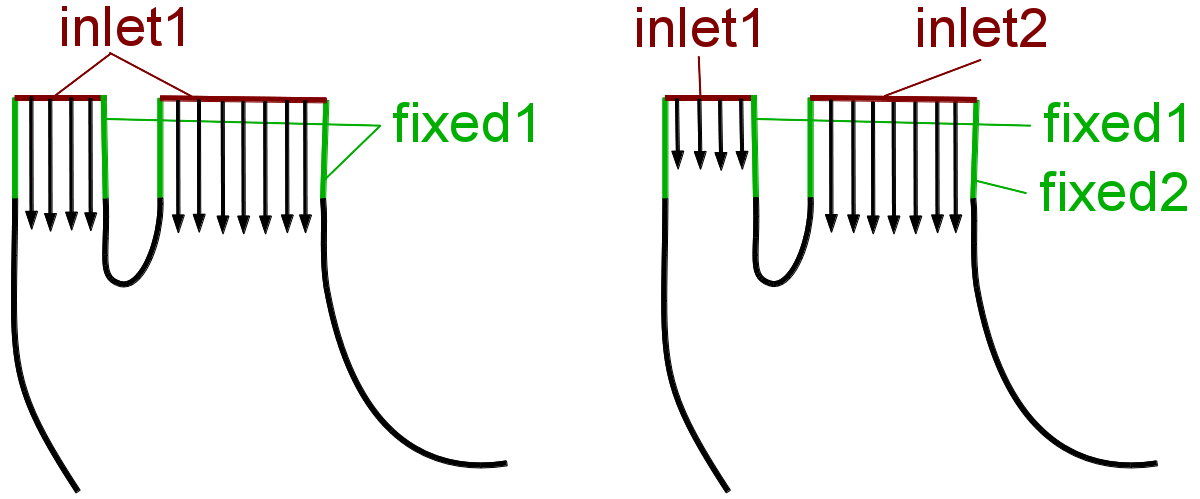
\includegraphics[scale=0.53]{inletMULT.png}   
\caption{Einströmbereiche.}
\label{fig:multInlet}
\end{figure}
\newpage
\subsubsection{Ausströmbereiche}
Es können beliebig viele Ausströmbereiche festgelegt werden.
Analog zur Festlegung der Einströmbereiche ist die Festlegung der Ausströmbereiche anhand der physikalischen Eigenschaften zu treffen. 
Bei den bisherigen Anwendungen wurde jedoch stets einheitlich die \emph{'do nothing'} Randbedingung verwendet.
%Ergänzend zu den möglichen unterschiedlichen physikalischen Parametern am Ausströmbereich ist die Aufteilung
Die Aufteilung in unterschiedliche Ausströmbereiche ist ebenfalls relevant, wenn unterschiedliche Ausströmprofile angestrebt werden. 
In Abbildung \ref{fig:multOutlet} sind die beiden Optimierungsvarianten für eine gleichmäßige Ausströmung ($\JJ_1$) illustriert.
\begin{figure}[htbp]
\centering
 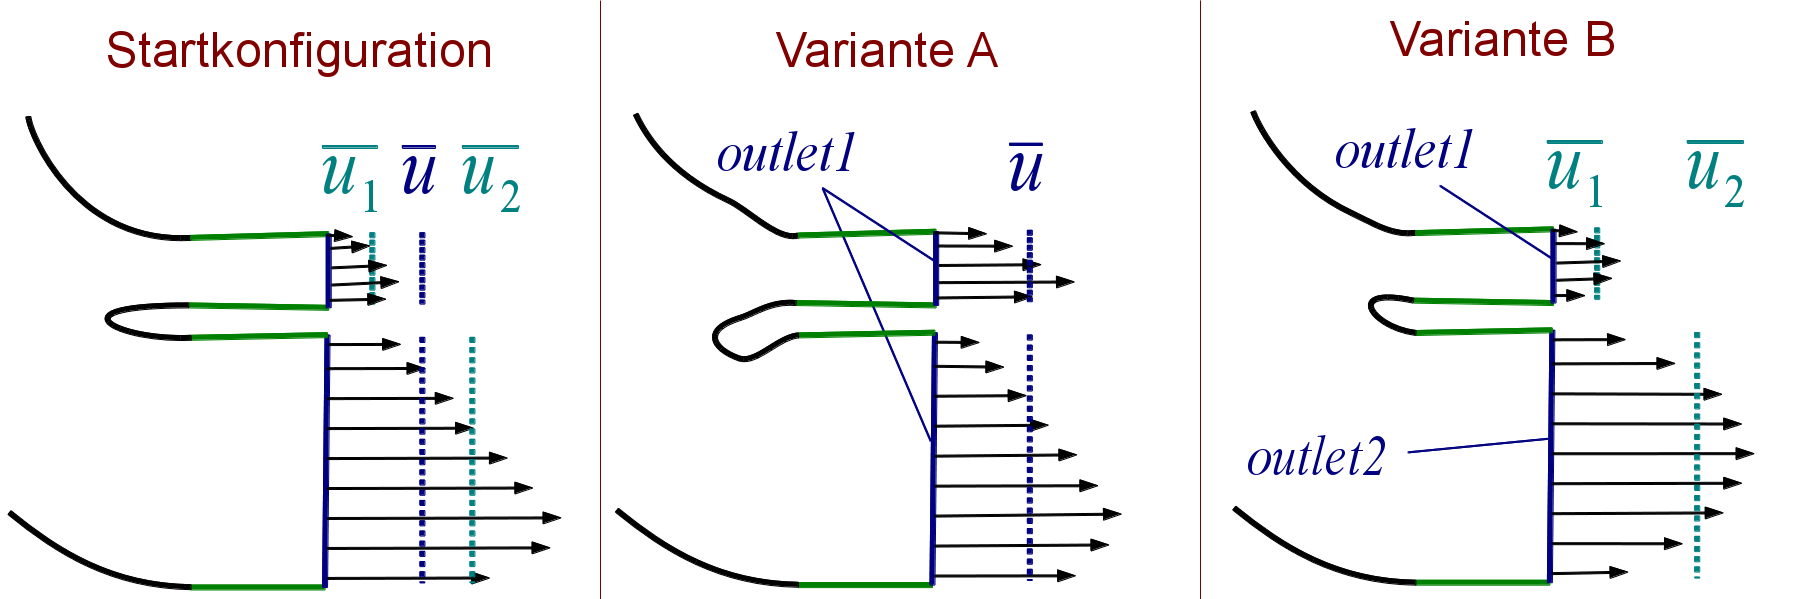
\includegraphics[scale=0.53]{outletMULT.png}   
\caption{Links: Start. Mitte: Optimierung $\JJ_1 \lvert_{ \Gamma_o^1 \cup \Gamma_o^2}$. Rechts: Optimierung $\gamma_1\JJ_1\lvert_{\Gamma_o^1} + \gamma_2 \JJ_1\lvert_{\Gamma_o^2}$. }
\label{fig:multOutlet}
\end{figure}
%
%\begin{figure}
%\begin{minipage}[b]{5.5 cm}
%Anwendungen, wie in der nebenstehenden Skizze dargestellt, können mit der aktuellen Beschränkung (3 Einströmbereiche, 3 Ausströmbereiche) gerechnet werden, sofern die Modellierungsanforderungen passen.
%$ $\\
%$ $\\
%$ $\\
%$ $\\
%\end{minipage}
%\begin{minipage}[b]{5 cm}
%\centering
%\includegraphics[scale=0.45]{skizze_designSpace8.png}   
%\end{minipage}
%\end{figure}
%%
%\newpage
\subsection{Benutzerdefiniertes Einströmprofil}
Im Falle, dass ein Einströmprofil vorgegeben werden möchte, ist der entsprechende Eintrag im Parameter \textbf{velocity\_ massflow} auf 0 zu setzen und eine Datei \textbf{velocity\_inletI.csv} mit $I=\{0,1,2,...\}$ im Order der Testrechnung anzugeben.
Möchte man im Beispiel M23 am 2. Einströmbereich ein Profil vorgegeben, so ist \textbf{velocity\_massflow} = 2(36.5, 0) zu setzen und eine Datei \textbf{velocity\_inlet2.csv} anzulegen.
\subsection{Anfangsgeometrie Topologieoptimierung}
Bei der Topologieoptimierung ist eine möglichst große Anfangsgeometrie vorzugeben.
In Abbildung \ref{AnfangTopo} ist eine Anfangsgeometrie für das Anwendungsbeispiel Reinluftrohr(RLR) dargestellt.
\begin{figure}[htbp]
\centering
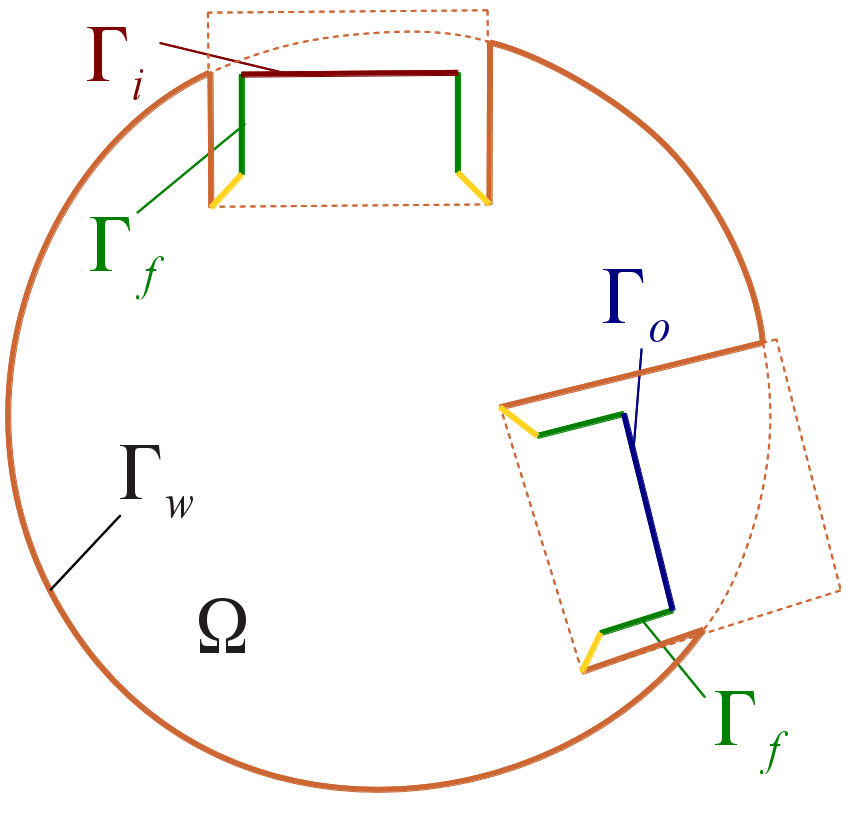
\includegraphics[scale=0.42]{TopoStartgeometrieSkizze.png}
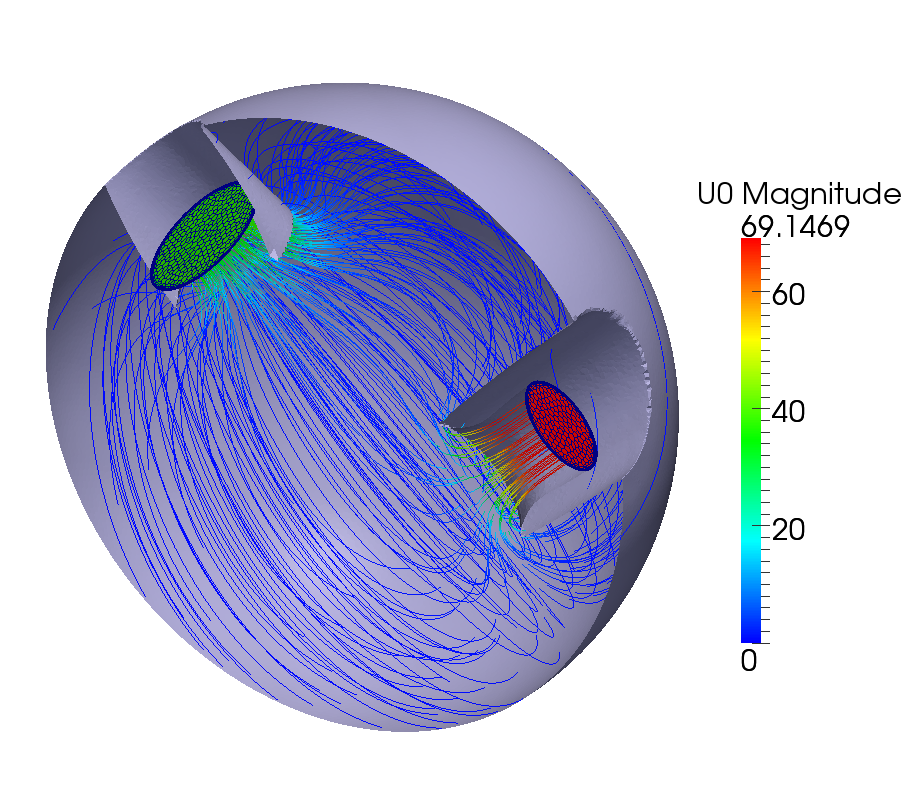
\includegraphics[scale=0.15]{TopoStartgeometrie.png}
\caption{Anfangsgeometrie Topologieoptimierung RLR.}
\label{AnfangTopo}
\end{figure}
$ $\\
\newpage
\section{Parameter und deren Bedeutung}
Neben den Geometriedaten ist die Parameterdatei \emph{parameter\_sg} anzulegen. 
Die darin enthaltenen Parameter werden in diesem Kapitel erläutert.
Die Parameter werden in den Java-Skripen \emph{mbmw3.java}, \emph{solvePrimal.java} und \emph{solveAdjoint.java} eingefügt.
Falls Änderungen in der Star-CD CCM+ Verwendung vorgenommen werden wollen, sind diese drei Dateien im Ordner \emph{initialSG} anzupassen.
Die für OpenFOAM relevanten Parameter werden nach Aufruf der Setup-Routine in \emph{system/fvSolution} gespeichert.
\begin{table}[h]
\centering
\begin{tabular}{|p{2cm}|p{1cm}|p{1.3cm}|p{0.7cm}|p{0.7cm}|p{4.6cm}|} %lcrp
\hline
\cellcolor{light-gray} Parameter-name & \cellcolor{light-gray} Default-wert 
& \cellcolor{light-gray} Zuläs-sigkeit & \cellcolor{light-gray} RLR & \cellcolor{light-gray} M23 
& \cellcolor{light-gray} Beschreibung\\
\hline
install\_ \qquad location  &        &              & & &Pfad der Star-CD CCM+ bin-Datei, um CCM+ zu starten.\\
\hline
prozessNumber       & 2  & [1,100] & 2 & 2& Prozessoranzahl bei Parallelisierung in Star-CD CCM+.\\
\hline
\end{tabular}
\caption{Parameter Star-CD CCM+.}\label{tab:parameter1}
\end{table}
\subsection{Gittererzeugung}
%
In Star-CD CCM+ wird ein Polyedergitter erzeugt.
Die Gitterfeinheit ist über den Referenzwert für die Zellengröße \textbf{base\_size} einstellbar.
Die Anzahl der In- und Outlets sowie die Anzahl der optionalen fixen Oberflächen ist anzugeben (\textbf{numInlet}, \textbf{numOutlet}, \textbf{numFixed}). 
Die Gitterqualität bei der Netzgenerierung kann über die Parameter \textbf{mesh\_opt\_cycles} und \textbf{mesh\_quality\_treshold} erhöht werden.
In Wandnähe sind Layerschichten zu verwenden, deren Größe und Anzahl durch die Parameter
 \textbf{num\_layer\_wall}, \textbf{thick\_layer} und \textbf{layer\_stretch} festgelegt sind.
Um Rückströmungen auf der Ausströmgeometrie ('do-nothing' Randbedingung) zu verhindern, ist meist eine zusätzliche Extrusionsgeometrie erforderlich.
Die Einstellung der Länge und Diskretisierung ist mit den Parametern \textbf{extrude\_...} festzulegen. 
Anhand der Oberflächenbeschaffenheit wird in CCM+ lokal das Gitter verfeinert. 
Falls diese Verfeinerung nicht durchgeführt werden soll, so ist der Parameter \textbf{grid\_local\_refinement} auf 0 zu setzen.
\begin{table}[h]
\centering
\begin{tabular}{|p{2.1cm}|p{1cm}|p{1.5cm}|p{0.6cm}|p{0.5cm}|p{0.5cm}|p{5.6cm}|} %lcrp
\hline
\cellcolor{light-gray} Parameter-name & \cellcolor{light-gray} Default-wert 
& \cellcolor{light-gray} Zuläs-sigkeit & \cellcolor{light-gray} RLR & \cellcolor{light-gray} M23 & \cellcolor{light-gray} B135
& \cellcolor{light-gray} Beschreibung\\
\hline
base\_size         & 0.004  & [1e-4,0.1]          & 0.004 & 0.03 &  0.04  & Gitterfeinheit: Zellgröße.\\
\hline
numInlet           & 1      & \{1,2,...1e3\}      & 1     &   2  &   1    & Anzahl der Einströmbereiche.\\
\hline
numOutlet          & 1      & \{1,2,...1e3\}      & 1     &   3  &   1    &   Anzahl der Ausströmbereiche.\\
\hline
numFixed           & 0      & \{0,1,...1e3\}     & 0     &   1    &   0    & Anzahl der optional fixen Geometrien.\\
\hline
num\_layer\_wall   &   2    & [0,6]              & 2     &   3    &   6    & Anzahl der Layerschichten am Rand.\\
\hline
thick\_layer       &   60   & [10,100]           & 80    &   60   & 60     & Stärke der Layerschichten in Prozent (Relativ zur Nachbarzellgröße).\\
\hline 
layer\_stretch     &   1.5  & [1e-3,1e3]         & 1.5   & 1.5    & 1.4    & Vergrößerungsfaktor d. Layerschichten.\\ 
\hline
extrude\_ \qquad \; outlet\_length & 0.05 &  [1e-8,1e8] & 0.06 & 0.2 & 1.2 & Länge der Extrusionsgeometrie am Outlet.\\
\hline
extrude\_ \qquad \; outlet\_num    & 32   &  [1,1e5]    & 20 & 10   & 90   & Anzahl der Zellschichten in der Extrusionsgeometrie am Outlet.\\
\hline
extrude\_ \qquad \; outlet\_stretch & 1   &   [1e-3,1e3]  & 1 & 1   &  1   &Vergrößerungsfaktor d. Layerschichten in d. Extrusionsgeometrie am Outlet.\\
\hline
extrude\_ \qquad \; inlet\_length   & 0.025 &   [1e-8,1e8]    & 0.03 & 0.2  & 0.2 & Länge der Extrusionsgeometrie am Inlet.\\
\hline
extrude\_ \qquad \; inlet\_num      & 16 &   [1,1e5]     & 10 & 10 & 15 & Anzahl der Zellschichten in der Extrusionsgeometrie am Inlet.\\
\hline
extrude\_ \qquad \; inlet\_stretch  & 1 &    [1e-3,1e3]      & 1 & 1 & 1 & Vergrößerungsfaktor der Layerschichten in der Extrusionsgeometrie am Inlet.\\
\hline
mesh\_opt\_ \quad cycles        & 8 &   [1,8]     & 8 & 8 & 8 & Polyedergitter: Qualitätsoptimierungsschleifen.\\
\hline
mesh\_quality \quad \_treshold  &1&   [0,1]     & 1 & 1 & 1 & Polyedergitter: Qualitätsoptimierungsschranke.\\
\hline
grid\_local\_ \qquad refinement  & 0 &  \{0,1\}    & 0 & 1 & 1 & Lokale Gitterverfeinerung: 0:nein, 1:ja.\\
\hline
ext\_merge  & 0 &  \{0,1\}    & 0 & 1 & 0 & Extrusionsgeometrie mit fixen Geometrien vereinigen: 0:nein, 1:ja.\\
\hline
\end{tabular}
\caption{Parameter für die Gittererzeugung in Star-CD CCM+.}\label{tab:parameter1}
\end{table}
%
%
%
\subsection{Modellwahl und physikalische Einstellungen}
Zur Angabe der Strömungsgeschwindigkeit kann entweder eine konstante Einströmgeschwindigkeit in m/s 
oder die Massenflussrate in kg/s angegeben werden (\textbf{velocity\_ massflow\_par} = 0 oder 1).
Die Werte sind durch den Parameter \textbf{velocity\_massflow} anzugeben.
Die entsprechende Syntax ist der Tabelle \ref{tab:parameter2a} zu entnehmen.\\ 
%Optional kann ein poröses Medium verwendet werden (\textbf{porous\_medium}).
%Die Impulsgleichung im porösen Medium lautet:
%\begin{equation}
% \nabla \cdot \left(\buu \buu^{T} \right) -\nu \Delta \buu + \nabla p \, \, \textcolor{blue}{ + \, P_V \buu + P_I \left| \buu \right| \buu } = \bzz,
%\end{equation}
%%
%wobei der Zähigkeits- bzw. der Trägheitsanteil in Star-CD CCM+ 
%als Diagonalmatrix $P_V$ bzw. $P_I$ anzugeben ist.
%\begin{itemize}
%\item Porous Inertial (Trägheit) Resistence Tensor $P_I=\left(\begin{matrix}  
% \textbf{PIRxx} & & 0 \\  & \textbf{PIRyy} & \\ 0 & & \textbf{PIRzz}
% \end{matrix}\right)$.
%\item Porous Viscous (Zähigkeit) Resistence Tensor $P_V=\left(\begin{matrix}  
% \textbf{PVRxx} & & 0 \\  & \textbf{PVRyy} & \\ 0 & & \textbf{PVRzz}
% \end{matrix}\right)$.
%\end{itemize}
%%
%%
\begin{table}[h]
\centering
\begin{tabular}{|p{2.8cm}|p{0.9cm}|p{1.5cm}|p{0.8cm}|p{1.0cm}|p{0.7cm}|p{4.3cm}|} %lcrp
\hline
\cellcolor{light-gray} Parametername & \cellcolor{light-gray} Default-wert & \cellcolor{light-gray} Zuläs-sigkeit & \cellcolor{light-gray} RLR & \cellcolor{light-gray} M23  & \cellcolor{light-gray} B135 & \cellcolor{light-gray} Beschreibung\\
\hline
turb\_model                     &   2           & [0,100]      & 1      & 0               &  4  & 0: DNS, 1: Realiz. k-$\varepsilon$ all Y+, 2: Std. k-$\varepsilon$ high Y+, 3: RSM all Y+, 4: Realiz. k-$\varepsilon$ low Y+.\\
\hline
velocity\_massflow\_ \quad par  &   0           & \{0,1\}      & 0      & 0               &  0  & Einströmung: 0:Geschwindigkeit, 1:Massenstrom.\\
\hline
velocity\_massflow              &  1(0.1)       &  [1e-8,1e8]  & 1(36.5)& 2(0.006, 0.006) &  1(4.3)  & Einströmung (Geschwindigkeit bzw. Massenstrom)\\
\hline
inlet\_turb\_intensity          &  0.1          &  [1e-8,1e8]  & 0.1    &                 &  0.1  & Turbulent Intensity Inlet.\\
\hline
inlet\_turb\_length    &   \textcolor{dred}{10} &  [1e-8,1e8]   & 0.1   &                 &   10 & Turbulent Length Scale Inlet.\\
\hline
outlet\_turb\_intensity        &  0.1           &  [1e-8,1e8]   & 0.1   &                 &   0.1 & Turbulent Intensity Outlet.\\
\hline
outlet\_turb\_length      & \textcolor{dred}{10} &  [1e-8,1e8]  & 0.1   &                 &   10 & Turbulent Length Scale Outlet.\\
\hline
\end{tabular}
\caption{Parameter zu Physikalischen Modellen.}\label{tab:parameter2a}
\end{table}
%\begin{table}[h]
%\centering
%\begin{tabular}{|p{2.8cm}|p{1cm}|p{1.5cm}|p{0.6cm}|p{1.1cm}|p{5.1cm}|} %lcrp
%\hline
%\cellcolor{light-gray} Parametername & \cellcolor{light-gray} Default-wert & \cellcolor{light-gray} Zuläs-sigkeit & \cellcolor{light-gray} RLR & \cellcolor{light-gray} F3 & \cellcolor{light-gray} Beschreibung\\
%\hline
%porous\_medium  &   0   &  \{0,1\} & 0 & 1 & Poröses M.: 0:nein, 1:ja.\\
%\hline
%porous\_turb\_ \quad \; intensity  &  0.1  & [1e-8,1e8]   & 0.1 & 0.1  &Turbulent Intensity Porous Medium.\\
%\hline
%porous\_turb\_ \quad length      &  \color{dred}{10}  &  [1e-8,1e8]  & 10 & 10 & Turbulent Length Scale Porous Medium.\\
%\hline
%PIR\_xxAxis0      &   0   &  [-1e8,1e8]  &  0  & 0.0053  & PIR.: X-Achse, 1.Komponente.\\
%\hline
%PIR\_xxAxis1      &   0   &  [-1e8,1e8]  &  0  & 0.99996 & PIR.: X-Achse, 2.Komponente.\\
%\hline
%PIR\_xxAxis2      &   0   &  [-1e8,1e8]  &  0  & 0.0     & PIR.: X-Achse, 3.Komponente.\\
%\hline
%PIR\_yyAxis0      &   0   &  [-1e8,1e8]  &  0  & 0.99996 & PIR.: Y-Achse, 1.Komponente.\\
%\hline
%PIR\_yyAxis1      &   0   &  [-1e8,1e8]  &  0  & -0.0053 & PIR.: Y-Achse, 2.Komponente.\\
%\hline
%PIR\_yyAxis2      &   0   &  [-1e8,1e8]  &  0  & -0.0077 & PIR.: Y-Achse, 3.Komponente.\\
%\hline
%PVR\_xxAxis0      &   0   &  [-1e8,1e8]  &  0  & 0.0053  & PVR.: X-Achse, 1.Komponente.\\
%\hline
%PVR\_xxAxis1      &   0   &  [-1e8,1e8]  &  0  & 0.99996 & PVR.: X-Achse, 2.Komponente.\\
%\hline
%PVR\_xxAxis2      &   0   &  [-1e8,1e8]  &  0  & 0.0     & PVR.: X-Achse, 3.Komponente.\\
%\hline
%PVR\_yyAxis0      &   0   &  [-1e8,1e8]  &  0  & 0.99996 & PVR.: Y-Achse, 1.Komponente.\\
%\hline
%PVR\_yyAxis1      &   0   &  [-1e8,1e8]  &  0  & -0.0053 & PVR.: Y-Achse, 2.Komponente.\\
%\hline
%PVR\_yyAxis2      &   0   &  [-1e8,1e8]  &  0  & -0.0077 & PVR.: Y-Achse, 3.Komponente.\\
%\hline
%PIR\_xxComponent  &   0   &  [-1e8,1e8]  &  0  & 10000 & Poröses M.: X-Trägheitsanteil.\\
%\hline
%PIR\_yyComponent  &   0   &  [-1e8,1e8]  &  0  & 11.12 & Poröses M.: Y-Trägheitsanteil.\\
%\hline
%PIR\_zzComponent  &   0   &  [-1e8,1e8]  &  0  & 1000  & Poröses M.: Z-Trägheitsanteil.\\
%\hline
%PVR\_xxComponent  &   0   &  [-1e8,1e8]  &  0  & 100000 & Poröses M.: X-Zähigkeitsanteil.\\
%\hline
%PVR\_yyComponent  &   0   &  [-1e8,1e8]  &  0  & 1560.0 & Poröses M.: Y-Zähigkeitsanteil.\\
%\hline
%PVR\_zzComponent  &   0   &  [-1e8,1e8]  &  0  & 100000 & Poröses M.: Z-Zähigkeitsanteil.\\
%\hline
%%viscosity*      &   0   &  1  &   & 2e-4 & Viskosität (nur falls ccm\_solver=0).\\
%%\hline
%\end{tabular}
%\caption{Parameter zu Physikalischen Modellen: Poröses Medium.}\label{tab:parameter2b}
%\end{table}
%Das Koordinatensystem muss entsprechend festgelegt werden. 
%Dazu ist die Hauptdurchlaufrichtung als Richtung der Y-Achse ( \textbf{YA1}, \textbf{YA2}, \textbf{YA3} ) anzugeben. 
%Eine Richtung orthogonal zur Durchlaufrichtung wird als Richtung der X-Achse ( \textbf{XA1}, \textbf{XA2}, \textbf{XA3} ) angegeben. 
%Zwei der in Star-CD CCM+ vorkommenden Turbulenzmodelle, welche sich bei Verwendung mit der adjungierten Gleichung als geeignet erwiesen haben, können mit dem Parameter \textbf{stdKE\_relKE} gewählt werden.
Neben der Direkten Numerischen Simulation (\textbf{turb\_model} = 0) können derzeit 4 Turbulenzmodelle mit dem Parameter \textbf{turb\_model} gewählt werden.
Falls sich bei künftigen Softwareversionen andere Turbulenzmodelle als geeignet erweisen, so ist das Java-Skript \emph{mbmw3.java} entsprechend anzupassen.
Weiters sind folgende Modell- Kenngrößen in Star-CD CCM+ anzugeben: % die als Startwerte für das Erstellen der Randbedingungen für die $k$ - Epsilon Gleichungen dienen. 
\textbf{inlet\_turb\_intensity}, \textbf{inlet\_visc\_ratio}, \textbf{outlet\_ turb\_intensity}, 
\textbf{outlet\_visc\_ratio}.\\
\subsection{Lösereinstellungen für die primale und adjungierte Gleichung}
Bei den Lösern in CCM+ wird ein pseudo-Zeitschrittverfahren verwendet. 
Die Schrittweitensteuerung ist über die Courant-Friedrichs-Lewy-Zahl (\textbf{CFLpri}, \textbf{CFLadj}) anzugeben.
Die Wahl einer großen Zahl ermöglicht ein schnelleres Erzielen der gewünschten Lösung, kann jedoch bei zu großer Wahl zu Konvergenzproblemen führen.
Für die adjungierte Gleichung steht neben dem Standardlöser auch ein GMRES Löser zur Verfügung (\textbf{gmresAdj}) 
mit den relevanten Einstellungen \textbf{krylov\_dim, krylov\_accuracy}.\\
$ $\\
Als Abbruchkriterien werden die maximale Anzahl an Iterationen (\textbf{iterPri}, \textbf{iterAdj}) und ein Abbruch bei gewünschten Genauigkeiten verwendet.
Zweiteres ist erzielt, wenn die Standardabweichung jeweils unter den Toleranzwerten (\textbf{stop\_accuracyPri},\\ \textbf{stop\_accuracyAdj}) liegt. 
Wählt man \textbf{stop\_sample} z.B. 100, so wird stets die Standardabweichung der letzten 100 Iterationen berechnet.\\
$ $\\
Der primale Löser gilt als auskonvergiert, wenn die gewünschte Lösungsgenauigkeit vor erreichen der Iteration \textbf{iterPri} erzielt wird.
Ist die Genauigkeit nach \textbf{iterPri} Schritten nicht erreicht, so wird bei der Gitterverschiebung eine kleinere Schrittweite gewählt.
Wichtig ist daher stets sicherzustellen, dass \textbf{iterPri} groß genug gewählt wird!\\
$ $\\
Falls es zu Konvergenzproblemen des adjungierten Lösers kommt, so ist der Parameter \textbf{adj\_order} auf 1 zu setzen.
%
%
\begin{table}[h]
\centering
%\begin{tabular}{|p{2.5cm}|p{1.1cm}|p{1.8cm}|p{1cm}|p{4cm}|} %lcrp
%\hline
%\cellcolor{light-gray} Parametername & \cellcolor{light-gray} Default-wert & \cellcolor{light-gray} Zulässigkeit & \cellcolor{light-gray} RLR  & \cellcolor{light-gray} Beschreibung\\
%\hline
\begin{tabular}{|p{2.4cm}|p{1cm}|p{0.9cm}|p{0.9cm}|p{1.1cm}|p{0.9cm}|p{4.8cm}|} %lcrp
\hline
\cellcolor{light-gray} Parameter- \quad name & \cellcolor{light-gray} Default-wert & \cellcolor{light-gray} Zuläs-sigkeit & \cellcolor{light-gray} RLR & \cellcolor{light-gray} M23 & \cellcolor{light-gray} B135 & \cellcolor{light-gray} Beschreibung\\
\hline
ccm\_solver   &   1   & \{0,1\} & 1   & 1 & 1 & 1: Verwendung von CCM+ Löser, 0: Alternative Löser.\\
\hline
gmresAdj     &   0   & \{0,1\} & 0   & 0 &  0 & Adjungierter Löser: 0: ohne GMRES, 1: mit GMRES.\\
\hline
krylov\_dim  &   50   &   [1,1e5]   &    &   &   & Anzahl der Krylovräume (adj, GMRES).\\
\hline
krylov\_accuracy & 1e-12 &  ]0,1]   &    &   &   & Rechengenauigkeit Krylovräume.\\
\hline
CFLpri       &   4   &   [0.1, 1000]   & 4   & 3 & 4 & CFL primal.\\
\hline
CFLadj       &   100   &   [0.1, 10000]    & 90  & 40 & 90 & CFL adjoint.\\
\hline
stop\_accuracyPri & 1e-12 & ]0,1]  & 1e-12 & 1e-12 & 1e-8 & Abbruchkriterium Standardabweichung: Genauigkeit primale Lösung.\\
\hline
stop\_accuracyAdj & 1e-12 & ]0,1]  & 1e-12 & 1e-12 & 1e-12 & Abbruchkriterium Standardabweichung: Genauigkeit adjungierte Lösung.\\
\hline
stop\_sample  &  100  &   [1,1e5]  & 200  & 50 & 50 & Abbruchkriterium Standardabweichung: Anzahl der zu betrachtenden Iterationen.\\
\hline
iterPri      &   2000   &  [1,1e4] & 4000 & 2500 & 1200 & Maximale Iterationszahl der primalen Gleichung nach einem Remeshing.\\
\hline
iterAdj      &   1000   &  [1,1e5] & 3000 & 2000 & 1000 & Maximale Iterationszahl der adjungierten Gleichung nach einem Remeshing.\\
\hline
adj\_order     &   2   & \{1,2\} & 2   & 2 &  1  & Diskretisierung Adjungierte Ordnung.\\
\hline
\end{tabular}
\caption{Parameter für die Löser in Star-CD CCM+.}\label{tab:parameter3}
\end{table}
%
\newpage
\subsection{Liniensuche}
Im Zuge der Formoptimierung verwenden wir eine Schrittweitensteuerung basierend auf der Gitterqualitätsabfrage 
und der Abfrage nach einer hinreichend großen Reduktion des Funktionswertes. 
Die verwendete Regel nennt sich \emph{Armijo line search} und lautet:  
\begin{equation}
\label{armijo1}\JJ_{12}^\alpha \left( \Om^{k+1} \right) \leq \JJ_{12}^\alpha \left( \Om^{k} \right) - \mu s_k \lVert \DD \JJ_{12}^\alpha \left( \Om^{k}  \right) \rVert_{L^2\left(\Gamma_w^k\right)} 
%\label{armijo1}\JJ_{12}^\alpha \left( \buu\left(\Om^{k+1} \right) \right) \leq \JJ_{12}^\alpha \left( \buu \left( \Om^{k} \right) \right) - \mu s_k \lvert \partial \JJ_{12}^\alpha \left( \buu \left(\Om^{k} \right); V \right) \rvert 
\end{equation}
mit $0<\mu<1$ und $\Om^{k+1}=\T_{D\left(s_k, \Om^k\right)} \left(\Om^k\right)$. 
Die Abbildung $\T_{D\left(s_k, \Om^k\right)\left(\Om\right)\left(\bxx\right)}$:$\RR^3 \rightarrow \RR^3$ wird anhand des Formgradienten bestimmt.\\
$ $\\
Vom Benutzer ist eine Startschrittweite $s_0$ (\textbf{spStepLength}) anzugeben.
Im Falle, dass die Bedingung \eqref{armijo1} nicht erfüllt ist, wird die Schrittweite um den Faktor \textbf{spReduceKoeff} verkleinert.
Die Reduktion der Schrittweite wird so lange durchgeführt, bis die Schrittweite kleiner ist als der Wert \textbf{spLowerBound}.
Danach erfolgt eine Gitterneuvernetzung.
Die Gewichtung $\mu>0$ (\textbf{linesearchGewicht}) sichert einen hinreichend großen Abstieg, welcher für die mathematische Betrachtung der Liniensuche relevant ist. 
Für die numerische Anwendung sollte dieser Parameter eher klein gesetzt werden. 
Falls man eine Gitterneuvernetzung nach einer gewissen Anzahl an Iterationen erzwingen möchte, kann dies mit dem Parameter \textbf{remesh\_iter} erfolgen.
Üblicherweise ist eine Gitterneuvernetzung bei zulässigem Gitter nicht erforderlich.
Somit wurde dieser Wert bei den Berechnungen größer als die maximale Iterationszahl gesetzt.
\begin{table}[h]
\centering
%\begin{tabular}{|p{2.5cm}|p{1.1cm}|p{1.8cm}|p{1cm}|p{4cm}|} %lcrp
%\hline
\begin{tabular}{|p{2.4cm}|p{1.1cm}|p{0.8cm}|p{0.9cm}|p{0.9cm}|p{4cm}|} %lcrp
\hline
\cellcolor{light-gray} Parametername & \cellcolor{light-gray} Default-wert & \cellcolor{light-gray} Zuläs-sigkeit & \cellcolor{light-gray} RLR & \cellcolor{light-gray} M23 & \cellcolor{light-gray} Beschreibung\\
%\hline
%\cellcolor{light-gray} Parametername & \cellcolor{light-gray} Default-wert & \cellcolor{light-gray} Zulässigkeits-bereich & \cellcolor{light-gray} RLR  & \cellcolor{light-gray} Beschreibung\\
\hline
spStepLength      &   2.0e-6 & [0,1]     & 1e-4 & 1e-2 & Startschrittweite $s_0$ in der Armijo Liniensuche \ref{armijo1}. \\
\hline
spLowerBound      &   1.0e-8 & [0,1]     & 1e-6 & 1e-5 & Untere Schranke der Schrittweite.\\
\hline
spReduceKoeff     &   0.5    & [0,1]     & 0.6  & 0.5 & Reduktionsfaktor bei Schrittweitensteuerung.\\
\hline
linesearchGewicht &  1.0e-16 & [0,1]     & 1e-14 & 0  & Gewichtung $\mu$ in Armijo-Liniensuche.\\
\hline
remesh\_iter      &   1000   & [1,1e5]   & 900   & 10 & Remeshing in jeder ... ten Iteration erzwingen (auch wenn Gitterqualität OK).\\
\hline
\end{tabular}
\caption{Parameter zur Liniensuche in OpenFOAM.}\label{tab:parameter4}
\end{table}
%
\subsection{Abbruchkriterien der Formoptimierung}
In Tabelle \ref{tab:abbruch} sind die Parameter zur Beendigung der Formoptimierung angegeben.
Am relevantesten dafür sind maximale Anzahl an Iterationen (\textbf{outerLoopEnd}), die Anzahl an durchgeführten Remeshings (\textbf{rem\_max}) und der Fortschritt im Zielfunktional (\textbf{sigma\_stop\_J}). 
\begin{table}[h]
\centering
%\begin{tabular}{|p{2.5cm}|p{1.1cm}|p{1.8cm}|p{1cm}|p{4cm}|} %lcrp
%\hline
%\cellcolor{light-gray} Parametername & \cellcolor{light-gray} Default-wert & \cellcolor{light-gray} Zulässigkeits-bereich & \cellcolor{light-gray} RLR  & \cellcolor{light-gray} Beschreibung\\
\begin{tabular}{|p{2.6cm}|p{1cm}|p{1.4cm}|p{0.7cm}|p{0.7cm}|p{4cm}|} %lcrp
\hline
\cellcolor{light-gray} Parametername & \cellcolor{light-gray} Default-wert & \cellcolor{light-gray} Zuläs-sigkeit & \cellcolor{light-gray} RLR & \cellcolor{light-gray} M23 & \cellcolor{light-gray} Beschreibung\\
\hline
outerLoopEnd      &   8      & [1,1e5]   & 200   & 200 & Maximale Anzahl an Iterationen.\\
\hline
%outerLoopCycleNr  &   1      & [1,1e5]   & 1     & 1 & Anzahl wie oft $\alpha$ reduziert/vergrößert wird.\\
%\hline
rem\_max          &   20     & [1,1000]  & 30    & 30 & Maximale Anzahl an durchgeführten Remeshings.\\
\hline
rem\_num\_max     &   8      & [1,1000]  & 30    & 30 & Maximale Anzahl an Remeshings mit rem\_tol Abstand.\\
\hline
rem\_tol          &   2      & [0,100]   & 2     &    & Abstandstoleranz bei Remeshing.\\
\hline
sigma\_stop\_J    &   50     & [0,100]   & 100   & 100 & Abbruchkriterium: Fortschritt in \% im Zielfunktional J. Notation: $\sigma$.\\
\hline
sigma\_stop\_DJ   &   50     & [0,100]   & 100   & 100 & Abbruchkriterium: Fortschritt in \% in der L2-Norm des Formgradienten. Notation: $\sigma_d$.\\
\hline
%kruemmNTol   &   1e5   & [1,1e8]   & 1e5   & 1e5 & Abbruchkriterium: Oberflächenkrümmung.\\
%\hline
%kruemmTol   &   20     & [0.001,1e8]   & 20   & 20 & Abbruchkriterium: Oberflächenkrümmung.\\
%\hline
\end{tabular}
\caption{Abbruchkriterien der Formoptimierung in OpenFOAM.}\label{tab:abbruch}
\end{table}
%
%
%\newpage
\subsection{Formoptimierung: Zielfunktionale.}
\subsubsection{Gleichmäßige Ausströmung und Totaldruckverlust}
Die Formoptimierung kann hinsichtlich des Erzielens einer gleichmäßigen Ausströmung und der Minimierung des Totaldruckverlustes durchgeführt werden. 
Das diskrete Zielfunktional hinsichtlich gleichmäßiger Ausströmung lautet:
\begin{equation}
\label{J1} \JJ_1= \frac{ \sqrt{ \frac{1}{A}\underset{k \in \Gamma_o}{\sum} \left(\buu_k\cdot \bnn_k - \bu \right)^2 A_k}}{\bu}\\
\end{equation}
mit 
\begin{equation}
\bu= \frac{1}{A} \underset{j \in \Gamma_o}{\sum} \buu_j \cdot \bnn_j A_j,
\end{equation}
wobei $A=\left|\Gamma_o\right|$.
Das diskrete Zielfunktional hinsichtlich Minimierung des Totaldruckverlustes lautet:
\begin{equation}
 \JJ_2= \left| \frac{\underset{k \in \Gamma_i}{\sum}\left(p_k+\frac{\rho_k}{2}\left(\buu_k \cdot \buu_k \right)\right) \buu_k \cdot \left(-\bnn_k\right) \; A_k}{\underset{k \in \Gamma_i}{\sum} \buu_k \cdot \left(-\bnn_k\right) A_k}\right|
     -\left| \frac{\underset{k \in \Gamma_o}{\sum}\left(p_k+\frac{\rho_k}{2}\left(\buu_k \cdot \buu_k \right)\right) \buu_k \cdot \bnn_k \; A_k}{\underset{k \in \Gamma_o}{\sum} \buu_k \cdot \bnn_k A_k}\right|.
\end{equation}
Wir bezeichnen mit $\buu_k$ den Geschwindigkeitsvektor an der finiten Fläche mit Index $k$.
Der Druck $p_k$ und die Dichte $\rho_k$ wird ebenfalls jeweils an der finiten Fläche mit Index $k$ ausgewertet. 
Um die Notation einfach zu halten, bezeichnen wir die Indexmenge aller Flächenstücke an der Einströmgeometrie bzw. Ausströmgeometrie mit $\Gamma_i$ bzw. $\Gamma_o$. 
Das Oberflächenmaß einer finiten Fläche ist mit $A_k$ bezeichnet. 
Der nach außen gerichtete Einheitsnormalvektor wird mit $\bnn_k$ bezeichnet.
Der Einheitsnormalvektor $\bnn_k$ auf $\Gamma_i$ ist gegen die Hauptströmungsrichtung orientiert. 
Daraus ergibt sich das gemischte Zielfunktional:
 \begin{equation}
\label{2.1} \JJ_{12}\left( \buu \left( \Om \right) \right)  = \left(1-\gamma \right)\JJ_1 \left( \buu \left( \Om \right) \right) + \gamma \rho \JJ_2 \left( \buu \left( \Om \right) \right)
\end{equation}
\begin{equation*}
\mbox{mit} \quad \gamma \in \left[0,1\right] \quad \mbox{und} \quad \rho = \begin{cases}
        \frac{\left\Vert\partial \JJ_1 \left(\buu \left( \Om^0 \right) \right) \right\Vert_{L^2\left(\Gamma_w^0\right)}}{\left\Vert\partial \JJ_2\left(\buu \left(\Om^0 \right) \right) \right\Vert_{L^2\left(\Gamma_w^0\right)}} & \mbox{wenn } \gamma \in \left(0,1\right),\\ 
        1 & \mbox{wenn } \gamma \in \{ 0, 1 \},
       \end{cases}
\end{equation*}
mit dem Gewichtungsparameter $\gamma$ ($\textbf{dp\_J12}$).
%Anstelle der Verwendung von $\Gamma_i$ und $\Gamma_o$ in den Zielfunktionalen, können optional auch die Oberflächen $\overline{\Gamma_i}$ und $\overline{\Gamma_o}$ herangezogen werden (siehe Abbildung \ref{Skizze_extrusion}).
%Hierzu ist der Parameterwert \textbf{interface\_fv} entsprechend zu setzen.\\
\begin{figure}[htbp]
\centering
    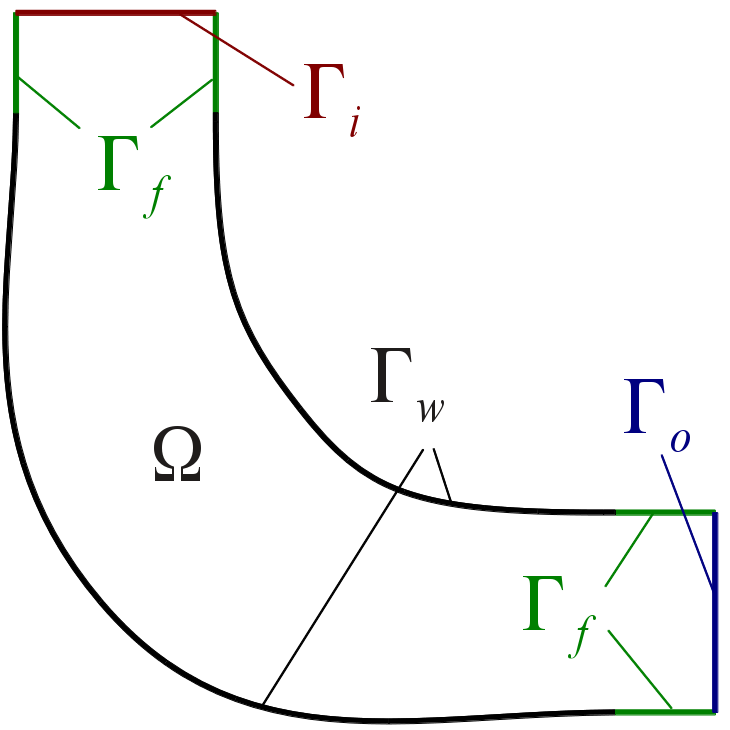
\includegraphics[scale=0.5]{geometrie_skizze_noInterface.png}
    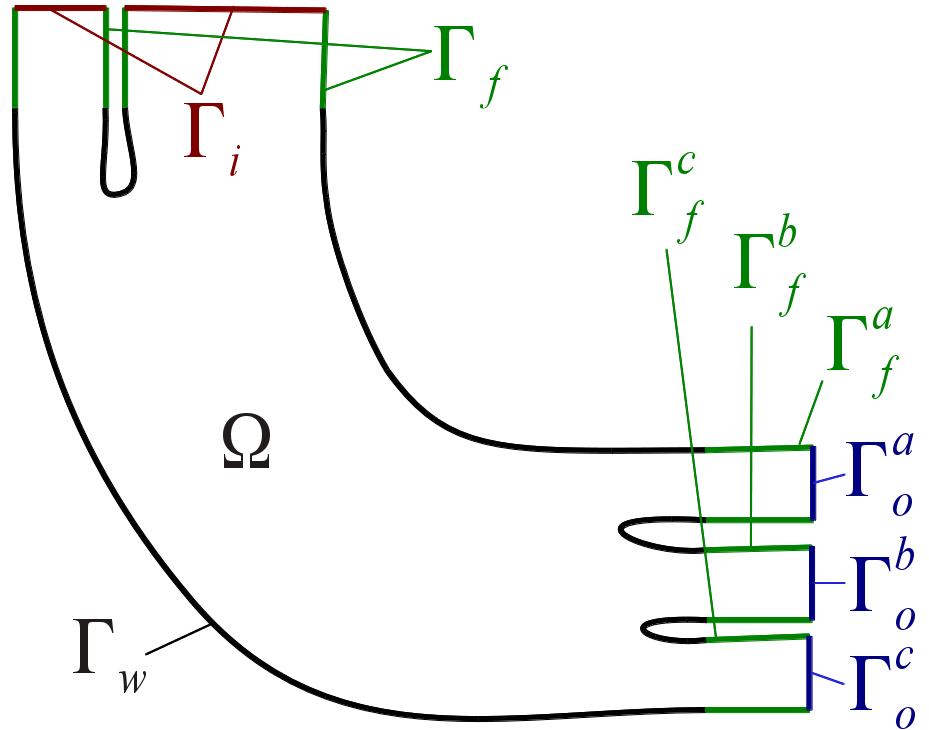
\includegraphics[scale=0.5]{geometrie_skizze_MultOutlet.png}
\caption{Skizze von $\Om$ mit Bezeichnung der Teile der Oberfläche.}
\label{Skizze_extrusion}
\end{figure}
Die Parameter \textbf{gnu\_plot\_visual} und \textbf{gnu\_plot\_visual\_i} dienen zur grafischen Darstellung der Zielfunktionswerte.
Falls diese Option gewählt wird, erscheinen die Grafiken während der Formoptimierung und werden im Testlauf-Ordner unter 
\emph{Funktionswerte\_J1.ps}, \emph{Funktionswerte\_J2.ps} und \emph{Funktionswerte\_J12.ps} gespeichert. 
%Falls zur Berechnung der Formsensitivität anstelle der äußersten Randschicht, Randschichten weiter innerhalb der Geometrie verwendet werden sollen, ist der Parameter \textbf{sg\_layer} zu verwenden (siehe Abbildung \ref{Filter5}).
%\begin{figure}[htbp]
%    \begin{minipage}[b]{6 cm}
%    \includegraphics[scale=0.13]{filter_layer.png}
%  \end{minipage}
%  \begin{minipage}[b]{4 cm}
%    \includegraphics[scale=0.8]{skizze_filter_layer2.png}
%  \end{minipage}
%  \caption{Layerstruktur der Geometrie in Wandnähe: links: F3 Ausschnitt, rechts: Skizze.}
%  \label{Filter5}
%\end{figure}
%
%
\begin{table}[h]
\centering
%\begin{tabular}{|p{2.5cm}|p{1.1cm}|p{1.8cm}|p{1cm}|p{4cm}|} %lcrp
%\hline
%\cellcolor{light-gray} Parametername & \cellcolor{light-gray} Default-wert & \cellcolor{light-gray} Zulässigkeits-bereich & \cellcolor{light-gray} RLR  & \cellcolor{light-gray} Beschreibung\\
\begin{tabular}{|p{2.5cm}|p{1cm}|p{1.6cm}|p{0.6cm}|p{1.3cm}|p{4cm}|} %lcrp
\hline
\cellcolor{light-gray} Parametername & \cellcolor{light-gray} Default-wert & \cellcolor{light-gray} Zuläs-sigkeit & \cellcolor{light-gray} RLR & \cellcolor{light-gray} M23 & \cellcolor{light-gray} Beschreibung\\
\hline
dp\_J12              &  0.5    & [0,1]    & 0.5   & 0.5 & Gewichtungsparameter $\gamma$ zwischen $\JJ_1$ und $\JJ_2$.\\
\hline
dp\_J1              &  1(0)    & $\sum$ dp\_J1 $\in$ [0,1]    & 1(0)   & 3(0.25, 0.25,0.25) & Gewichtungsparameter $\gamma_i$ betreffend $\JJ_{1}$.\\
\hline
%interface\_fv        &  0      & \{0,1\}  & 0     & 0 & Zielfunktionen auf $\Gamma_i$, $\Gamma_o$ (0) oder Zielfunktionen auf $\overline{\Gamma_i}$, $\overline{\Gamma_o}$ (1).\\
%\hline
gnu\_plot\_visual    &  0      & \{0,1\}  & 0     & 0 & Grafische Darstellung der Zielfunktionswerte (1). Keine grafische Darstellung (0).\\
\hline
gnu\_plot\_visual\_i &  3      & [1,1000] & 1     & 1 & Aktualisieren der Grafiken nach ... Iterationen.\\      
%\hline
%sg\_layer            &  0      & [0,100]  & 0     & 1 & 0: Äußerste Randschicht für Formsensitivität; 1,2,...100: innere Randschichten.\\
\hline
\end{tabular}
\caption{Formoptimierung: Zielfunktionale}\label{tab:parameter4}
\end{table}
%
\subsubsection{Zielfunktionale bei mehreren Ausströmbereichen}
Zur Veranschaulichung verwenden wir 3 Aussrömbereiche und bezeichnen diese mit $\Gamma_o^a, \Gamma_o^b, \Gamma_o^c$.
Die Zielfunktionale für die gleichmäßige Ausströmung lauten:
\begin{eqnarray}
\JJ_{1}=\JJ_{1}\lvert_{\Gamma_o^a \cup \Gamma_o^b \cup \Gamma_o^c },\quad
\JJ_{1a}=\JJ_{1}\lvert_{\Gamma_o^a },\quad
\JJ_{1b}=\JJ_{1}\lvert_{\Gamma_o^b },\quad
\JJ_{1c}=\JJ_{1}\lvert_{\Gamma_o^c }.
\end{eqnarray}
Das gemischte Zielfunktional lautet:
\begin{eqnarray}
\JJ_{12}&=&\left(1-\gamma\right)\left(1-\gamma_a -\gamma_b -\gamma_c\right) \rho_1 \JJ_1 \\
& & + \left(1-\gamma\right) \gamma_a \rho_{1a} \JJ_{1a} + \left(1-\gamma\right) \gamma_b \rho_{1b} \JJ_{1b} + \left(1-\gamma\right) \gamma_c \rho_{1c} \JJ_{1c} \\
& & + \gamma \rho_2 \JJ_2
\end{eqnarray}
mit den, vom Benutzer vorgegebenen, Gewichtungsparametern $\gamma, \gamma_{a}, \gamma_{b}, \gamma_{c} \in \left[ 0,1\right]$ (\textbf{dp\_J12}, \textbf{dp\_J1}) wobei $\gamma_{a} + \gamma_{b} + \gamma_{c} \leqslant 1$ zu gelten hat und den 
Skalierungen $\rho_1$, $\rho_2$, $\rho_{1a}$, $\rho_{1b}$, $\rho_{1c}$, die sich folgendermaßen berechnen falls $\gamma<1$.
%
Wir definieren
\begin{eqnarray}
\mu_{uni}= max \left(\;  
\hat{\gamma_1}\left\Vert\partial \JJ_1 \left(\buu \left( \Om^0 \right) \right) \right\Vert_{L^2\left(\Gamma_w^0\right)} \; , \; 
\hat{\gamma_a}\left\Vert\partial \JJ_{1a} \left(\buu \left( \Om^0 \right) \right) \right\Vert_{L^2\left(\Gamma_w^0\right)} \; , \right.\\
\left.\hat{\gamma_b}\left\Vert\partial \JJ_{1b} \left(\buu \left( \Om^0 \right) \right) \right\Vert_{L^2\left(\Gamma_w^0\right)}\; , \;
\hat{\gamma_c}\left\Vert\partial \JJ_{1c} \left(\buu \left( \Om^0 \right) \right) \right\Vert_{L^2\left(\Gamma_w^0 \; \right)}
\right)
\end{eqnarray}
wobei wobei $\Om^0$ und $\Gamma_w^0$ die Geometrie im Gebiet und am Rand zu Beginn der Formoptimierung ist und
\begin{eqnarray}
\hat{\gamma_1} = \begin{cases} 0 & \mbox{wenn} \, \gamma_a+\gamma_b+\gamma_c =1,\\
1 & \mbox{wenn} \, \gamma_a+\gamma_b+\gamma_c <1,
\end{cases}\;
\hat{\gamma_I} = \begin{cases} 0 & \mbox{wenn} \, \gamma_I = 0,\\
1 & \mbox{wenn} \, \gamma_I > 0,
\end{cases}
\mbox{mit} \, I \in \{ a, b, c \}. \;
%\hat{\gamma_b} = \begin{cases} 0 & \mbox{wenn} \; \gamma_b = 0,\\
%1 & \mbox{wenn} \; \gamma_b > 0,
%\end{cases}
%\hat{\gamma_c} = \begin{cases} 0 & \mbox{wenn} \; \gamma_c = 0,\\
%1 & \mbox{wenn} \; \gamma_c > 0.
%\end{cases}
\end{eqnarray}
%
Die Skalierungsparameter lauten
\begin{eqnarray}
\rho_k = \frac{\mu_{uni}}{\left\Vert\partial \JJ_k \left(\buu \left( \Om^0 \right) \right) \right\Vert_{L^2\left(\Gamma_w^0\right)}} \; \mbox{mit} \; k \in \{1,2,1a,1b,1c\}.
\end{eqnarray}
Falls $\gamma=1$, so ist $\rho_1=1$ gesetzt.
%
%\begin{figure}[htbp]
%\centering
%    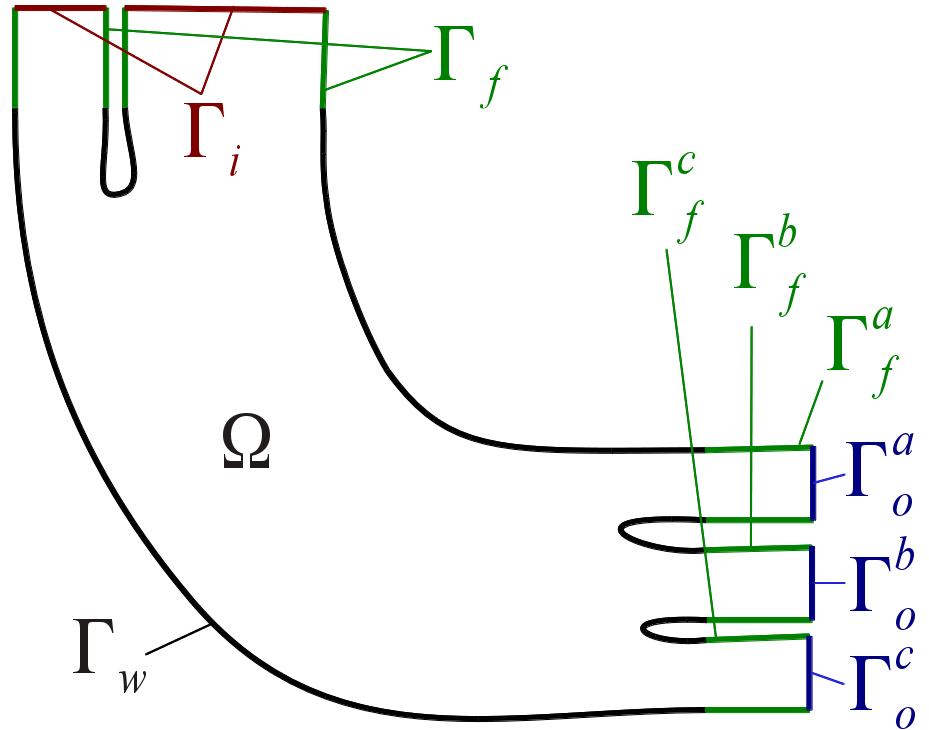
\includegraphics[scale=0.6]{geometrie_skizze_MultOutlet.png}
%\caption{Skizze von $\Om$ mit Bezeichnung der Teile der Oberfläche.}
%\label{Skizze_MultOutlet}
%\end{figure}
\newpage
\subsection{Geometrische Restriktionen}
%
Die Formoptimierung unterliegt zwei geometrischen Restriktionen:
\begin{itemize}
 \item Bauraumrestriktion: Es ist eine optimale Geometrie innerhalb eines fest vorgegebenen Bauraumes gesucht.
\item Übergangsrestriktion: Am Übergang zwischen der zu formoptimierenden Geometrie und der fixen Geometrie soll eine Kante vermieden werden, um Probleme in der Strömungssimulation zu vermeiden.
\end{itemize}
%
\subsubsection{Methode 1: Fixieren am Übergangsbereich}
Formgradient an den Mittelpunkten der Flächen, die an die fixe Geometrie angrenzen gleich 0 setzten.
\begin{figure}[h]
    \centering
    \begin{minipage}[b]{5 cm}
Numerische Berechnung an diesen Stellen ist nicht vertrauenswürdig.\\
Bei bisherigen Berechnungen wurde der Formgradient automatisch auf diesen Flächen gleich null gesetzt.
Dies empfiehlt sich auch für die weiteren Testrechnungen.\\ 
Die Einstellung erfolgt über den Parameter: uer\_fix\_faces\\ (0:nicht fixieren, 1: fixieren).$ $\\
$ $\\
$ $\\
  \end{minipage}
%    \begin{minipage}[b]{1 cm}
%     \end{minipage}
  \begin{minipage}[b]{6 cm}
    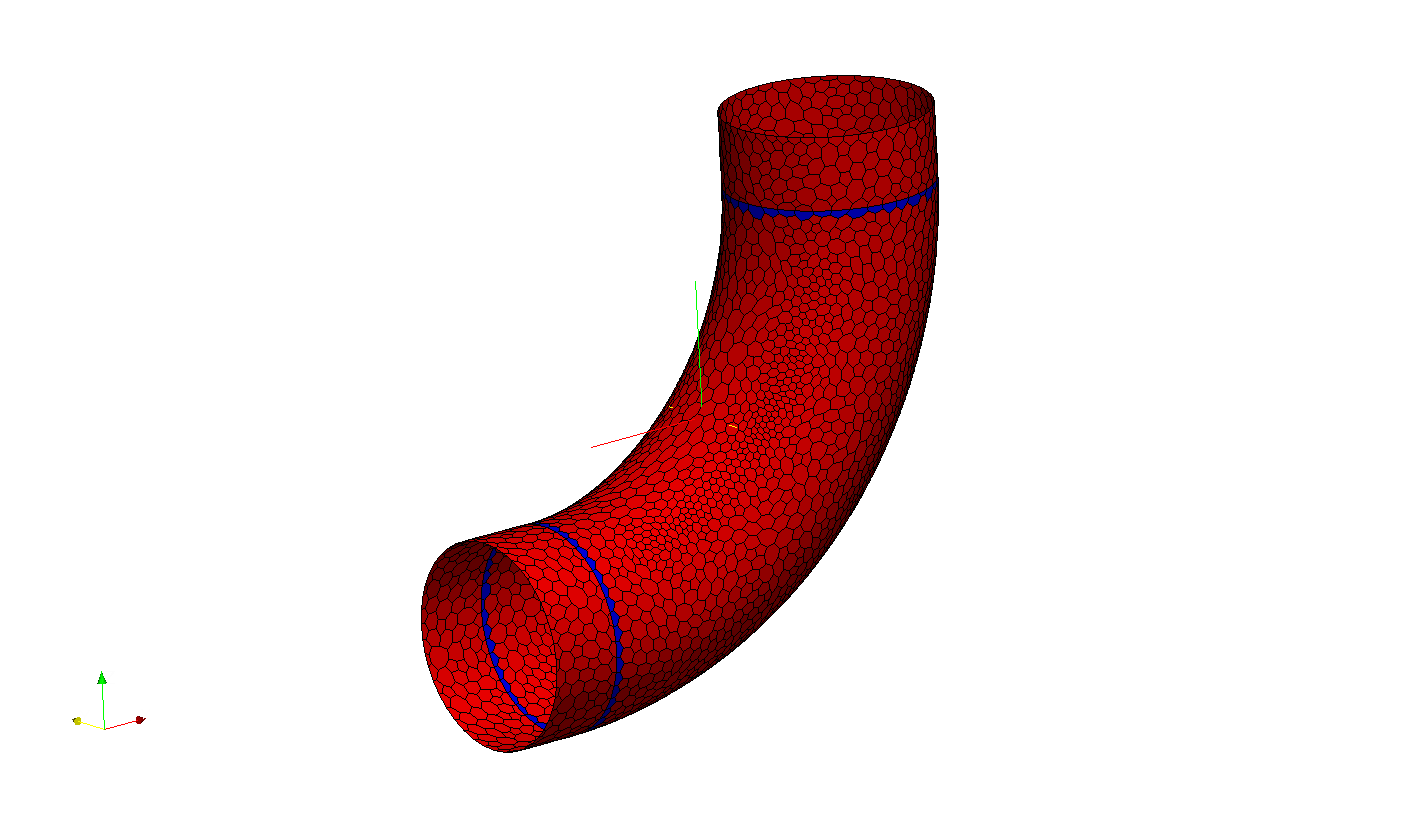
\includegraphics[scale=0.14]{inlet_outlet_fg_fix.png} 
  \caption{BLAU: Faces, auf denen der Formgradient im Flächenmittelpunkt 0 gesetzt wird.}
\label{uer_model}
  \end{minipage}
\end{figure}
\subsubsection{Methode 2: Verwendung von Zielfunktionale für Bauraum und Übergangsrestriktionen}
Um diese Restriktionen in der Formoptimierung zu berücksichtigen, wird das bisher verwendete Zielfunktional $\JJ_{12}$ erweitert zu
\begin{equation}
\nonumber  \JJ_{12}^{\alpha,\varphi}\left( \buu \left( \Om \right) \right)=\JJ_{12}\left( \buu \left( \Om \right) \right)+ \alpha \LL\left(\Om\right) + \varphi \LL_F\left(\Om\right)
 \end{equation}
mit $\LL\left(\Om\right)=\int_\Om \ell\left( x \right)$, $\LL_{F}\left(\Om\right)= \int_{\Om} (d(x,K_F))^2$,
 den Gewichtungsparametern $\alpha \geqslant 0$ (\textbf{bauraum\_gewichtung}), $\varphi \geqslant 0$ (\textbf{fix\_gewichtung}) und der Distanzfunktion  
$d\left(x,K_F\right)= c_1 \underset{y\in K_F}{min}\left|x-y\right|$.
Im Falle der Barriere-Methode ist 
%\begin{equation}
$\ell\left( x \right)= \left|\mbox{ln} \; d\left(x,K^c\right)\right| $ 
%\end{equation}
und im Falle des Penalty-Verfahrens ist 
%\begin{equation}
%\ell\left(\Om\right)= \left(1-\chi_K\left(x\right)\right) \left(d\left(x,K\right)\right)^{\beta}.
$\ell\left( x \right)= c_2\left(d\left(x,K\right)\right)^{\beta}$, 
%\end{equation}
mit $\beta>0$ (\textbf{bauraum\_straf\_potenz}).
Die Skalierungsfaktoren $c_1, c_2$ werden im Abschnitt \ref{skalierung_bauraum} behandelt.
Die Geometrie $K$ bezeichnet die Bauraumgeometrie, $K^c=\mathbb{R}^n \setminus K$ und die Geometrie $K_F$ bezeichnet den zulässigen Bereich der Geometrie im Übergang zwischen den fixen und den zu formoptimierenden Teilen. % (siehe Abbildung \ref{strahlfl0}).  
Der Parameter \textbf{bauraum\_restriktion} gibt an ob bzw. welche Methode im Umgang mit der Bauraumrestriktion verwendet werden soll.
Will man die Bauraumgewichtung $\alpha$ während der Formoptimierung erhöhen (im Falle des Penalty-Verfahrens) bzw. verringern (im Falle der Barriere-Methode) so können die Parameter 
\textbf{OuterLoopCycleNr} (Tabelle \ref{tab:abbruch}) und \textbf{bauraum\_modification\_scale} verwendet werden. 
%An jeder dieser Erzeugenden kann eine Restriktionskurve aufgetragen werden (siehe Abbildung \ref{strahlfl0}). 
%Diese setzt sich aus einem linearen Anteil und einem Term höherer Ordnung zusammen. 
%
%
%Der Benutzer kann die Restriktionsgeometrie über die Parameter: \textbf{uer\_pow} (Grad der Potenzfunktion des nichtlinearen Anteils), \textbf{uer\_nonlinear}, \textbf{uer\_linear} (siehe Abb. \ref{uer_model}) steuern.
%Der Parameter \tuer\_pow gibt den Grad der Potenzfunktion des nichtlinearen Anteils an. 
%Zur Bedeutung der anderen Parameter siehe Skizze \ref{uer_model}.
%Möchte man z.B. einen glatten Übergang ohne Kante, so ist uer\_linear = 0 zu setzten. 
%Je größer uer\_linear bzw. uer\_nonlinear desto steiler ist der Kurvenverlauf.
\begin{figure}[h]
    \centering
    \begin{minipage}[b]{5 cm}
Innerhalb des Bereiches, welcher durch den Abstand zur fixen Geometrie (\textbf{uer\_bereich}) festgelegt ist, erfolgt die Übergangsrestriktion.
Der Benutzer kann die Restriktionsgeometrie mit den Parametern: \textbf{uer\_pow} (Grad der Potenzfunktion des nichtlinearen Anteils), \textbf{uer\_nonlinear} und \textbf{uer\_linear} (siehe Abb. \ref{uer_model}) steuern.\\
$ $\\
  \end{minipage}
    \begin{minipage}[b]{0.5 cm}
$ $\\
     \end{minipage}
  \begin{minipage}[b]{6 cm}
    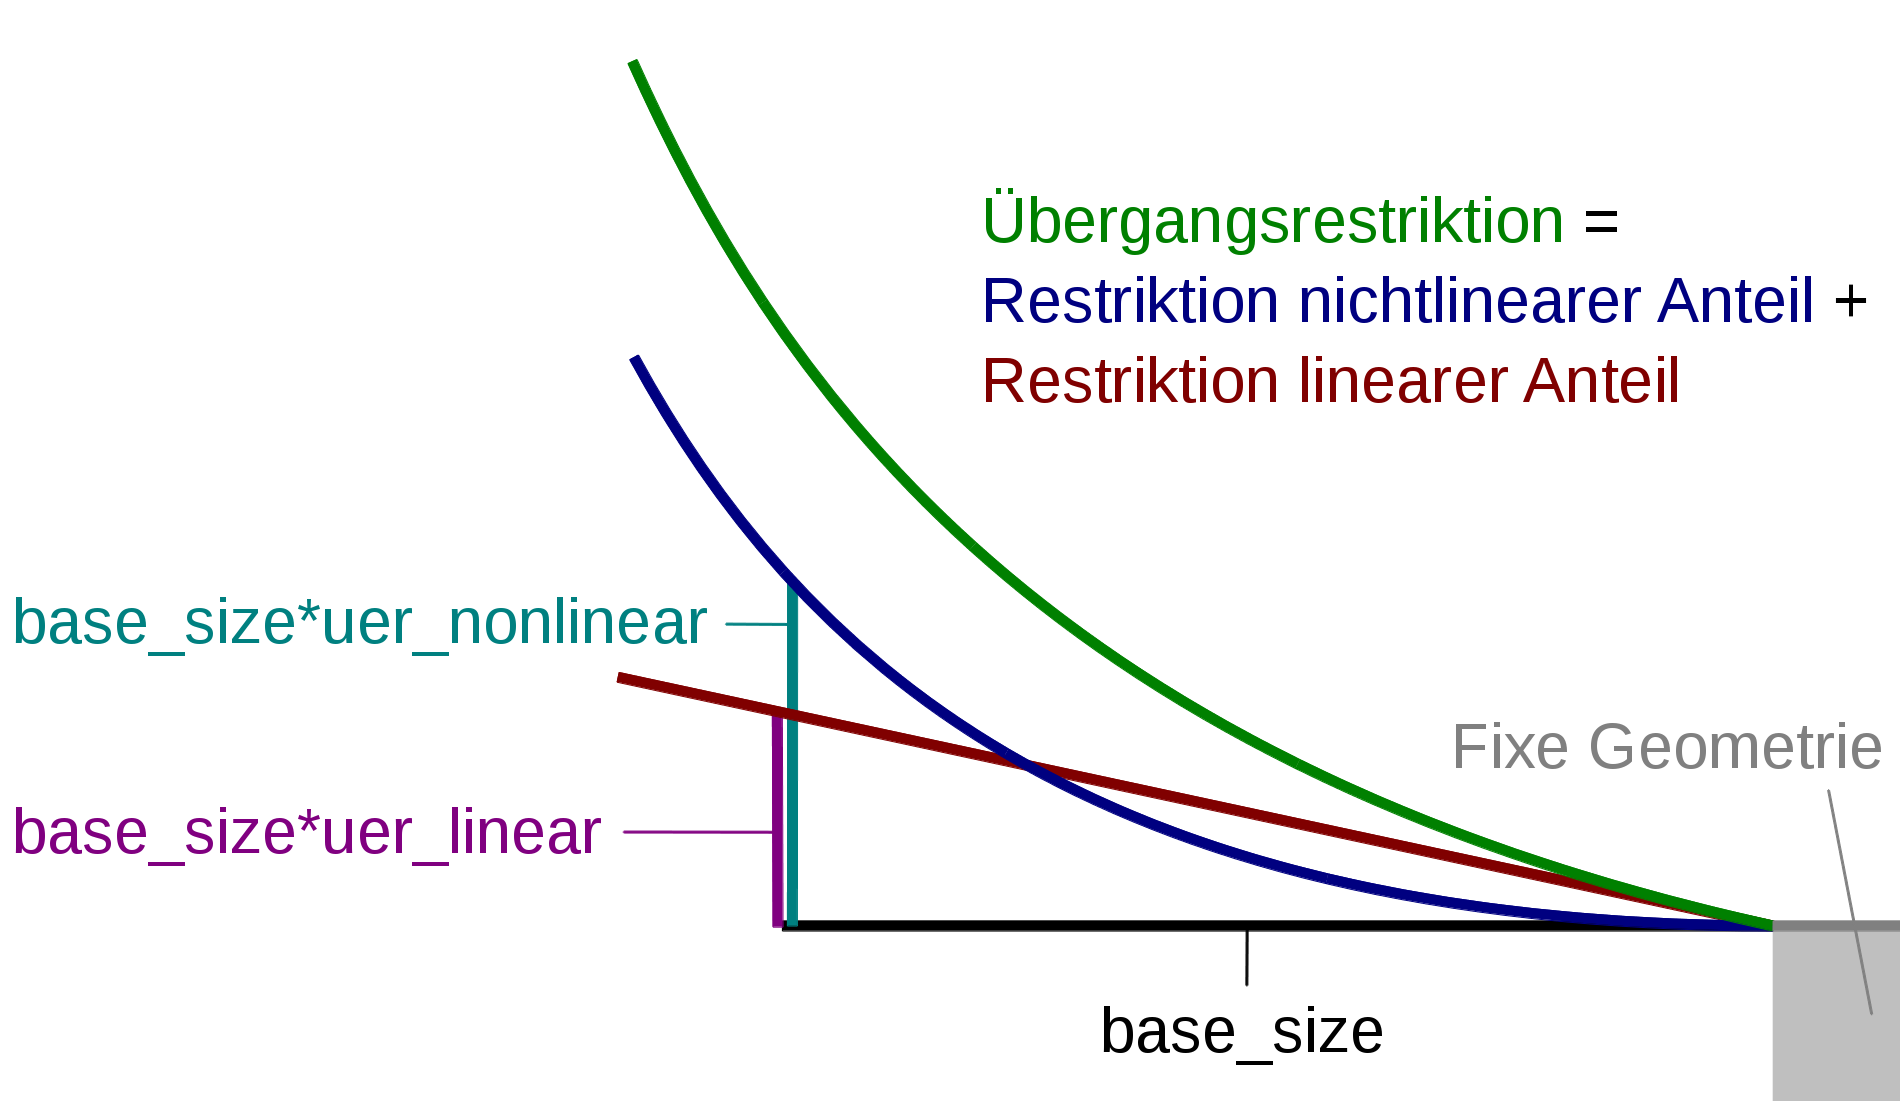
\includegraphics[scale=0.4]{uer_funk2.png}
  \caption{Übergangsgeometrie.} 
\label{uer_model}
  \end{minipage}
\end{figure}
%
\begin{figure}[htbp]
  \centering
%    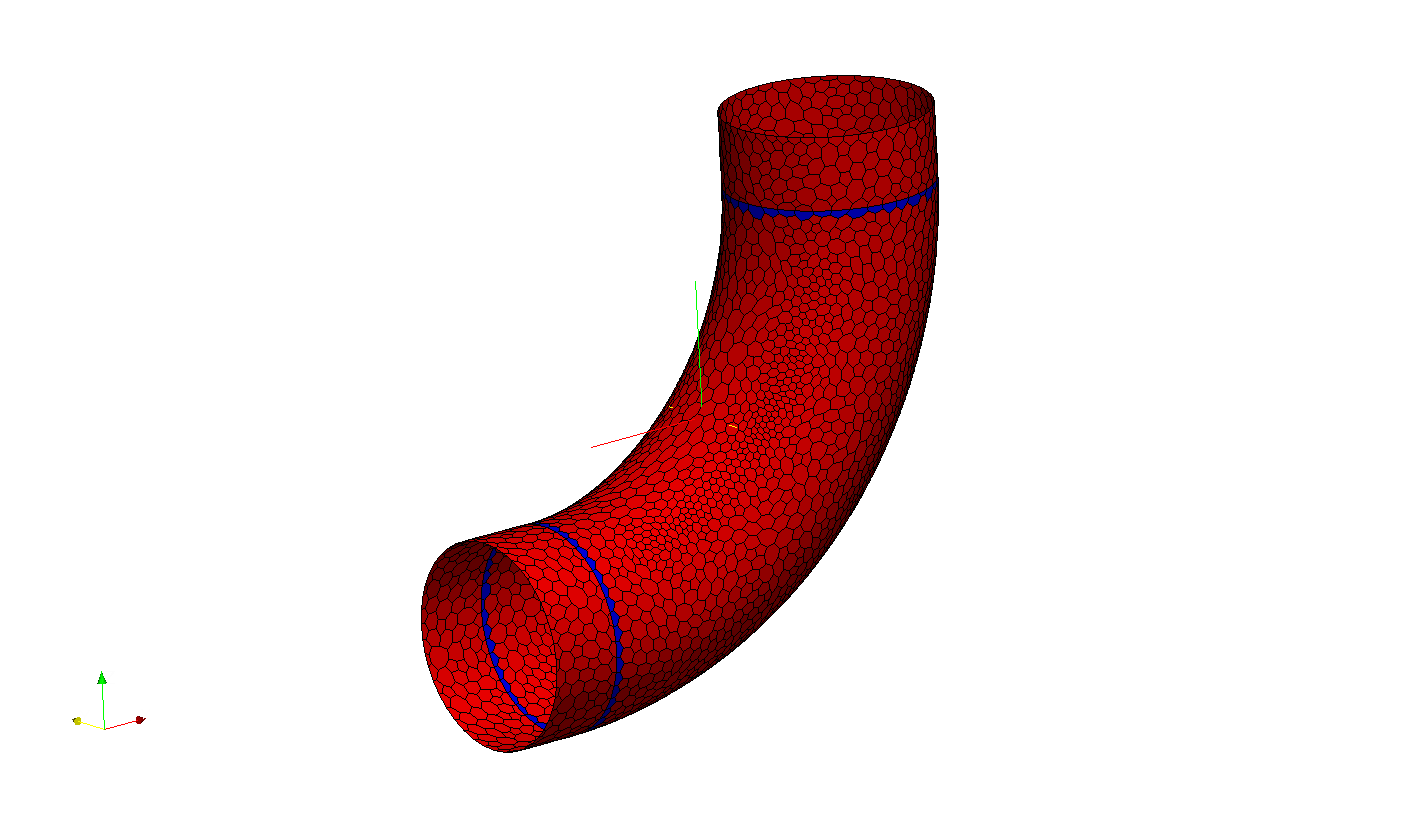
\includegraphics[scale=0.13]{inlet_outlet_fg_fix.png} 
    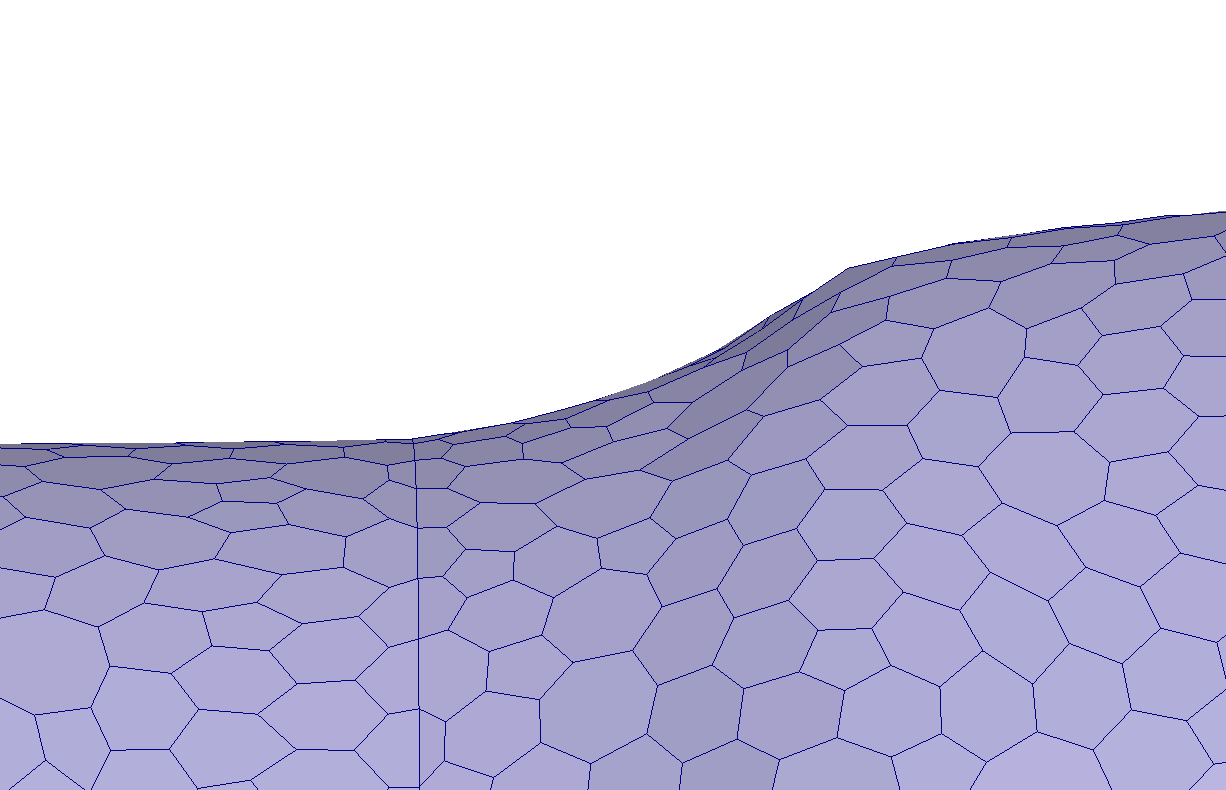
\includegraphics[scale=0.1]{restriktion1.png} 
    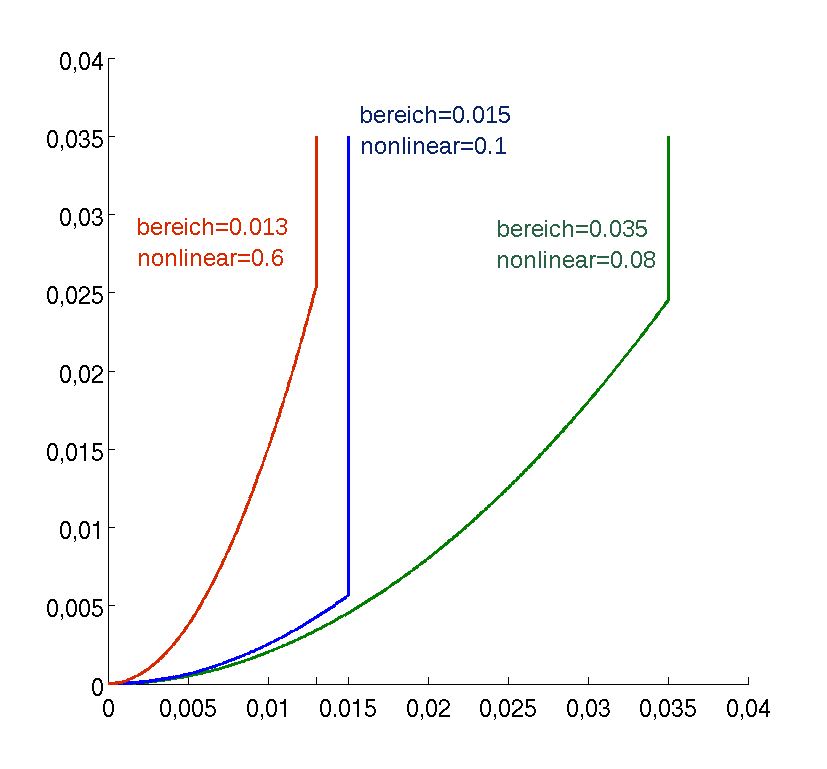
\includegraphics[scale=0.25]{uer_bereich_nonlinear.png} 
%    \includegraphics[scale=0.1]{Rohr1a_J0_v2.png} 
  \caption{ Links: Geometrie am Übergang. Rechts: unterschiedliche Übergangsrestriktionen.} 
\label{uer_3kurven}
\end{figure}
$ $\\
In Abbildung \ref{uer_3kurven} sind Übergangskurven bei drei unterschiedlichen Parametereinstellungen dargestellt. Um starke Krümmungen der Geometrie zu verhindern, ist die Variante in grüner Farbe zu empfehlen.
%
\subsubsection{Heuristische Skalierung der Zielfunktionale bei geom. Restriktionen}
\label{skalierung_bauraum}
%
Um gleiche Größenordnungen von geometrischen Zielfunktionalen und physikalischen Zielfunktionalen zu erzielen, 
verwenden wir eine Skalierung $c_1$ der Raumkoordinaten und eine Skalierung $c_2$ der Funktion $\ell(d)$ unter Verwendung der Startgeometrie $\Om^0$.
Im Falle des \textbf{Penalty-Verfahrens} werden die Parameter $c_1$ und $c_2$ so gewählt, dass die Gleichungen 
\begin{eqnarray}
\int_{\Sigma\left(d_{min}\right)}\int_0^{c_1 d_{max}} c_2 d^{\beta} \text{d}d &=& \JJ_{12}\left( \buu \left( \Om^0 \right) \right), \\
c_2\left(c_1 d_{max}\right)^\beta &=& \lVert \DD \JJ_{12}^\alpha \left( \Om^{0}  \right) \rVert_{L^\infty \left(\Gamma_w^0\right)}
\end{eqnarray}
erfüllt sind, wobei $d_{min}$ und $d_{max}$ anzugeben sind durch die Wahl der Parameter \textbf{dminDS} und \textbf{dmaxDS} für die Bauraumrestriktion (bzw. analog \textbf{dminIF} und \textbf{dmaxIF} für die Übergangsrestriktion).\\
%
\begin{figure}[htbp]
  \centering
    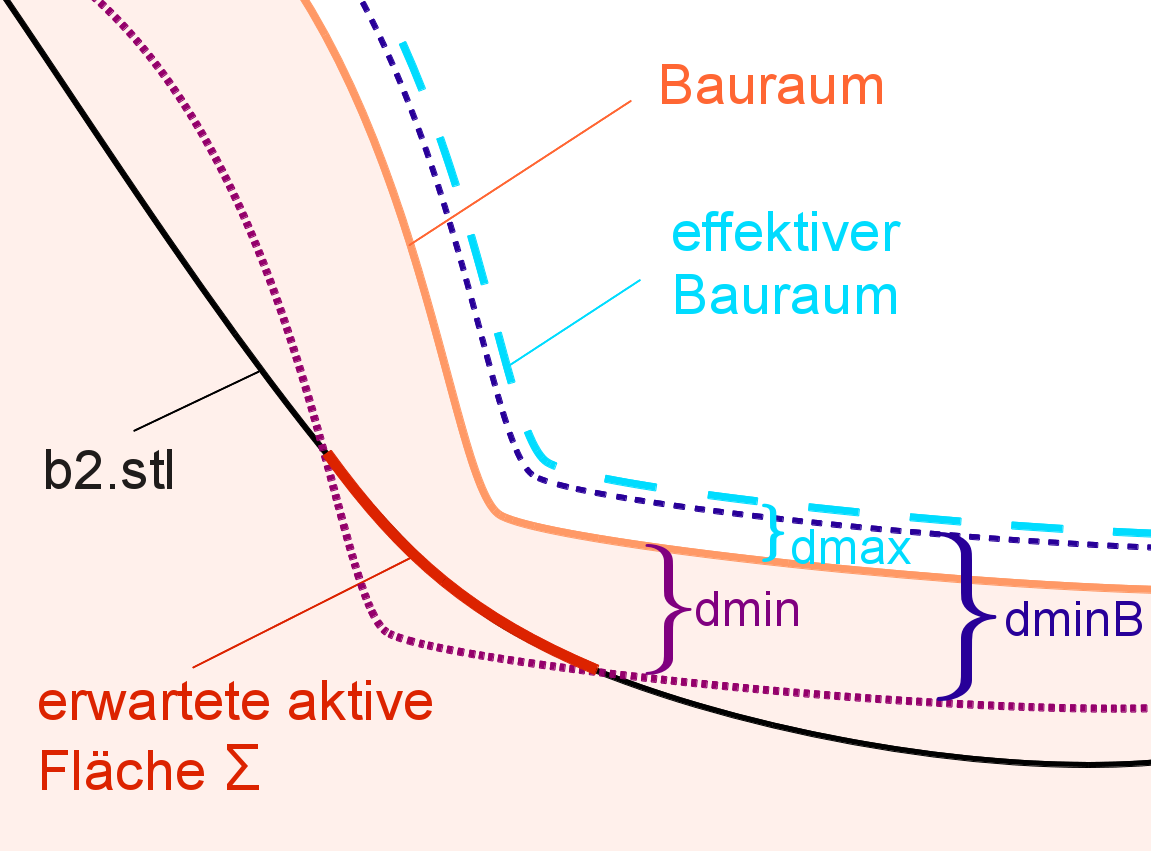
\includegraphics[scale=0.45]{bauraum_parameter1deutsch.png} \quad
    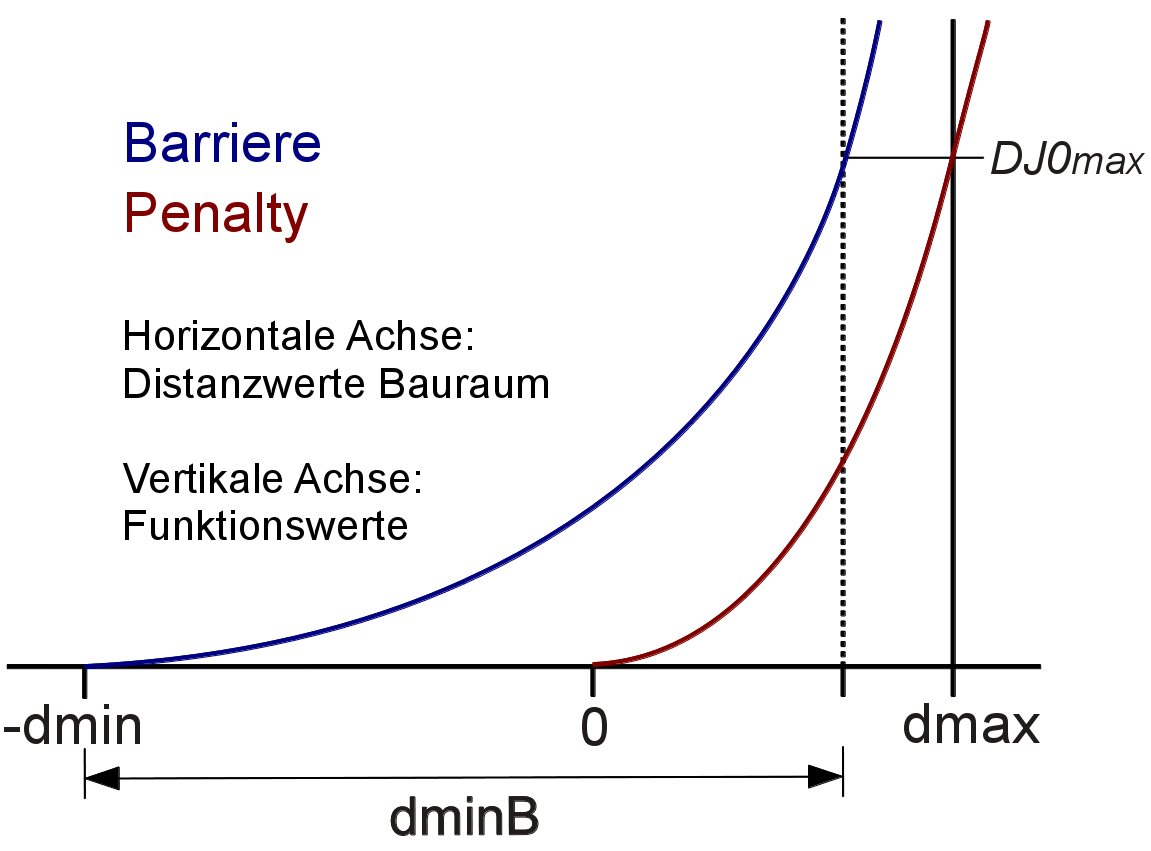
\includegraphics[scale=0.45]{bauraum_parameter2.png} 
  \caption{Links: Skizze Bauraum. Rechts: Funktionen: Penalty, Barriere.} 
\label{fig:bauraum_parameter}
\end{figure}
%
$ $\\
Im Falle der \textbf{Barriere-Methode} kann anstelle des geometrischen Bauraumes (\emph{bds.stl}) ein effektiver Bauraum gewählt werden.
Hierbei wird der Bauraum um die Länge \textbf{dmaxDS} (Einheit in Meter) vergrößert. 
Wird dieser Paramteter gleich 0 gesetzt, so ist der effektive Bauraum gleich dem geometrischen Bauraum.
Die Einstellung von \textbf{dmaxDS} größer 0 ist insbesondere für jene Fälle angedacht, bei denen die Startgeometrie außerhalb des geometrischen Bauraumes liegt.% (Abbildung \ref{fig:paraviewBauraum}).
Die Skalierungsgrößen $c_1$ und $c_2$ werden so gewählt, dass die Gleichungen 
\begin{eqnarray}
\int_{\Sigma\left(d_{min}\right)}\int_0^{c_1 d_{minB}} c_2 d^{\beta} \text{d}d &=& \JJ_{12}\left( \buu \left( \Om^0 \right) \right), \\
c_2\left(c_1 d_{minB}\right)^\beta &=& \lVert \DD \JJ_{12}^\alpha \left( \Om^{0}  \right) \rVert_{L^\infty \left(\Gamma_w^0\right)}
\end{eqnarray}
erfüllt sind, wobei $d_{min}$ und $d_{minB}$ durch die Wahl der Parameter \textbf{dminDS} und \textbf{dminBDS} anzugeben sind (siehe Abbildung \ref{fig:bauraum_parameter}).
%
\subsubsection{Methode 3: Dämpfung im Übergangsbereich}
Dämpfung des Formgradienten im Übergangsbereich.
%\item Lösen der Laplace-Beltrami Gleichung mit Randbedingungen gleich 0 an der Übergangskurve.  
%\begin{columns}[c]
%\column[c]{6cm}
\begin{figure}[htbp]
  \centering
%    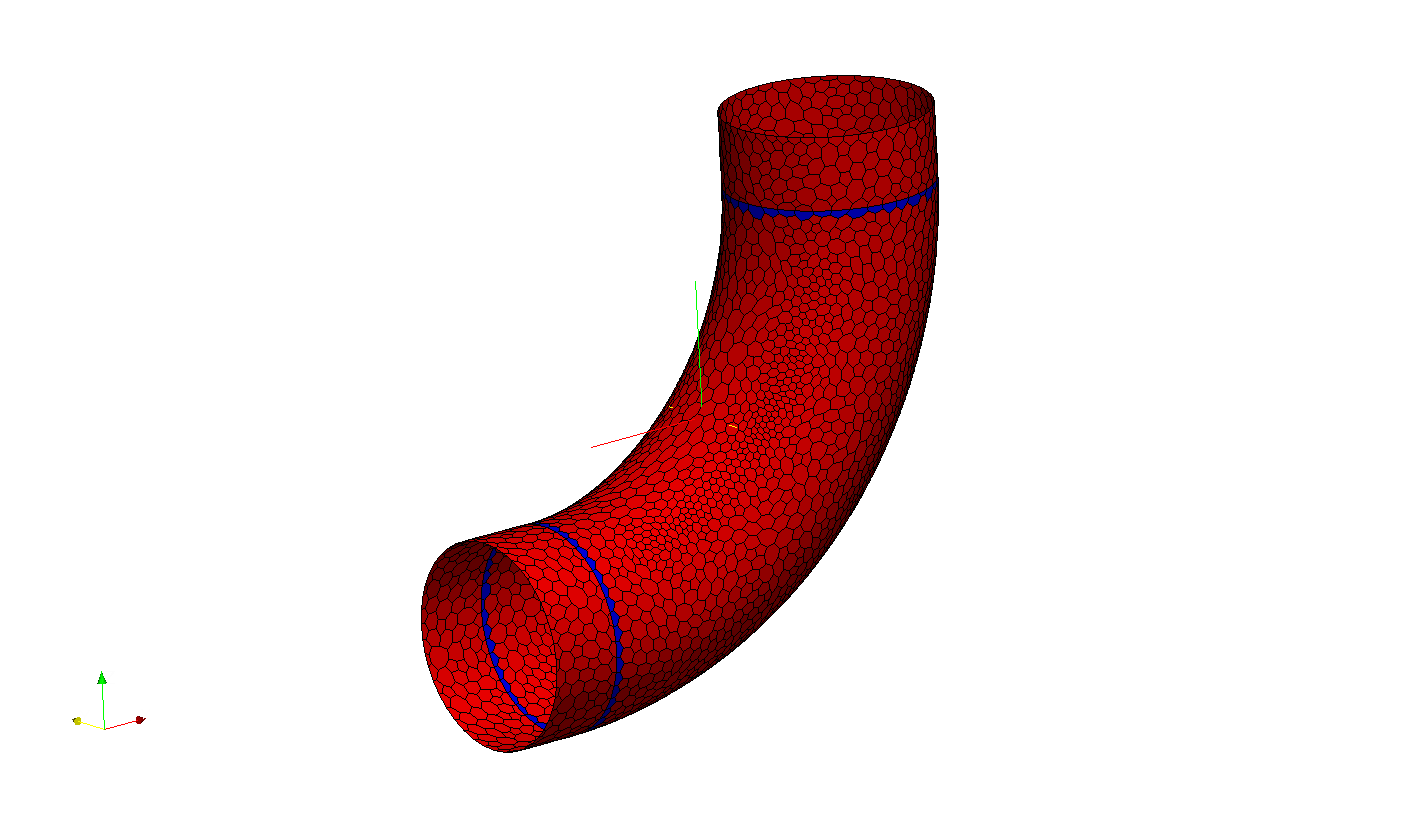
\includegraphics[scale=0.13]{inlet_outlet_fg_fix.png} 
    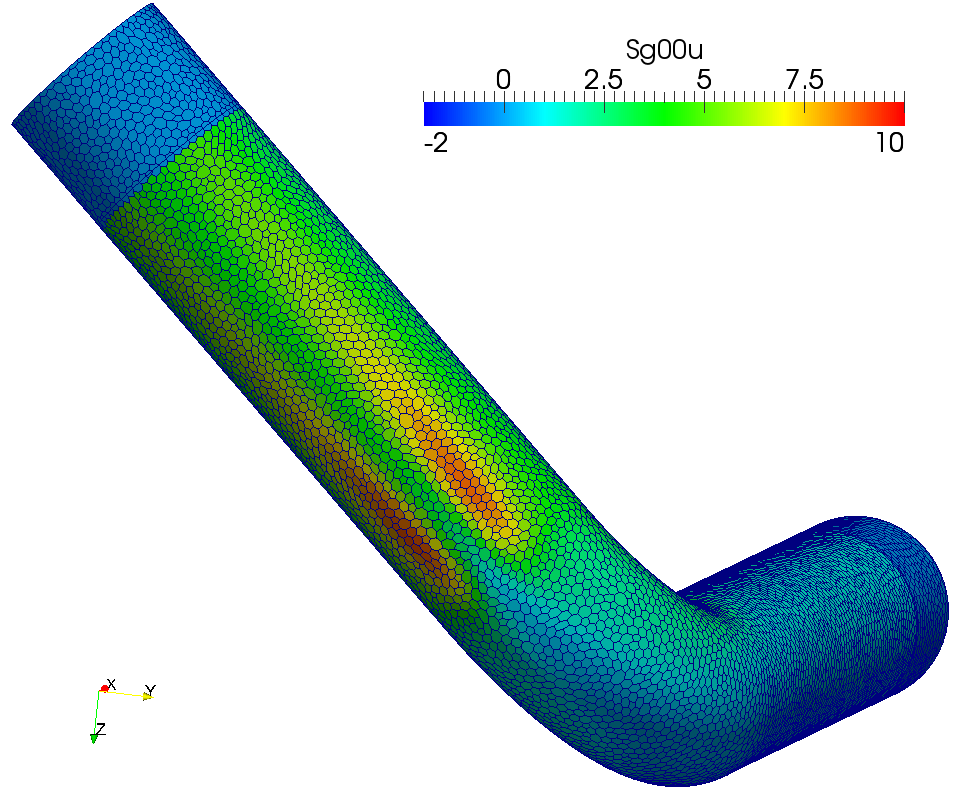
\includegraphics[scale=0.16]{Rohr3_damp0.png} 
    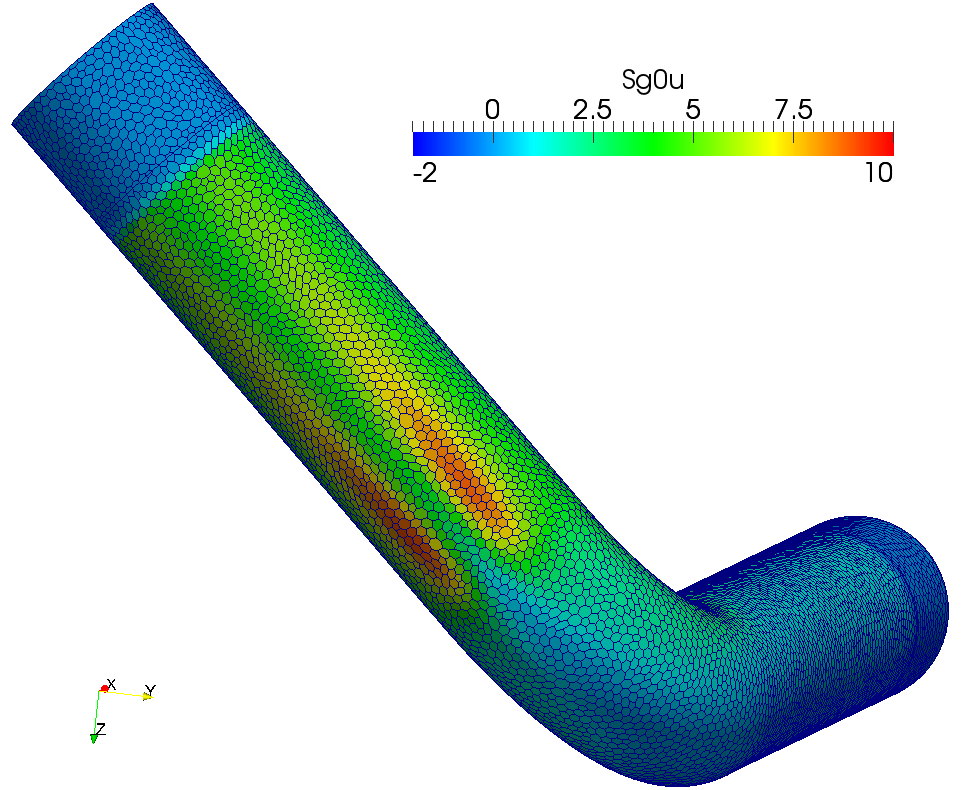
\includegraphics[scale=0.16]{Rohr3_damp1.png} 
  \caption{ Links: Rohr 3 ohne Dämpfung. Rechts: Rohr 3 mit Dämpfung.} 
\end{figure}
%\column[c]{5cm}
$ $\\
Eigenschaften:
\begin{itemize}
\item - Ungünstig bei unzulässiger Startgeometrie.
\item - Unerwünschte Effekte im Übergang von gedämpftem zum ungedämpften Bereich.
\item + Einfache Benutzerhandhabung, da kein zusätzlicher Parameter erforderlich ist.
\end{itemize}
%\end{columns}
%
\begin{figure}[htbp]
  \centering
%    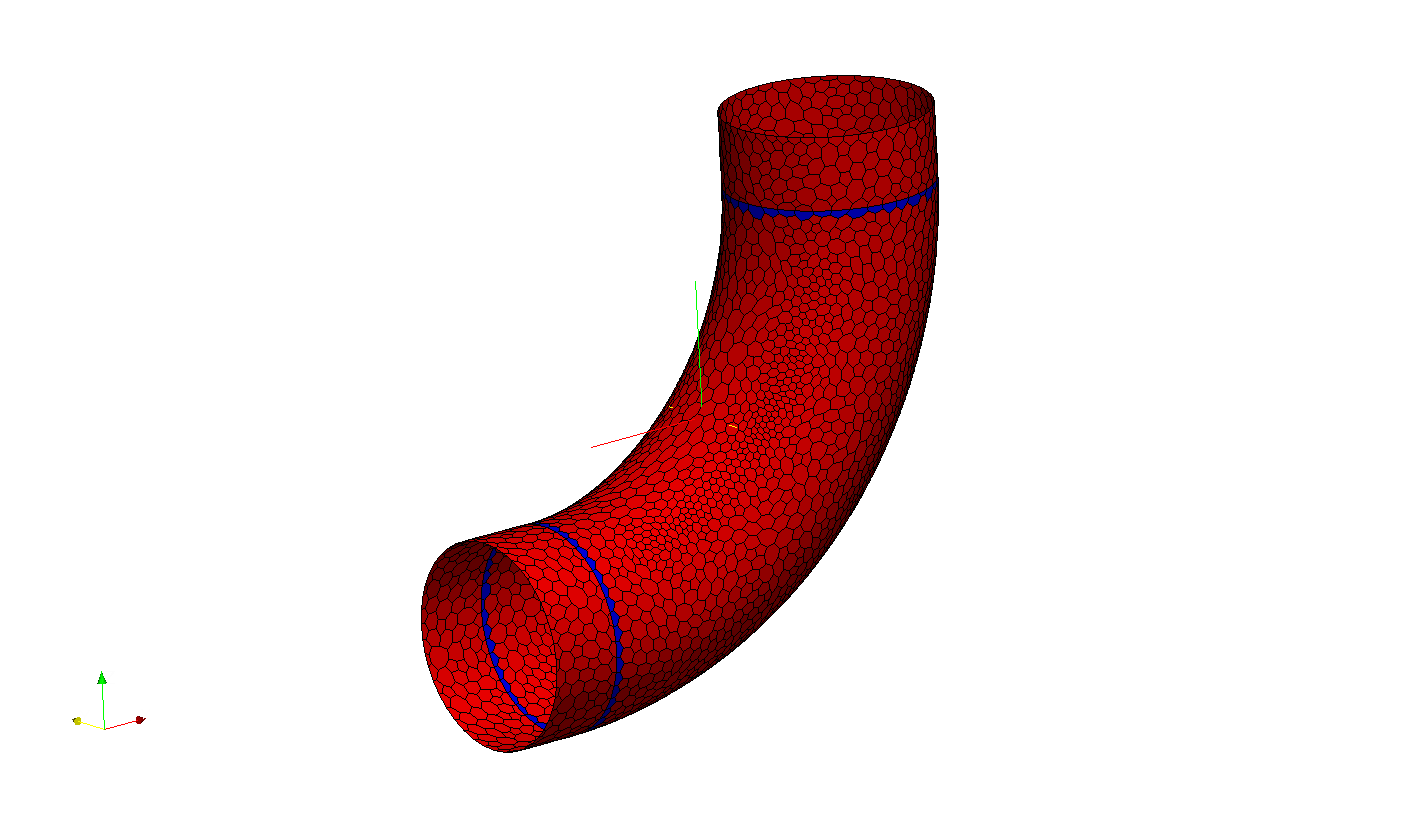
\includegraphics[scale=0.13]{inlet_outlet_fg_fix.png} 
 %   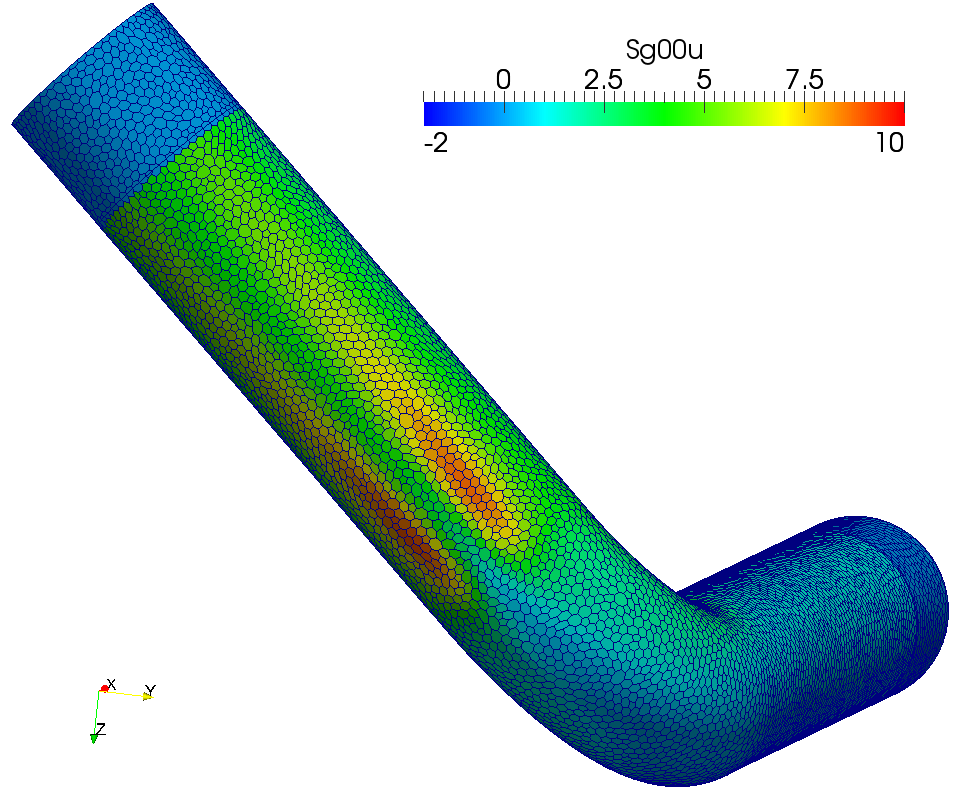
\includegraphics[scale=0.1]{Rohr3_damp0.png} 
%    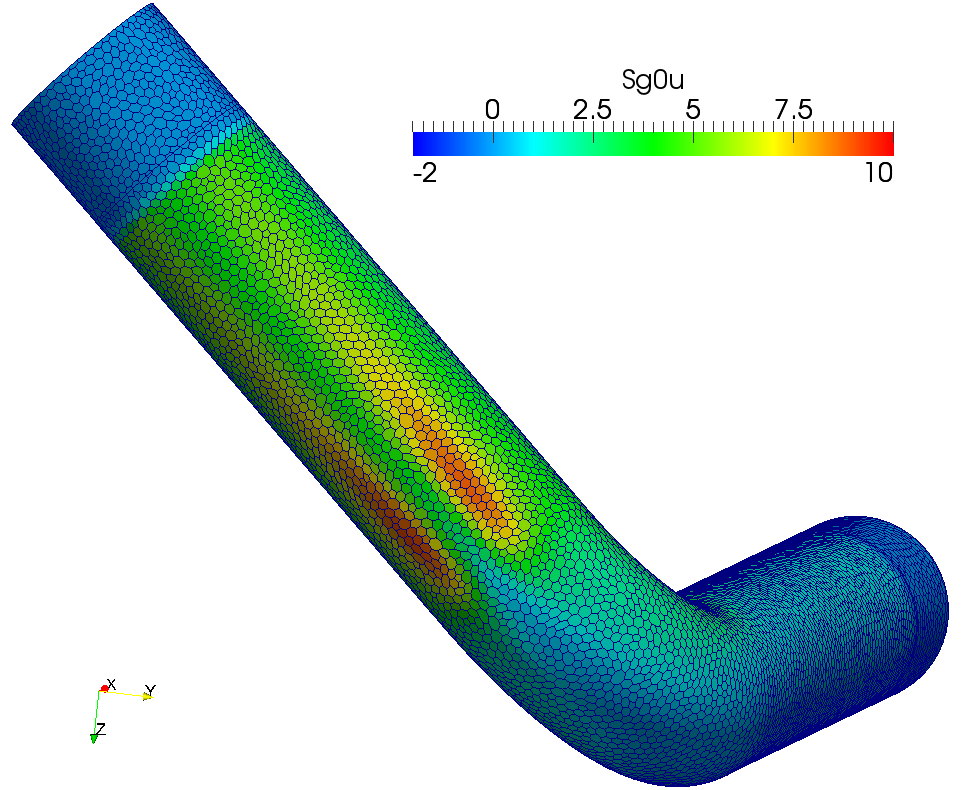
\includegraphics[scale=0.1]{Rohr3_damp1.png}\\
     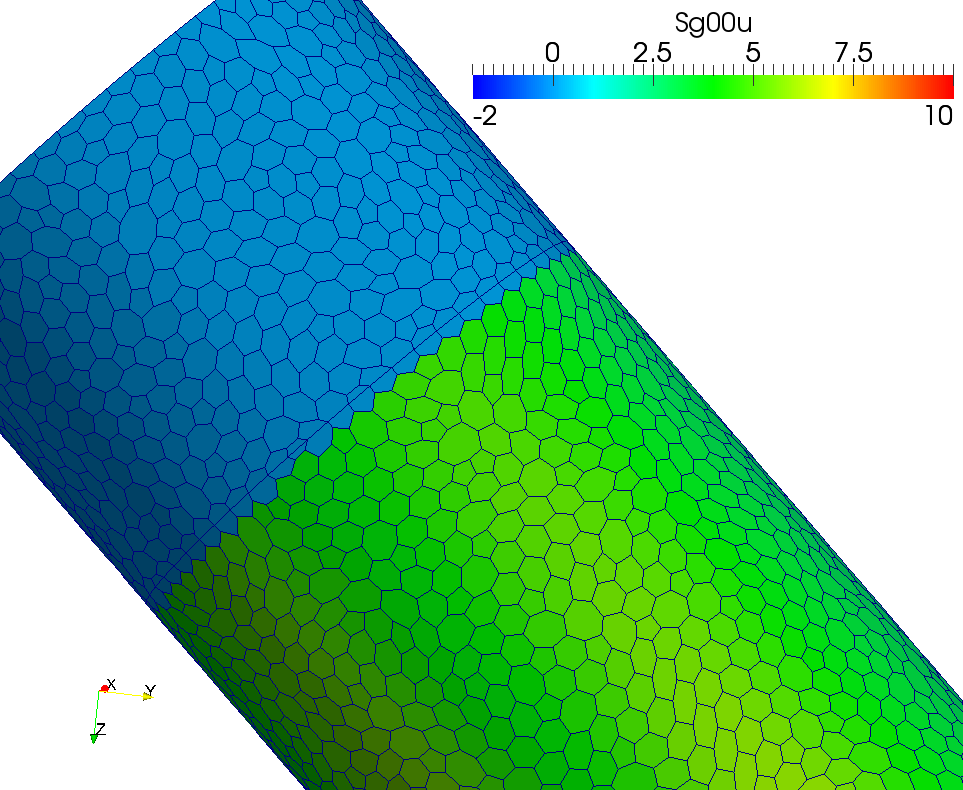
\includegraphics[scale=0.085]{Rohr3_damp_0b.png} $ $
     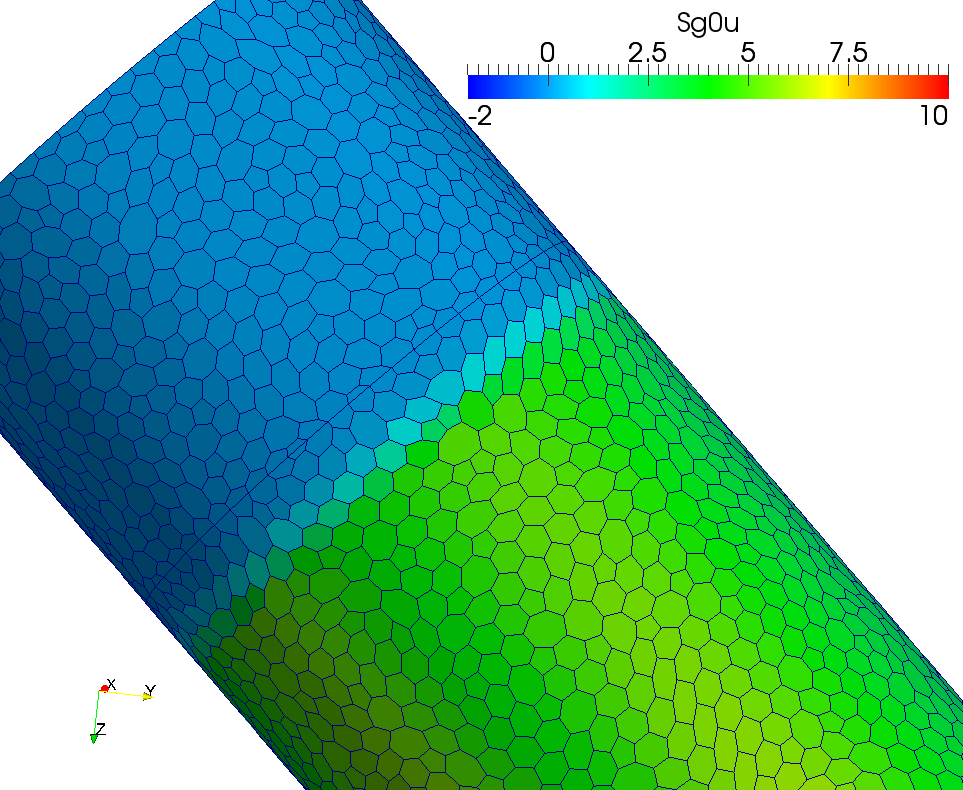
\includegraphics[scale=0.085]{Rohr3_damp_0a.png} $ $
     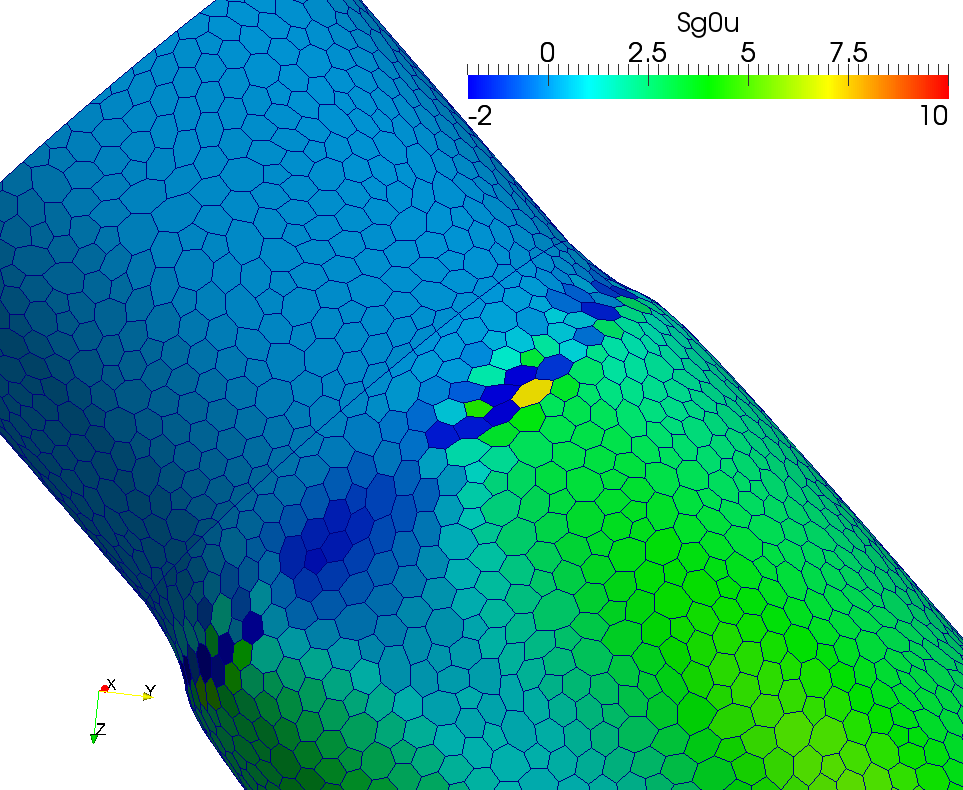
\includegraphics[scale=0.085]{Rohr3_damp40.png}
%    \includegraphics[scale=0.1]{Rohr1a_J0_v2.png} 
\caption{Detailansicht: links: ohne Dämpfung, mitte: mit Dämpfung, 
rechts: gedämpfter Forgradient nach 40 Iterationen.}
\end{figure}
\subsubsection{Methode 4: Glättung des Formgradienten}
%
Lösen der Laplace-Beltrami Gleichung mit Randbedingungen gleich 0 auf der Übergangskurve.  
\begin{figure}[htbp]
  \centering
    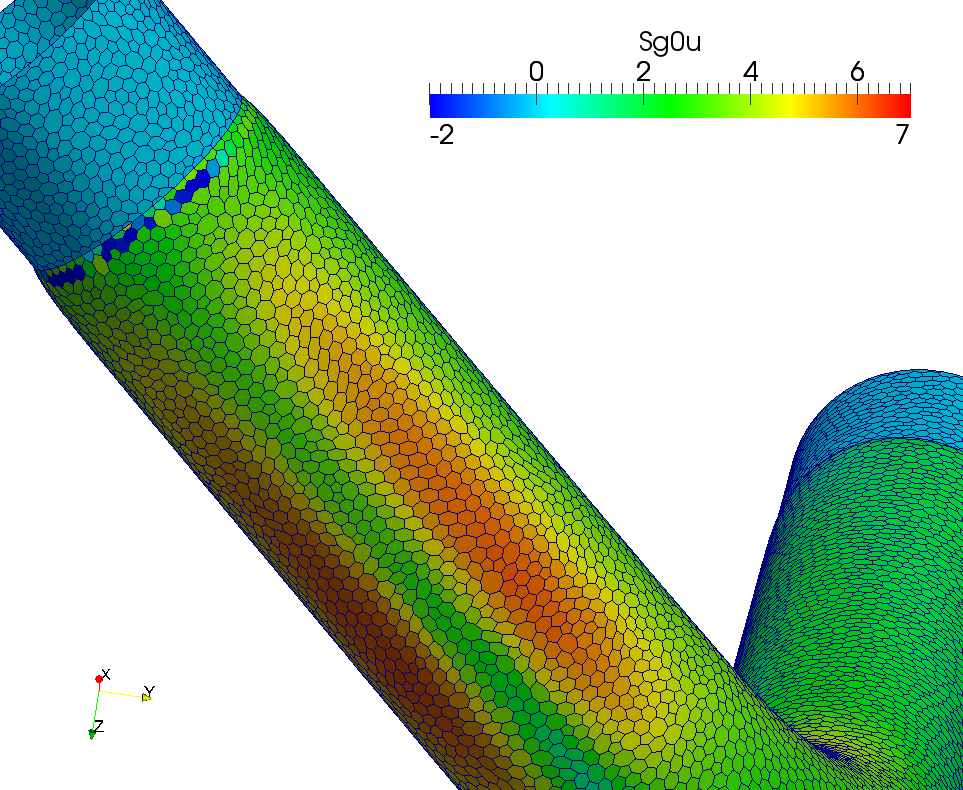
\includegraphics[scale=0.12]{Rohr3_lb0.png} 
    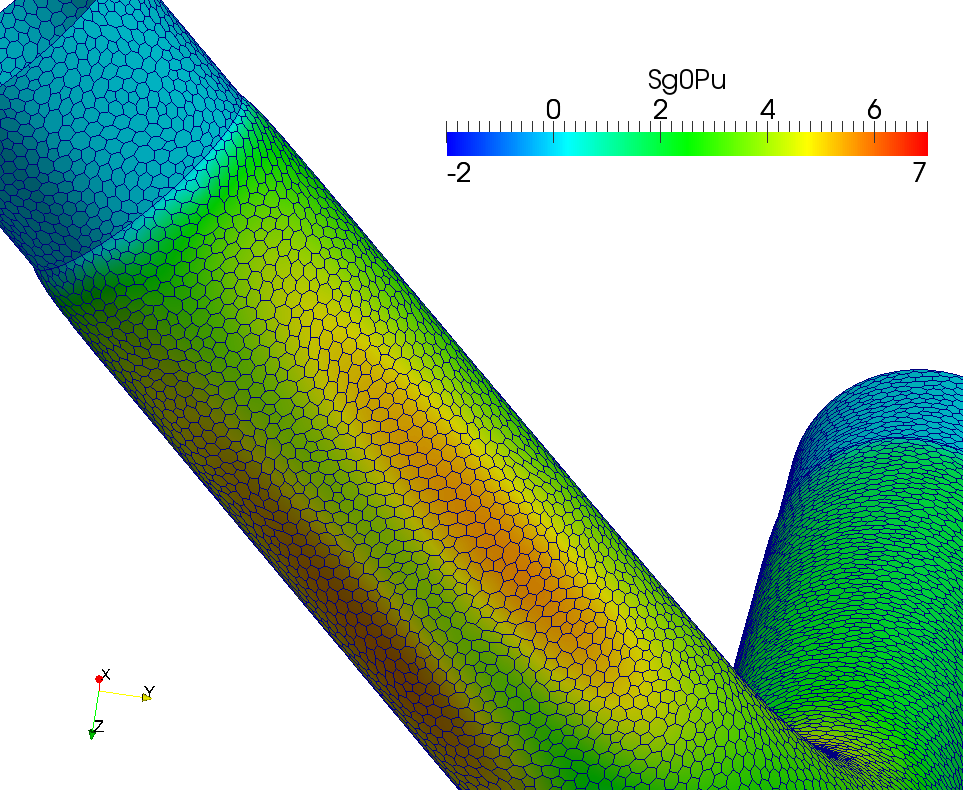
\includegraphics[scale=0.12]{Rohr3_lb1.png} 
  \caption{Rohr 3: links: ohne LB-Glättung, rechts: mit LB-Glättung.} 
\end{figure}
$ $\\
\begin{eqnarray}
\label{LB1} -\varepsilon \Delta_\Gamma w + w &=& -g_{\JJ_{12}}  \qquad \mbox{auf}\quad \Gamma\\
w &=& 0 \qquad \qquad \, \mbox{auf}\quad \partial \Gamma
\end{eqnarray}
$ $\\
Der Parameter $\varepsilon$ in Gleichung \eqref{LB1} entspricht dem Parameter \textbf{scaleLB} in Tabelle \ref{tab:parameter8}.
Falls keine Laplace-Beltrami Glättung erfolgen soll, so ist dieser Parameter auf 0 zu setzen. Erfahrungsgemäß sollte der Parameter im Bereich [1e-6, 1e-3] gewählt werden.
Die Glättung wird stärker je größer der Paramter gewählt wird. 
%
\begin{table}[h]
\centering
\begin{tabular}{|p{3.1cm}|p{1cm}|p{1.2cm}|p{0.7cm}|p{0.7cm}|p{5.7cm}|} %lcrp
\hline
\cellcolor{light-gray} Parametername & \cellcolor{light-gray} Default-wert & \cellcolor{light-gray} Zuläs-sigkeit & \cellcolor{light-gray} RLR & \cellcolor{light-gray} M23 & \cellcolor{light-gray} Beschreibung\\
\hline
uer\_bereich                   &  0.01  &  [0,100]   & 0.015 & 0.35 & Übergangsrestriktion: Bereich in m.\\
\hline
uer\_nonlinear                 &  0.2   &  [0,100]   & 0.6   & 0.3 & Übergang.: <<1: flache, >>1:steile Kurve.\\
\hline
uer\_linear                    &   0    &  [0,100]   & 0     & 10 & Übergang.: <<1: flache, >>1:steile Gerade.\\
\hline
uer\_pow                       &  2     &  [0,10]    & 2     & 2 & Übergang: Potenz d. Übergangsfkt.\\
\hline
bauraum\_restriktion           &  1     &  \{0,1,2\} &  2    & 0 & 0:ohne Bauraum, 1:Barriere, 2:Penalty.\\
\hline
%bauraum\_gewichtung            &  1     &  [0,1e22]  &  1    & 1 & Gewichtung $\alpha$ für Bauraumrestriktion.\\
%\hline
bauraum\_straf\_potenz        &  2     &  [1,3]     &  2    & 2 & Potenz $\beta$ bei Penalty-Verfahren.\\
\hline
fix\_gewichtung                &  1     &  [0,100]   &  1    & 1 & Gewichtung $\varphi$ für Übergangsrestr.\\
\hline
uer\_fix\_faces                &  1     &  \{0,1\}    & 1     & 1 & Übergangsrestriktion: Methode 1 verwenden: 0:nein, 1:ja.\\
\hline
scaleShapeGradientFix          &  1     &  \{0,1\}    & 1     & 0 & Übergangsrestriktion: Methode 3 verwenden: 0:nein, 1:ja.\\
\hline
scaleLB                        &  1e-5  &  [0,1]      & 5e-5  & 1e-3 & Übergangsrestriktion: Methode 4 Glättungsparameter: 0 keine Glättung, 1 starke Glättung.\\
\hline
\end{tabular}
\caption{Geometrische Restriktionen 1.}\label{tab:parameter8}
$ $\\
%\end{table}
%
%\begin{table}[h]
%\centering
\begin{tabular}{|p{2.5cm}|p{3.7cm}|p{1cm}|p{4.1cm}|} %lcrp
\hline
\cellcolor{light-gray} Parametername & \cellcolor{light-gray} Defaultwert & \cellcolor{light-gray} Zuläs-sigkeit  & \cellcolor{light-gray} Beschreibung\\
\hline
dminIF, dmaxIF   &  1e-2, 5e-3  &  [0,10]       & Übergangsrestr.: Skalierung.\\
\hline
dminDS, dminDS   &  1e-2, 5e-3  &  [0,10]      & Bauraumrestr.: Skalierung.\\
\hline
dminBDS          &  (dminDS+dmaxDS)*0.8  &  [0,10]      & Bauraumrestr.: Skalierung.\\
\hline
\end{tabular}
\caption{Geometrische Restriktionen 2 (Detail).}\label{tab:parameter8}
%\end{table}
%
$ $\\
%\begin{table}[h]
%\centering
\begin{tabular}{|p{1.6cm}|p{1.2cm}|p{1cm}|p{7.6cm}|} %lcrp
\hline
\cellcolor{light-gray} Parameter- name & \cellcolor{light-gray} Default-wert & \cellcolor{light-gray} Zuläs-sigkeit  & \cellcolor{light-gray} Beschreibung\\
\hline
restart\_opt      &  0  &  \{0,1\}       & Ausgangsgeometrie wall0.stl für Geometrieänderung verwenden: 0:nein, 1:ja.\\
\hline
damp           &  3(0 0 0)  &  [0,1e20]      & Dämpfungsparameter ($\rho_2$, $\rho_1$, $\rho_{1a}$, $\rho_{1b}$, $\rho_{1c}$), optional anzugeben anhand der Einträge in Testlauf\_Info.txt.\\
\hline
\end{tabular}
\caption{Optionale Restart - Parameter.}\label{tab:parameter9}
\end{table}
%
\newpage 
$ $\\
\newpage
\subsection{Topologieoptimierung}
%
Falls die Topologieoptimierung durchgeführt werden soll ist er Parameter \textbf{topOpt} auf 1 zu setzen.
Die angepasste Impulsgleichung der Strömung in einem porösen Medium lautet:
%The adapted momentum equation for a porous medium:
\begin{equation}
 \nabla \cdot \left(\buu \buu^{T} \right) -\nu \Delta \buu + \nabla p \, \, \textcolor{blue}{ + \, P_V \buu + P_I \left| \buu \right| \buu } = \bzz,
\end{equation}
Die maximalwerte für $P_V$ und $P_I$ sind durch die Parameter \textbf{porosityV} und \textbf{porosityI} anzugeben.
Diese Werte werden mit dem Parameter \textbf{startPOR} multipliziert um die Startporosität festzulegen.\\
$ $\\
%
\begin{minipage}[b]{9.2 cm}
Es scheint numerisch notwendig, Grenzwerte $\TT_{upper}$ (\textbf{thresholdTOPupper}) und $\TT_{lower}$ (\textbf{thresholdTOPlower}) festzulegen, bei denen die Porosität erhöht bzw. verringert wird. 
Theoretische Festsetzung wäre  $\TT_{upper}=\TT_{lower}=0$.\\
Separates Skalieren der Werte größer als $\TT_{upper}$ und jener kleiner $\TT_{lower}$ führt zu $\overline{\alpha}$ (siehe rechte Grafik).
Wenn diese Skalierung gewünscht ist, so ist \textbf{boundPOR} auf 1 zu setzen.
\end{minipage}
\begin{minipage}[b]{3.5 cm}
%\begin{figure}[htbp]
  \centering
    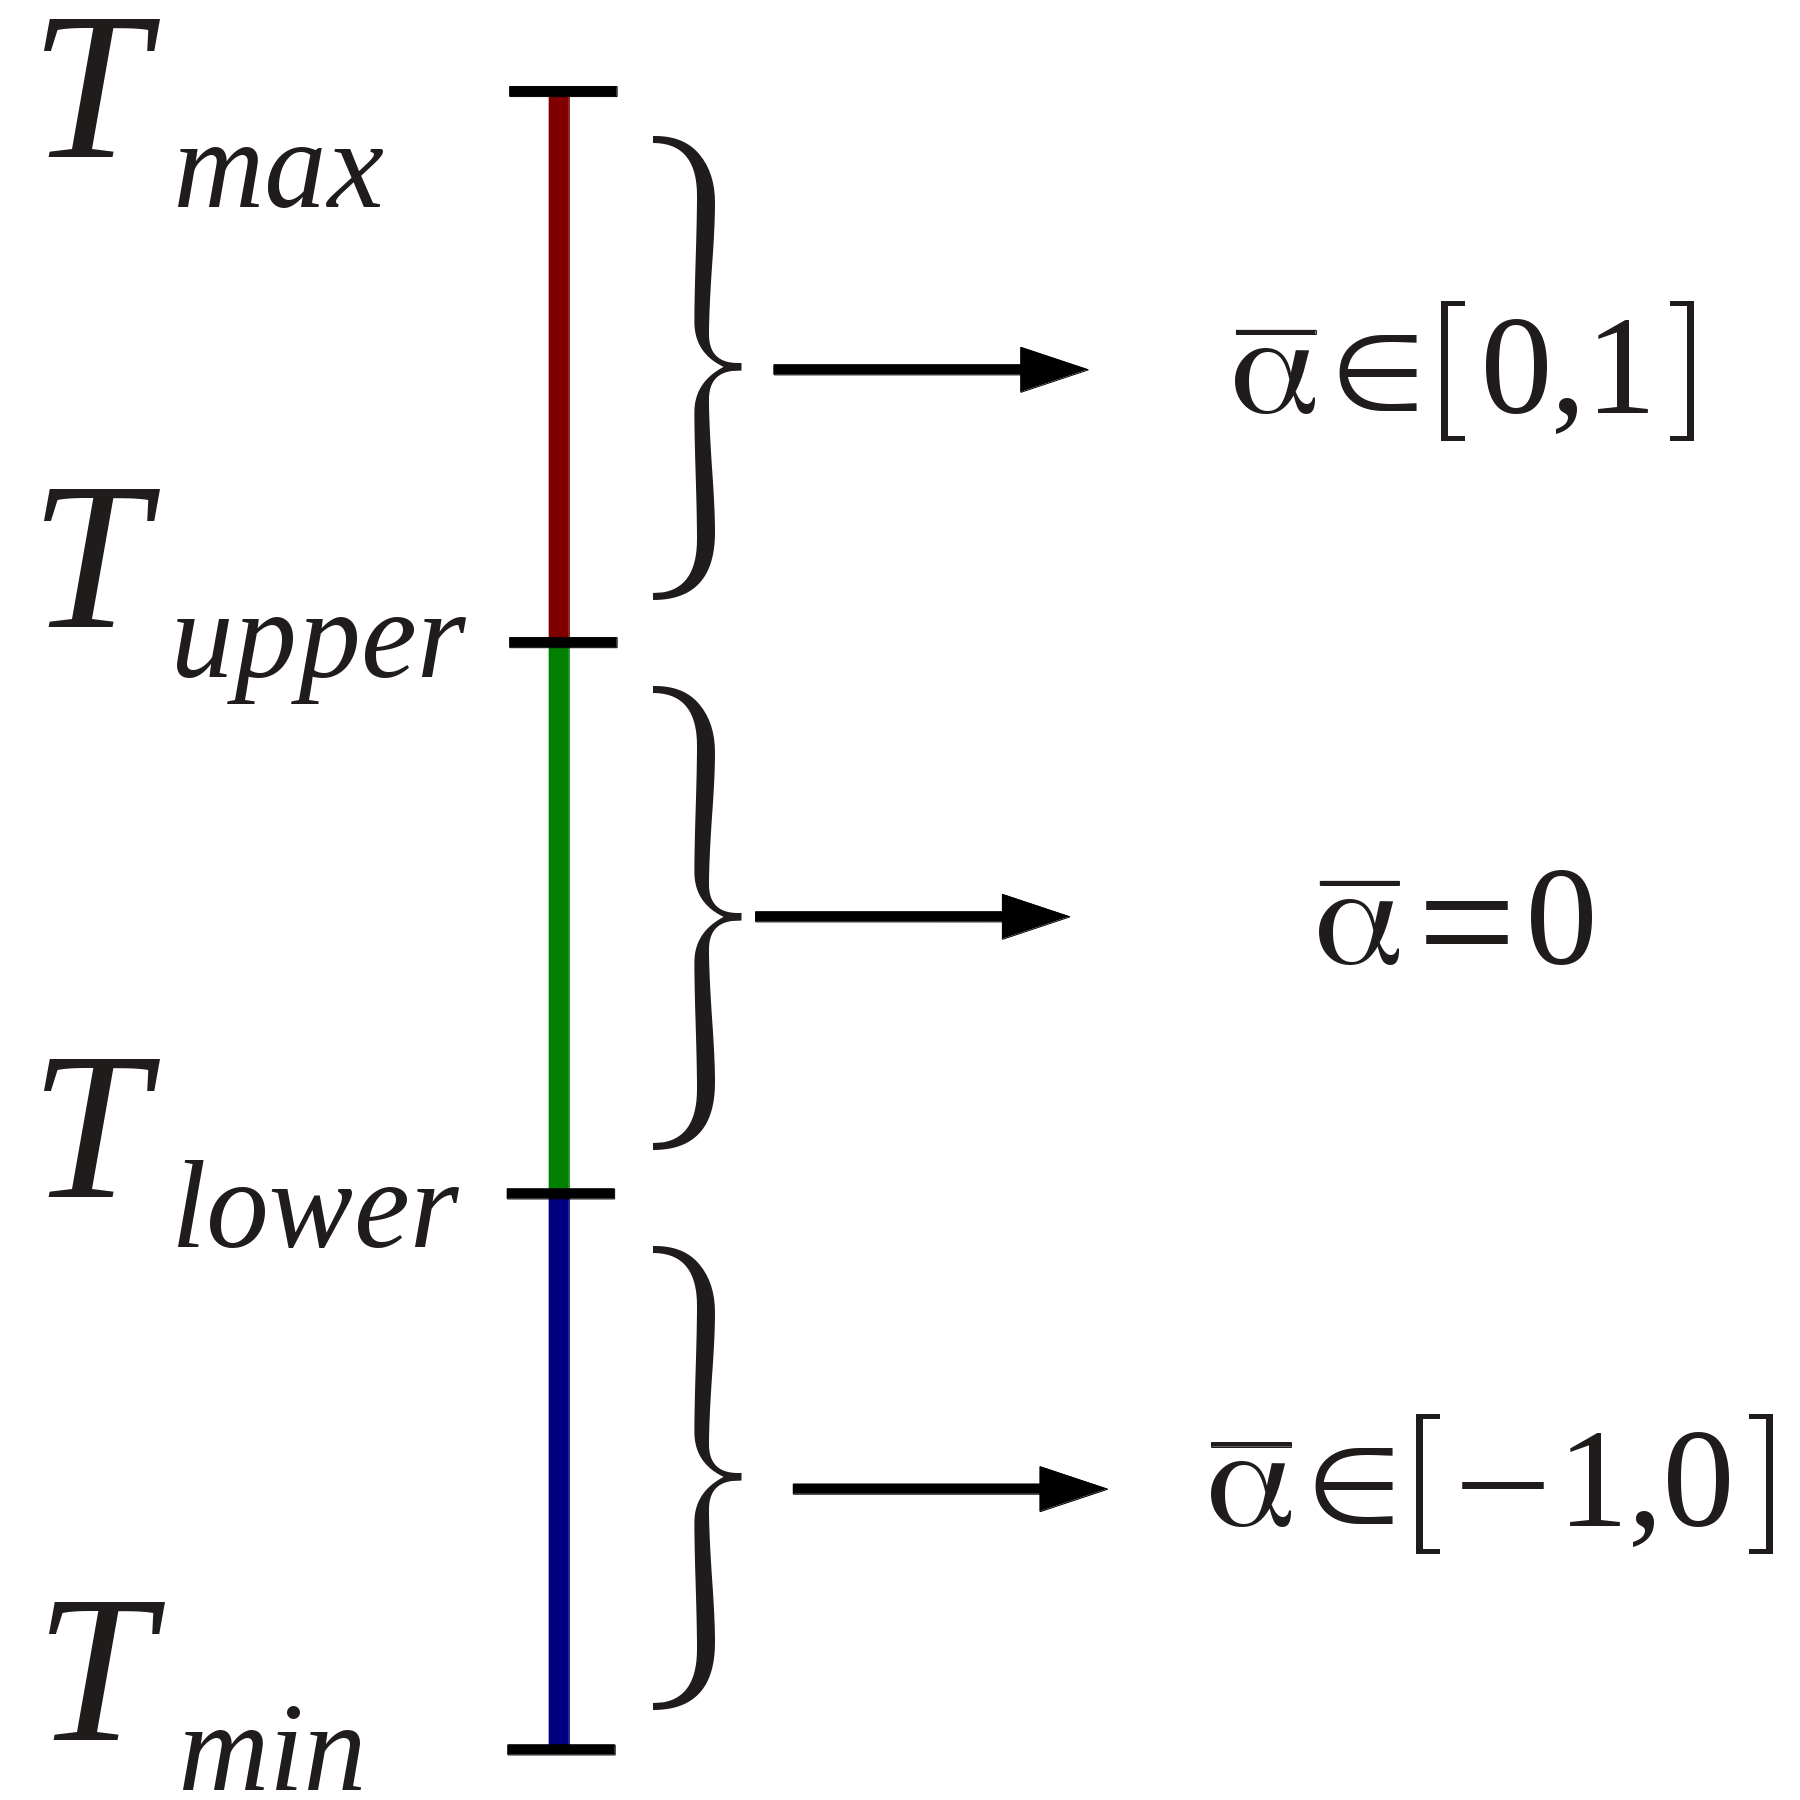
\includegraphics[scale=0.16]{TOPscale.png}
  %\caption{Computation of $\overline{\alpha}$.} 
%  \label{TopoScale}
%\end{figure}
%aaa
\end{minipage}
%$ $\\
\begin{table}[h]
\centering
\begin{tabular}{|p{2.7cm}|p{1cm}|p{1.2cm}|p{0.9cm}|p{4.7cm}|} %lcrp
\hline
\cellcolor{light-gray} Parametername & \cellcolor{light-gray} Default-wert & \cellcolor{light-gray} Zuläs-sigkeit  & \cellcolor{light-gray} B135 & \cellcolor{light-gray} Beschreibung\\
\hline
topOpt                  &  0  &  \{0,1\}          &  1   & 0:Formoptimierung, 1: Topologieoptimierung.\\
\hline
startPOR                &  0  &  [0,1]            &  0.1 & Skalierung der Startporosität.\\
\hline
porosityI               &  0  &  [0,1e6]          &  0   & Porous Inertial Resistence (maximaler Wert).\\
\hline 
porosityV               &  0  &  [0,1e6]          &  150 & Porous Viscous Resistence (maximaler Wert).\\
\hline
boundPOR                &  1  &  \{0,1\}          &  1   & Verwendung der Skalierungstechnik.\\
\hline
thresholdTOPupper       &  2  &  [0,10]           &-1e-4 & Oberer Grenzwert bei Update der Porosität.\\
\hline
thresholdTOPlower       &  1  &  \{0,1,2\}        &-0.05 & Unterer Grenzwert bei Update der Porosität.\\
\hline
\end{tabular}
\caption{Topologieoptimierung.}\label{tab:parameter10a}
\end{table}
$ $\\
\newpage
\subsection{Extrahieren der topologieoptimierten Geometrie}
Die extrahierte Geometrie kann auf Basis der Porosität oder des topologischen Gradienten erfolgen (\textbf{grad\_por}).
Mit dem Parameter \textbf{extractFolder} ist die Ordnernummer anzugeben in welcher sich der gewünschte Datensatz befindet.\\
Anstelle der Originaldaten kann $\TT_\sigma$ verwendet werden:   
\begin{figure}[htbp]
  \centering
    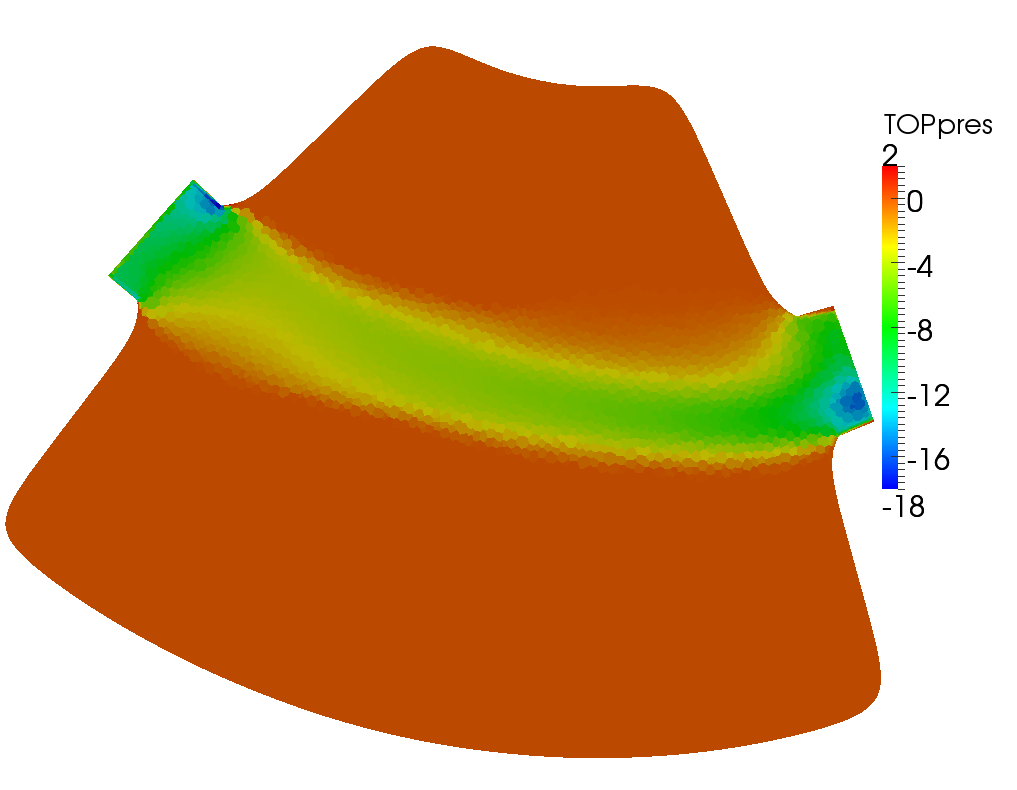
\includegraphics[scale=0.1]{TS2e5top2.png}
    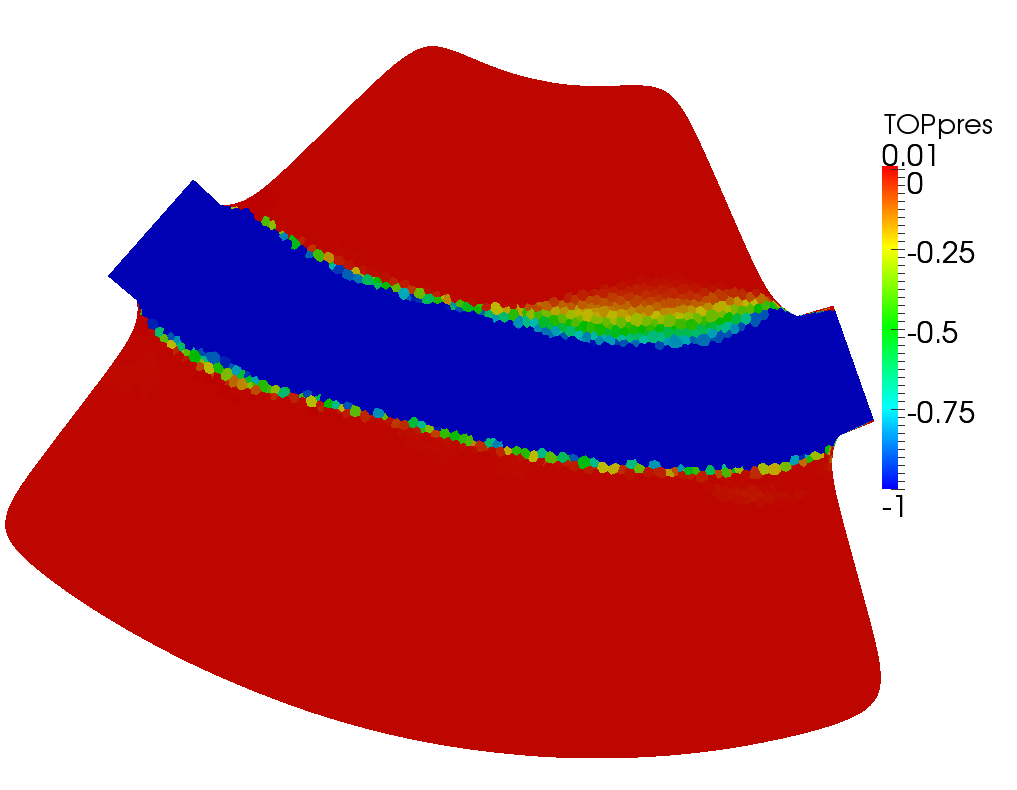
\includegraphics[scale=0.1]{TS2e5top.png}
    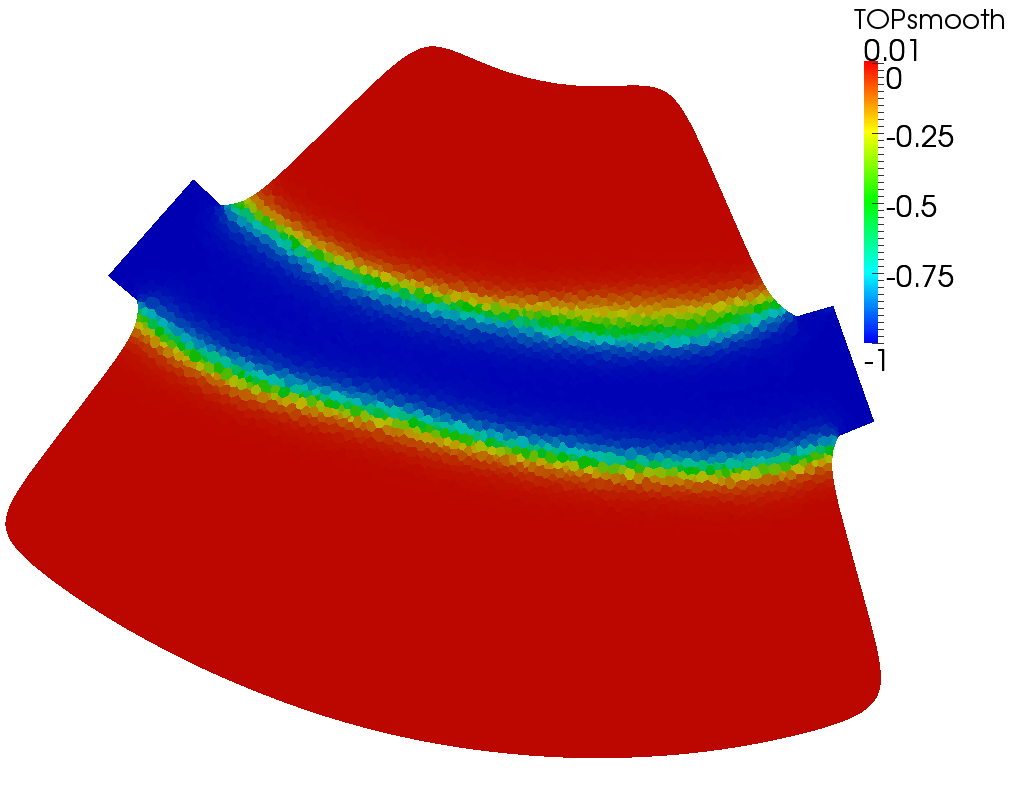
\includegraphics[scale=0.1]{TS2e5smooth.png}
  \caption{Links: $\TT\left(\bxx\right)$, \quad mitte: $\overline{\TT}\left(\bxx\right)$, \quad rechts: $\TT_\sigma\left(\bxx\right)$.} 
%\newline \textcolor{white}{.} \qquad \qquad \qquad
%Unten: Topologieopt. Geom. (2.38e-5) und formopt. Geom. (aktuell:1.59e-5).}
 \label{Topo20}
\end{figure}
%
\begin{eqnarray}
 \overline{\TT}\left(\bxx\right)=\mbox{min}\left(\mbox{max}\left(\TT\left(\bxx\right),\TT_{min}\right),\TT_{max}\right),
\end{eqnarray}
%
\begin{eqnarray}
 - \sigma \Delta \TT_\sigma + \TT_\sigma &=& \overline{\TT} \qquad \mbox{in} \; \; \Om,\\
\TT_\sigma &=& \TT_{min} \quad \mbox{auf} \; \; \Gamma_i \cup \Gamma_o,\\
\partial_n \TT_\sigma &=& 0 \qquad \, \mbox{auf} \; \; \Gamma_w \cup \Gamma_f.
\end{eqnarray}
%
Die darin enthaltenen Parameter $\TT_{min}$ und $\TT_{max}$ sind vom Benuzter durch \textbf{cutTOP} anzugeben.
Der Glättungsparameter $\sigma$ ist mit \textbf{smoothTOP} festzulegen.
%
Zur Vermeidung möglicher Überschneidungen mit den fixen Geometrien kann der Parameter \textbf{feasibleTOP} verwendet werden, um den Zulässigkeitsbereich festzulegen (siehe Abbildung \ref{extract3}).
\begin{figure}[htbp]
  \centering
    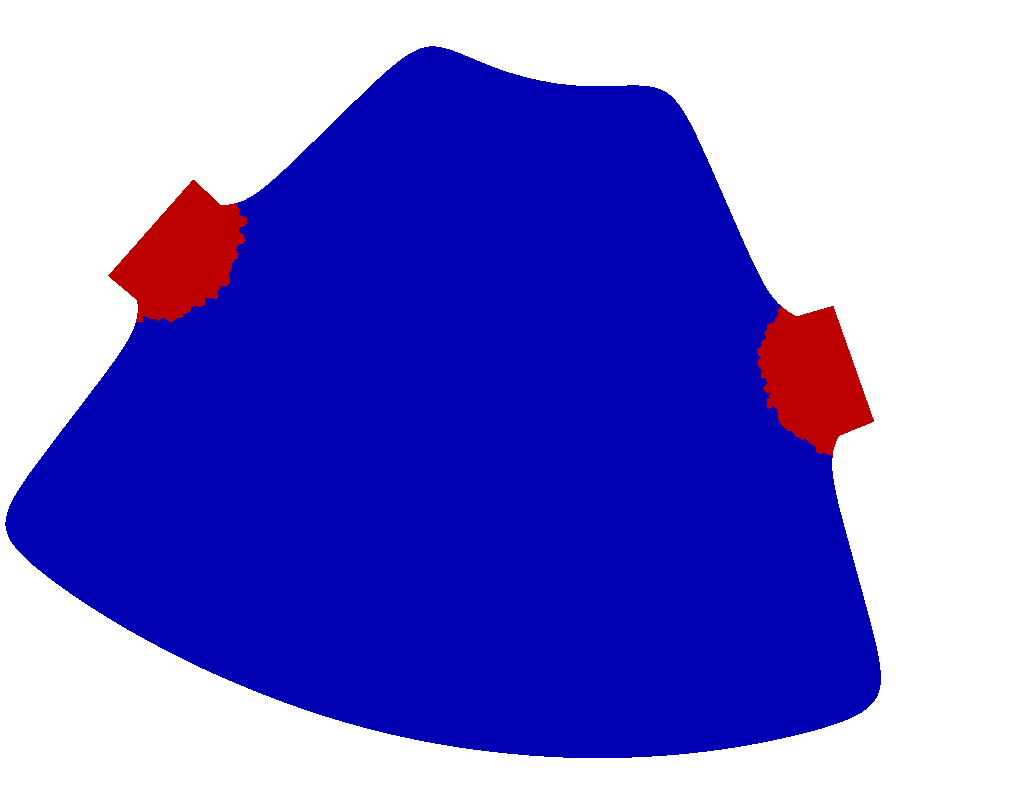
\includegraphics[scale=0.1]{TS2e5feasible.png}
    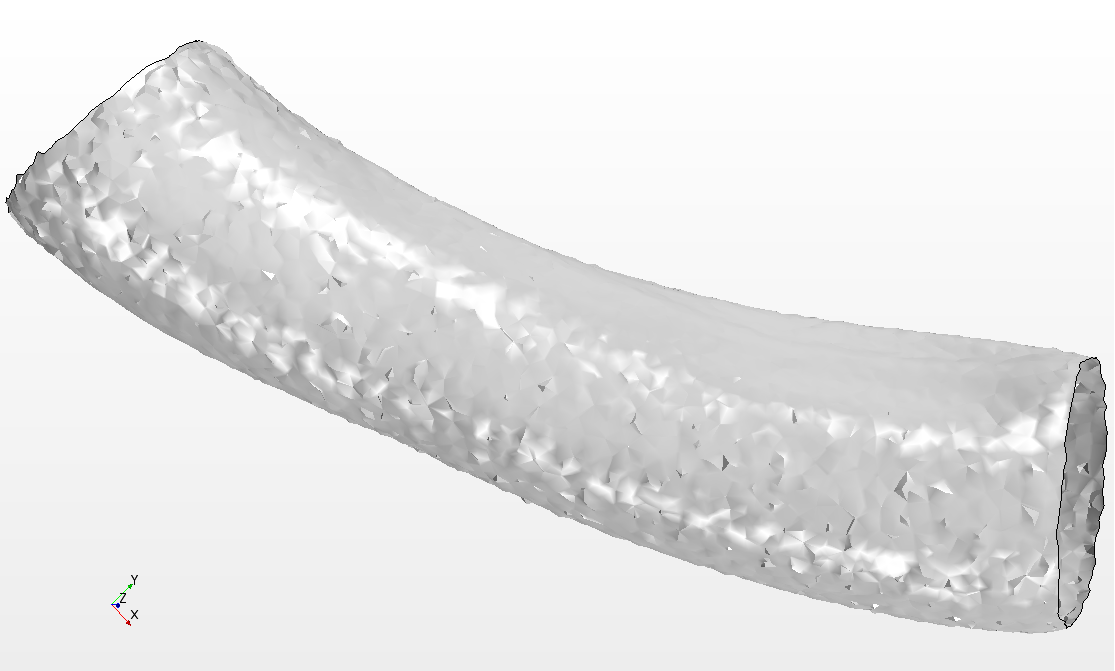
\includegraphics[scale=0.1]{TS2e5expSTL.png}
    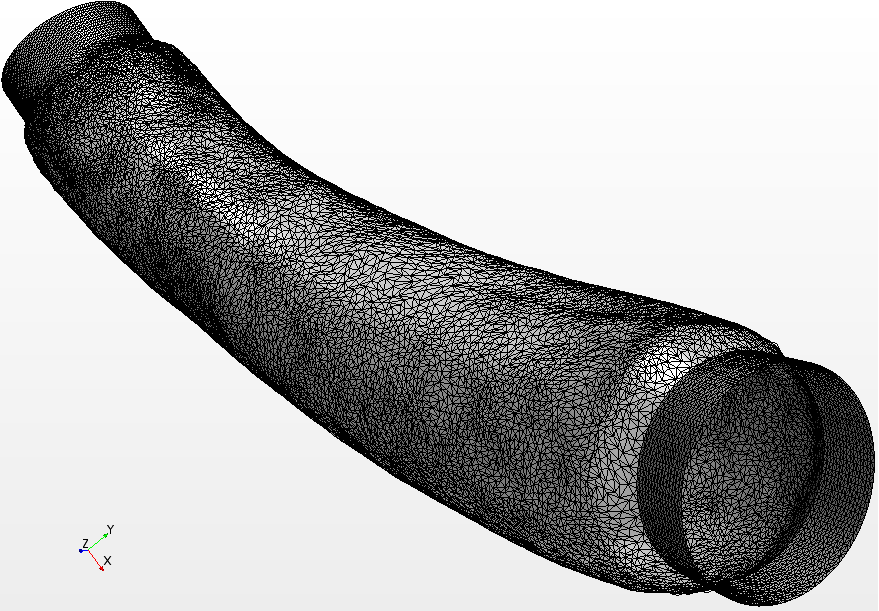
\includegraphics[scale=0.12]{TS2e5close2.png} 
\caption{Links: Unzulässigkeitsbereich (rot); Extrahierte Geometrie: mitte: \emph{wallExtract.stl}, rechts: \emph{wall.stl}}
\label{extract3}
\end{figure}
Um eine rasche Änderung der Parameter dem Benutzer zu ermöglichen erfolgt bei Aufruf der Routine \emph{topoExtractSTL} eine Auflistung der Default-Werte und eine Eingabeoption.
Die Parameter können auch in \emph{system/fvSolution/SGparameter} geändert werden.
%
\begin{table}[h]
\centering
\begin{tabular}{|p{2cm}|p{1cm}|p{1.6cm}|p{1.5cm}|p{4.4cm}|} %lcrp
\hline
\cellcolor{light-gray} Parametername & \cellcolor{light-gray} Default-wert & \cellcolor{light-gray} Zuläs-sigkeit & \cellcolor{light-gray} B135 & \cellcolor{light-gray} Beschreibung\\
\hline
grad\_por          & 0      &  \{0,1\}                & 0          & 0: verwende TOPpres; 1: verwende PORalpha.\\
\hline
extractFolder      & 1      &  \{0,1e4\}              & 60         & Geometrie extrahieren aus Ordner mit dieser Nummer.\\
\hline
cutTOP             & 2(0 0) &  \{0,1\}                & 2(-1,0.01) & Maximal- und Minimalwert.\\
\hline
smoothTOP          &   0    &  [0,1e5]                & 0.003      & Laplace Glättung der Top.Grad. Information.\\
\hline
feasibleTOP        & 2(0 0) &  [0,1e6]                & 2(0 0)     & Bereich der Unzulässigkeit am In-/Outlet in Meter.\\
\hline
thresholdTOP       &   0    &  [-1e6,1e6]             & -0.5       & Niveau-Schicht zum Erzielen der Oberfläche.\\
\hline
%
\end{tabular}
\caption{Extrahieren der topologieoptimierten Oberfläche.}\label{tab:parameter10b}
\end{table}
$ $
\newpage
\section{Initialisierung und Berechnung}
%\subsection{Ausführen der Formoptimierung}
%Nachdem ein Ordner mit der Datei \emph{parameter\_sg} und mit dem Unterordner \emph{initial\_stl} angelegt wurde, sind die Befehle:
%\begin{itemize}
%\item setupShapeGradientCCM und
%\item shapeGradientCCM
%\end{itemize}
%hintereinander auszuführen.
%$ $\\
\subsection{Ausführen der Formoptimierung}
%Die Installation kann anhand der eines Test-BSP getestet werden (Rechendauer: ca 2h):
\begin{itemize}
 \item Erstellen eines Ordneres z.B. M23Test in \$FOAM\_RUN/tutorials/incompressible/. \item Im Ordner M23Test ist die Datei parameter\_sg mit den Parametern und der Ordner initial\_stl mit den Geometriedaten anzulegen.
 \item Vom Ordner M23Test aus sind die Befehle \emph{setupShapeGradientCCM} und danach \emph{shapeGradientCCM > outtestShape.txt} auszuführen.
\end{itemize}
\subsection{Ausführen der Topologieoptimierung}
\begin{itemize}
 \item Erstellen eines Ordneres B135Test in \$FOAM\_RUN/tutorials/incompressible/. Im Ordner B135Test ist die Datei parameter\_sg mit den Parametern und der Ordner initial\_stl mit den Geometriedaten anzulegen.
 \item Vom Ordner B135Test aus sind die Befehle \emph{setupShapeGradientCCM} und \emph{topoOpt > outtestTop1.txt} auszuführen. Dies liefert TOPpres und PORalpha.
 \item Vom Ordner M23Test aus sind die Befehle \emph{topoExtractSTL} und \emph{topoOptCloseAll > outtestTop2.txt} auszuführen. Dies liefert das Zwischenergebnis wallExtract.stl und das Ergebnis
wall.stl. 
\end{itemize}
%
\subsection{Stopp und Neustart der Formoptimierung}
Zu Beginn der Formoptimierung wird automatisch die Datei \emph{STOP.txt} angelegt. Im Falle, dass die Formoptimierung beendet werden soll, so ist die Zahl in der Datei auf 0 abzuändern.
Während der Formoptimierung wird in den Iterationszahl-Ordnern, in denen eine Gitterneuvernetzung durchgeführt wurde, der Unterordner \emph{sim} angelegt.
Darin befindet sich neben der gespeicherten Simulation der vorangegangenen Iterationen auch die Datei \emph{wall.stl}.
Zusammen mit den Startgeometrien \emph{inlet.stl}, \emph{outlet.stl}, \emph{fixed.stl} und gegebenenfalls \emph{bds.stl} kann \emph{wall.stl} für eine neue Testrechnung verwendet werden.\\
Falls die Geometrieänderung bezüglich der Startgeometrie berechnet werden soll, so ist diese in der Datei \emph{wall0.stl} im Ordner \emph{initial\_stl} zu speichern und der Parameter \textbf{restart\_opt} auf 1 zu setzen (siehe Tabelle \ref{tab:parameter9}). 
Wenn die selbe Skalierung der Zielfunktionale gewünscht ist, so ist der Parameter \textbf{damp} im \emph{parameter\_sg} File anzugeben.
Diese Werte werden stets in der \emph{Testlauf\_Info.txt} Datei gespeichert.
%
\section{Datenauswertung und Visualisierung}
\subsection{Ausgabedaten}
Während der Form- und Topologieoptimierung werden in jeder Iteration die relevanten Daten 
(siehe Tabelle \ref{tab:output1} und \ref{tab:output2}) in den entsprechenden Ordnern (Bezeichnung gemäß der Iterationszahl) gespeichert.
Die aktuellen Geometriedaten werden in \textbf{polyMesh} gespeichert. 
Weitere Daten wie Zielfunktionswerte, verwendete Schrittweiten etc. befinden sich im Textfile \textbf{Testlauf\_Info.txt}.
\begin{table}[h]
\centering
\begin{tabular}{|p{1.8cm}|p{1.4cm}|p{1.9cm}|p{6cm}|} %lcrp
\hline
\cellcolor{light-gray} Ausgabedatei & \cellcolor{light-gray} Dimension & \centering \cellcolor{light-gray} Auftreten &  \cellcolor{light-gray}  Beschreibung  \\
\hline
\centering U0          & \centering Vektor     & \centering Gebiet, Rand &      Lösung $\buu$ der primalen Gleichung (Geschwindigkeit).\\
\hline
\centering p0          & \centering Skalar     & \centering Gebiet, Rand &      Lösung $ p$ der primalen Gleichung (Druck).\\
\hline
\centering density0    & \centering Skalar     & \centering Gebiet, Rand &      Verwendete Dichte in der Navier - Stokes Gleichung.\\
\hline
\centering Vunif       & \centering Vektor     & \centering Gebiet, Rand &      Lösung $\bvv$ der adjungierten Gleichung (adjungierte Geschwindigkeit) hinsichtlich Erzielens einer gleichmäßigen Ausströmung.\\
\hline
\centering Vpres       & \centering Vektor     & \centering Gebiet, Rand &      Lösung $\bvv$ der adjungierten Gleichung (adjungierte Geschwindigkeit) hinsichtlich Minimierung des Totaldruckverlustes.\\
\hline
\centering Sg0u        & \centering Skalar     & \centering Rand   &      Negativer Formgradient (skaliert).\\ 
\hline
\centering Sg00u       & \centering Skalar     & \centering Rand   &      Negativer Formgradient (skaliert): Anteil von $\JJ_1$, $\JJ_2$.\\ 
\hline
\centering Sg0Lu       & \centering Skalar     & \centering Rand   &      Negativer Formgradient (skaliert): Anteil geometrische Restriktion.\\ 
\hline
\centering SgVpres0    & \centering Skalar     & \centering Rand   &      Negativer Formgradient (skaliert): Anteil von $\JJ_2$ (Totaldruckverlust).\\ 
\hline
\centering SgVunif0    & \centering Skalar     & \centering Rand   &      Negativer Formgradient (skaliert): Anteil von $\JJ_1$ (gleichmäßige Ausströmung).\\ 
\hline
\centering GeomChange  & \centering Skalar     & \centering Rand   &      Geometrieänderung zur Ausgangsgeometrie (in Meter).\\     
\hline
\centering Distance    & \centering Skalar     & \centering Rand   &      Distanz zur Bauraumgeometrie (in Meter).\\
\hline
\centering Sg0Pu       & \centering Skalar     & \centering Rand, Point &      Negativer Formgradient - Laplace-Beltrami (skaliert).\\ 
\hline
\end{tabular}
\caption{Ausgabedaten Formoptimierung.}\label{tab:output1}
\end{table}
%
\begin{table}[h]
\centering
\begin{tabular}{|p{1.8cm}|p{1.4cm}|p{1.5cm}|p{6.2cm}|} %lcrp
\hline
\cellcolor{light-gray} Ausgabedatei & \cellcolor{light-gray} Dimension & \centering \cellcolor{light-gray} Auftreten &  \cellcolor{light-gray}  Beschreibung  \\
\hline
\centering TOPpres     & \centering Skalar     & \centering Gebiet &      Topologische Sensitivität Totaldruckverlust.\\
\hline
\centering TOPmix      & \centering Skalar     & \centering Gebiet &      Effektive Topologische Sensitivität.\\
\hline
\centering PORalpha    & \centering Skalar     & \centering Gebiet &      Porosität.\\
\hline
\centering 1/TOPsmooth & \centering Skalar     & \centering Gebiet &      Geglättete Daten $\TT_\sigma$ (\textbf{smoothTOP}).\\
\hline
\centering 1/TOPfea    & \centering Skalar     & \centering Gebiet &      Zulässigkeitsbereich (\textbf{feasibleTOP}).\\
\hline
\end{tabular}
\caption{Ausgabedaten Topologieoptimierung.}\label{tab:output2}
\end{table}
%
$ $\\
%\newpage
\subsection{Visualisierung mit ParaView}
Zur Visualisierung der Daten empfiehlt sich die Verwendung von ParaView.
Nach Installation im Zuge der OpenFOAM Setzung kann paraView mit dem Befehl \emph{paraFOAM} im Ordner, mit den zu visualisierenden Daten, aufgerufen werden.
Folgende Darstellungsmöglichkeiten der Daten können in paraView verwendet werden (siehe Abbildung \ref{fig:paraview} - \ref{fig:paraviewTopo}): 
\begin{itemize}
\item \emph{Point Field} und \emph{Volume Field} Information auf der Oberfläche (Sg0P, GeomChange),
\item Vektorfeld mit \emph{Glyph} (U0),
\item Querschnitt mit \emph{Clip} bzw. \emph{Slice} oder Kontur mit \emph{Contour} (TOPpres, PORalpha, TOPsmooth),
\item STL-Daten mit \emph{File>Open} (wallExtract.stl).
\end{itemize}
%
%
%
\begin{figure}[h]
    \centering
    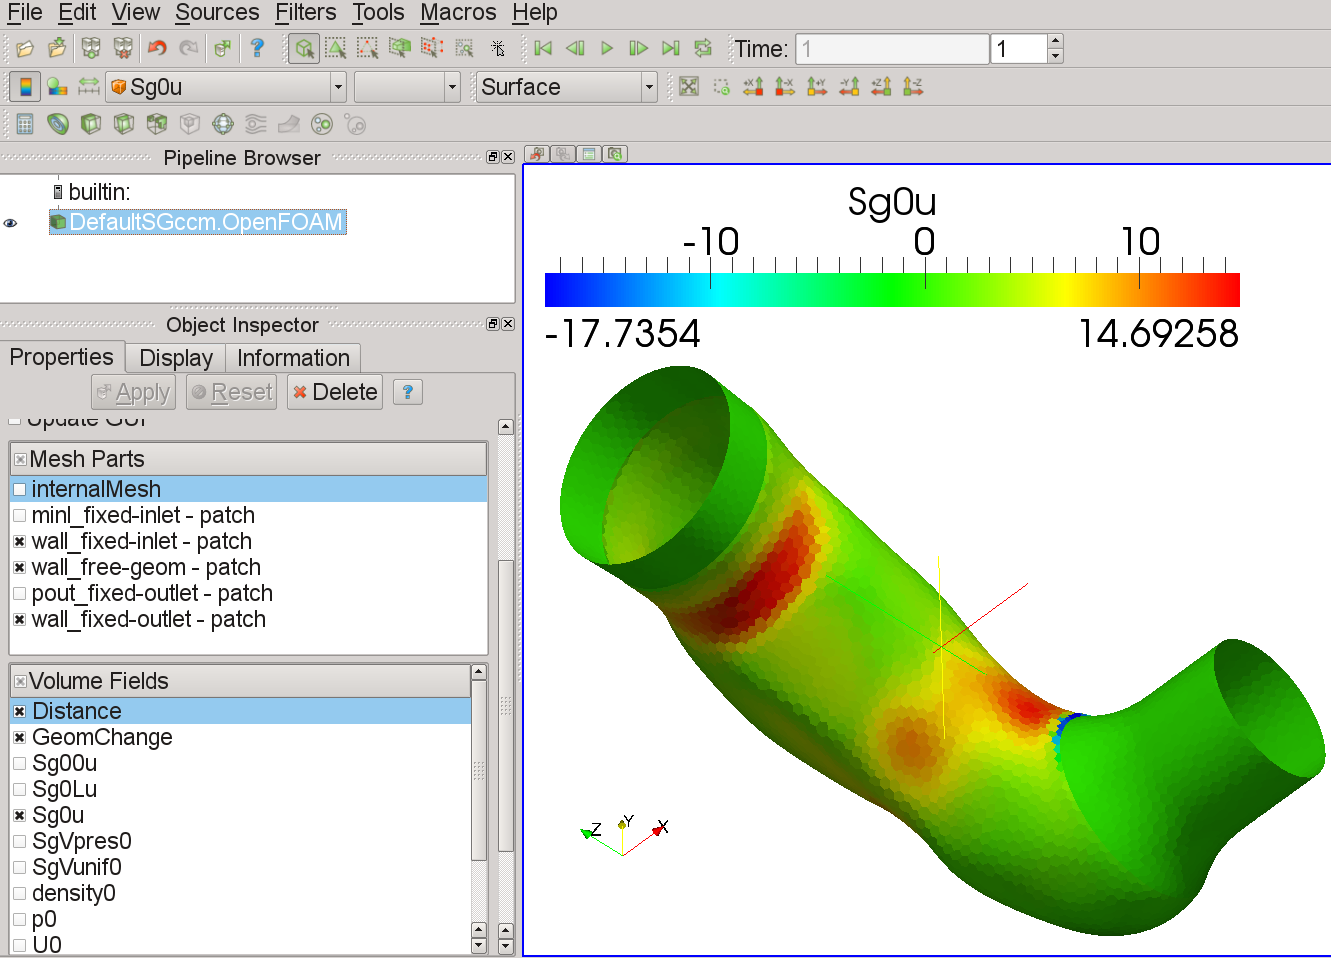
\includegraphics[scale=0.23]{paraview1.png}
   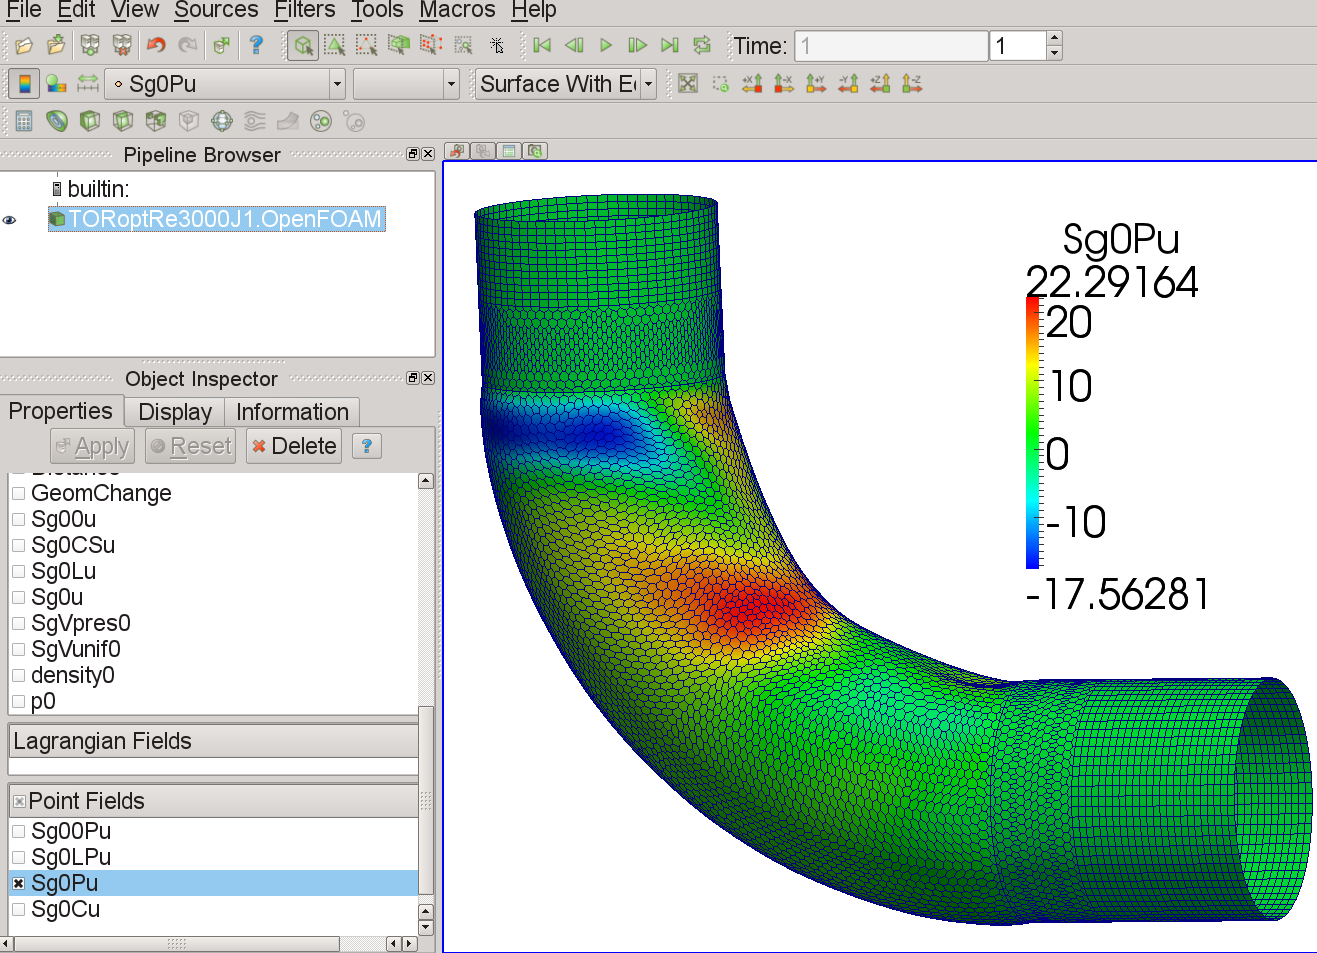
\includegraphics[scale=0.23]{paraview3.png}
  \caption{Verwendung von ParaView: VolumeFields, PointFields.} 
\label{fig:paraview}
\end{figure}
%
%
%\newpage
%
%\begin{figure}[h]
%    \centering
%    \includegraphics[scale=0.26]{distance_ds_invalid.png}
%%    \includegraphics[scale=0.26]{distance_ds_invalid2.png}
%  \caption{Bauraumverletzung: Darstellung von Distance in ParaView.} 
%\label{fig:paraviewBauraum}
%\end{figure}
%%
\begin{figure}[htbp]
  \centering
   \includegraphics[scale=0.11]{S200por8.png}
   \includegraphics[scale=0.11]{S200top7.png}
   \includegraphics[scale=0.11]{S200con7.png}
  \caption{Porosität, Effektiver Top.-Grad und Kontur.} 
  \label{fig:paraviewTopo}
\end{figure}
%
\begin{landscape}
\includegraphics[scale=0.5]{testlauf_info161.png}\\
$ $\\ 
\includegraphics[scale=0.5]{testlauf_info162.png}\\
$ $\\ 
\includegraphics[scale=0.5]{testlauf_info163.png}
\end{landscape}
%
%\begin{figure}[h]
%    \centering
%    \includegraphics[scale=0.45]{testlauf_info3.png}\\
%$ $\\ 
%    \includegraphics[scale=0.45]{testlauf_info4.png}
%  \caption{Testlauf\_Info - Datei.}
%\label{fig:testlauf}
%\end{figure}
%
%
%
%Hinweise zu den Neuerungen kurz im Überblick:
%- \textbf{iterPri} ist groß zu wählen: Die primale Lösung ist auskonvergiert wenn die gewünschte Genauigkeit (\textbf{stop\_accuracyPri}) erreicht ist.
%Wenn die maximale Iterationszahl erreicht ist ohne gewünschter Genauigkeit so wird die Lösung als nicht auskonvergiert angesehen und es erfolgt in der Liniensuche eine Verkleinerung der Schrittweite.
%- wird in STOP.txt der Wert auf 0 gesetzt wird die Formoptimierung 'kontrolliert' beendet.
%- Übergangsrestriktion Methode 1+4 hat sich bei meinen Tests als gut erwiesen: 
%uer\_linear            10; 
%uer\_fix\_faces         1;
%scaleLB               1e-5;
%scaleShapeGradientFix 0;
%- turb\_model: Achtung hier hat sich die Reihenfolge geändert: 0=DNS, 1=RealizableKepsilon, 2=StdKepsilon, 3=RSM 
\subsection{Struktogramm}
Ein Struktogramm zur Software befindet sich in Abbildung \ref{fig:struktogramm}.
Berechnungsschritte sind in eckigen Feldern und Abfragen in abgerundeten Feldern dargestellt.
Die wesentlichen Softwareteile sind bei den jeweiligen Berechnungsschritten in grauer Schrift angegeben.
In der Ausgabedatei \emph{Testlauf\_Info.txt} befindet sich am Ende der Zeile jeder Iteration in eckigen Klammern ein Zahlencode.
Dieser Zahlencode gibt den Verlauf der Schrittweitensteuerung innerhalb der jeweiligen Iteration an.\\
Die Ziffern finden sich im Struktogramm in Abbildung \ref{fig:struktogramm} wieder, deren Bedeutung ist in Tabelle \ref{tab:zahlencode} angegeben.
$ $\\ 
\begin{table}[h]
\begin{tabular}{|p{0.8cm}|p{10cm}|} %lcrp
\hline
\cellcolor{light-gray} Ziffer & \cellcolor{light-gray} Bedeutung \\
\hline
0             & Schritt akzeptiert / Ende der Iteration.\\
\hline
1             & Gitterneuvernetzung.\\
\hline
2             & Gitterqualitätskriterien nicht erfüllt für gesamte Geometrie .\\
\hline 
3             & Bauraumüberschreitung bei Verwendung von Barriere-Methode.\\
\hline
33            & Bauraumüberschreitung der Startgeometrie bei Verwendung von Barriere-Methode.\\
\hline
4             & Zielfunktional fällt nicht gemäß Armijo - Regel.\\
\hline
6             & Primaler Löser konvergiert nicht.\\
\hline
66            & Primaler Löser konvergiert nicht bei der Startkonfiguration.\\
\hline
7             & Gitterqualitätskriterien nicht erfüllt für Geometrie \emph{wall}.\\
\hline
8             & Oberflächenqualität unzureichend.\\
\hline
9             & Vom Benutzer erzwungene Neuvernetzung.\\
\hline
\end{tabular}
\caption{Zahlencode Liniensuche Formoptimierung.}\label{tab:zahlencode}
\end{table}
%
%
%
%    
\begin{figure}[htbp]
    \centering
    \includegraphics[scale=0.47]{struktogramm16.png}
  \caption{Struktogramm Formoptimierung.} 
\label{fig:struktogramm}
\end{figure}
%
$ $\\
$ $\\
%
\end{document}







